\documentclass[12pt]{report}
\usepackage{multirow}
\usepackage{rotating}
\usepackage{hhline}
\usepackage[]{graphicx}
\usepackage[left=1.25in, right=1in,top=1in,bottom=1in,headheight=6pt, a4paper]{geometry}
\usepackage{titling}
\usepackage{booktabs}
\usepackage{natbib}
\usepackage{url}
% \usepackage{biblatex}
% \usepackage{times}
\usepackage{microtype}
\usepackage[utf8x]{inputenc}
\usepackage{xcolor}
\usepackage{datetime2}
\usepackage{array}
\usepackage{enumitem}
\usepackage[font=normalsize,tableposition=top]{caption}
\usepackage{etoolbox}\usepackage{setspace}
\usepackage[explicit]{}
\usepackage{algpseudocode, algorithm}
\usepackage{amsmath}
\usepackage{amsfonts}
\usepackage{amssymb}
\usepackage{hyperref}
\usepackage{pgfgantt}
\usepackage{adjustbox}
\usepackage{multicol}
\usepackage{mathptmx}
\usepackage{titlesec}
\usepackage{setspace}
\usepackage{import}
\usepackage{enumitem}
\usepackage{bm}
\usepackage{amsmath, amsfonts}
\usepackage{pdflscape}
\usepackage{everypage-1x}
\usepackage{wrapfig}
\usepackage{scrextend}
\usepackage{etoolbox}
\usepackage{appendix}
\usepackage{ragged2e}
\usepackage{tabularx}
\usepackage{longtable}

\renewcommand\appendixtocname{APPENDIX}
\renewcommand\appendixpagename{APPENDIX}
\renewcommand{\bibname}{REFERENCES}

%\usetikzlibrary{positioning}
% \ganttset{group/.append style={orange},
% milestone/.append style={red},
% progress label node anchor/.append style={text=red}}

\linespread{1.3}
\setlength{\parskip}{6pt}
\setlength{\parindent}{0em}


%--------------------



% Column for Letter of Aproval
\newcolumntype{Y}{>{\raggedright\arraybackslash}X}

%------ SET DOCUMENT GEOMETRY ------%
\usepackage{geometry}
\geometry{a4paper, left=1.25in, top=1in, bottom=1in, right=1in}


%------ FORMAT CHAPTER, SECTION, AND SUBSECTION TITLE ------%
  \titleformat{\chapter}{
  \normalfont\fontsize{12}{15}\bfseries
  }{\thechapter}{1em}{}

  \titleformat{\section}{
  \normalfont\fontsize{12}{15}\bfseries
  }{\thesection}{1em}{}

  \titleformat{\subsection}{
  \normalfont\fontsize{12}{15}\bfseries
  }{\thesubsection}{1em}{}

  \titlespacing{\chapter}{0pt}{-0.5in}{-0.5em}
  \titlespacing{\section}{0pt}{0pt}{-1em}
  \titlespacing{\subsection}{0pt}{0pt}{-1em}

  % Sub Section
  \setcounter{secnumdepth}{3}
  \titlespacing{\subsection}{0pt}{*1.5}{*0.5}

%------ SET SPACING AND INDENTS ------%
\renewcommand{\baselinestretch}{1.5} 
\setlength{\parindent}{0pt}
\setlength{\parskip}{12pt}


%------ SETUP LINKS ------%
\usepackage{hyperref}
\hypersetup{
    colorlinks,
    citecolor=black,
    filecolor=black,
    linkcolor=black,
    urlcolor=black
}


%------ FORMAT TABLE OF CONTENTS ------%
\usepackage{tocloft}


\cftsetindents{section}{1.4em}{1.75em}
\cftsetindents{subsection}{3.2em}{2.6em}
\setlength{\cftbeforetoctitleskip}{-2.5em}
\setlength{\cftbeforechapskip}{0.25em}

\renewcommand{\cftchapleader}{\dotfill}

\renewcommand{\cftdotsep}{1.5}
\renewcommand{\cftsecfont}{\normalfont}
\renewcommand{\cftsecpagefont}{\normalfont}

\setlength{\cftbeforeloftitleskip}{-2.5em}
\setlength{\cftbeforelottitleskip}{-2.5em}

\setlength{\cftfigindent}{0pt}
\setlength{\cfttabindent}{0pt}

\renewcommand{\cftfigfont}{Figure }
\renewcommand{\cfttabfont}{Table }


%------ FORMAT TABLE CAPTIONS ------%
\usepackage{caption} 
\captionsetup[table]{skip=10pt}



\newcommand{\Lpagenumber}{\ifdim\textwidth=\linewidth\else\bgroup
  \dimendef\margin=0 %use \margin instead of \dimen0
  \ifodd\value{page}\margin=\oddsidemargin
  \else\margin=\evensidemargin
  \fi
  \raisebox{\dimexpr -\topmargin-\headheight-\headsep-0.5\linewidth}[0pt][0pt]{%
    \rlap{\hspace{\dimexpr \margin+\textheight+\footskip}%
    \llap{\rotatebox{90}{\thepage}}}}%
\egroup\fi}
\AddEverypageHook{\Lpagenumber}%


\newcommand{\theinstitute}{Faculty of Humanities and Social Sciences }
\newcommand{\thecampus}{Lalitpur Engineering College }
\newcommand{\thedepartment}{Department of Computer Application }
\newcommand{\thedepartmentAddress}{Lalitpur, Nepal }
\newcommand{\thedepartmentFullAddress}{Patan, Lalitpur, Nepal }
\newcommand{\theprogramcoordinator}{Er. Bibat Thokar }
\newcommand{\theHOD}{Er. Bibat Thokar }
\newcommand{\authorWithAnd}{ Sushant Bramhacharya (LEC077BCA08) }


\title{LabXplorerX: Interactive Learning Environment}
\author{ Sushant Bramhacharya (LEC077BCA08) }
\newcommand{\theroll}{
  % LEC077BCA01\\LEC077BCA08
}
\date{September, 2024}
\newcommand{\thesupervisor}{Er. Bibat Thokar}



\begin{document}

\pagenumbering{roman}

\thispagestyle{empty}
\begin{center}
\begin{spacing}{1.6}


\includegraphics[scale=0.75]{img/Graphics/LEC.jpeg}

\textbf{
\large{TRIBHUVAN UNIVERSITY}\\
\MakeUppercase{\large{\theinstitute}}\\
\MakeUppercase{\large{\thecampus}}}

\vspace{0.5cm}

\hspace{-8cm}
% \textbf{PROJECT NO.: \theroll}

\vspace{0.5cm}

\textbf{\MakeUppercase{\thetitle}\\
\vspace{0.5cm} 
BY \\ 
\MakeUppercase{\theauthor}}

\vspace{0.5cm}

\textbf{A PROJECT PROPOSAL\\
SUBMITTED TO THE \MakeUppercase{\thedepartment}\\ IN PARTIAL FULFILLMENT OF THE REQUIREMENT FOR\\ THE DEGREE OF BACHELORS IN COMPUTER APPLICATION}
\bigskip

\par
\textbf{\MakeUppercase{\thedepartment}}\\
\textbf{\MakeUppercase{\thedepartmentAddress}}
\vspace{1cm}

\textbf{\MakeUppercase{\thedate}}


\end{spacing}
\end{center}

\clearpage
\begin{center}
\begin{spacing}{1.6}
\thispagestyle{empty}


\includegraphics[scale=0.75]{img/Graphics/LEC.jpeg}

\textbf{
\large{Tribhuvan University}\\
\large{\theinstitute}}\\
\vspace{0.5cm}
\textbf{\MakeUppercase{\thetitle}\\
\vspace{0.5cm} 
Submitted to\\ 
\thedepartment\\
\thecampus}\\
\vspace{0.5cm}

\textbf{In partial fulfillment of the requirement for the degree of Bachelors in Computer Application}
\bigskip

\par

\textbf{
Submitted by\\
\theauthor\\
\MakeUppercase{\thedate}}\\
\vspace{1cm}
\textbf{
Under the Coordination of\\
\thesupervisor
}
\end{spacing}
\end{center}

\clearpage
% \chapter*{\centerline{COPYRIGHT \textcopyright}}
\addcontentsline{toc}{chapter}{COPYRIGHT}
\vspace{-0.5cm}

The author has agreed that the library, \thedepartment, \theinstitute, \thecampus, may make this project
work freely available for inspection. Moreover the author has agreed that the
permission for extensive copying of this project work for scholarly purpose may be
granted by the professor(s), who supervised the project work recorded herein or, in
their absence, by the Head of the Department, wherein this project work was done. It
is understood that the recognition will be given to the author of this project work and
to the \thedepartment, \theinstitute, \thecampus \ in any use of the material of this project work. Copying of publication or other use of
this project work for financial gain without approval of the \thedepartment, \theinstitute, \thecampus \ and author’s
written permission is prohibited.

Request for permission to copy or to make any use of the material in this thesis in
whole or part should be addressed to:

\vspace{1cm}

Head\\
\thedepartment\\
\theinstitute, \thecampus\\
\thedepartmentFullAddress

\chapter*{\centerline{DECLARATION}}
\addcontentsline{toc}{chapter}{DECLARATION}
\vspace{-0.5cm}
I declare that the work hereby submitted for Bachelors in Computer Application at the \thedepartment, \thecampus \ entitled "\textbf{\thetitle}" is my own work and has not been previously submitted by
me at any university for any academic award.
I authorize the \thedepartment, \thecampus \ to lend this project work
to other institutions or individuals for the purpose of scholarly research.

\vspace{1cm}

\textbf{\theauthor} \\
\theroll \\
\thedate


\addcontentsline{toc}{chapter}{SUPERVISOR'S  RECOMMENDATION}
\begin{figure}
    \centering
    
\includegraphics[width=1.2in]{img/Graphics/TUlogo.png}
\end{figure}
\begin{center}
    {\fontsize{14pt}{18}\selectfont
    \textbf{Tribhuvan University\\
    Faculty of Humanities and Social Sciences\\
    Lalitpur Engineering College\\
    \vspace{0.2in}
    Supervisor's Recommendation\\}}
\end{center}

\vspace{-0.5cm}
The undersigned certify that he have read and recommend to the \thedepartment \ for acceptance, a project work entitled “\textbf{\thetitle}”, submitted by \textbf{\authorWithAnd} in partial fulfillment of the requirement
for the award of the degree of “\textbf{Bachelors in Computer Application}”.

\vspace{1cm}
\rule{0.5\textwidth}{0.4pt}\\
\textbf{Project Supervisor}\\
\thesupervisor\\
BCA Coordinator, Lecturer\\
\thedepartment, Lalitpur Engineering College\\

\vspace{1cm}
\thedate
\restoregeometry
\addcontentsline{toc}{chapter}{LETTER OF APPROVAL}
\begin{figure}
    \centering
    
\includegraphics[width=1.2in]{img/Graphics/TUlogo.png}
\end{figure}
\begin{center}
    {\fontsize{14pt}{18}\selectfont
    \textbf{Tribhuvan University\\
    Faculty of Humanities and Social Sciences\\
    Lalitpur Engineering College\\
    \vspace{0.2in}
    LETTER OF APPROVAL\\}
    }
\end{center}
This is to certify that this project prepared by Sushant Bramhacharya entitled “\textbf{\thetitle}” in partial fulfillment of the requirements for the degree of Bachelor in Computer Application has been evaluated. In our opinion it is satisfactory in the
scope and quality as a project for the required degree.\\
\begin{center}
    {\fontsize{14pt}{18}\selectfont
    \begin{table}[ht]
        \begin{tabularx}{\textwidth}{|Y|Y|}
        \hline
        &\\
        &\\
        &\\
        ..................................................................&..................................................................\\
        &\\
        Er. Bibat Thokar & Er. Bibat Thokar \\
        Project Supervisor & BCA Program Coordinator \\
        Department of Computer Application & Department of Computer Application\\
        Lalitpur Engineering College & Lalitpur Engineering College \\
        &\\
        \hline
        &\\
        &\\
        &\\
        ..................................................................&..................................................................\\
        &\\
        Internal Examiner&External Examiner  \\
        &\\
        &\\
        \hline
        \end{tabularx}
        \end{table}
    }
\end{center}
\newgeometry{left=1.5in, top=2.5in, bottom=1in, right=1in}
\chapter*{\centerline{DEPARTMENTAL ACCEPTANCE}}
\addcontentsline{toc}{chapter}{DEPARTMENTAL ACCEPTANCE}
\vspace{-0.5cm}
The project work entitled “\textbf{\thetitle}”, submitted by \textbf {\authorWithAnd }in
partial fulfillment of the requirement for the award of the degree of “\textbf{Bachelors of Computer Application}” has been accepted as
a genuine record of work independently carried out by the student in the department.

\vspace{5cm}

\begin{addmargin}[5.5cm]{0em}
\rule{0.62\textwidth}{0.4pt}\\
\textbf{\theHOD}\\
BCA Coordinator\\
\thedepartment,\\
\thecampus,\\
\theinstitute,\\
Tribhuvan University,
Nepal.\\
\end{addmargin}

\vspace{2cm}

\thedate

\restoregeometry
\chapter*{\centerline{ACKNOWLEDGMENT}}
\addcontentsline{toc}{chapter}{ACKNOWLEDGMENT}
\vspace{-0.5cm}
This project work would not have been possible without the guidance and the help of
several individuals who in one way or another contributed and extended their
valuable assistance in the preparation and completion of this study.


First of all, I would like to express my sincere gratitude to my supervisor, \textbf{\thesupervisor}, of \textbf{\thecampus} for providing invaluable guidance, insightful comments, meticulous suggestions, and encouragement throughout the duration of
this project work. My sincere thanks also goes to the BCA coordinator, \textbf{\theprogramcoordinator}, for coordinating the project works, providing astute criticism, and having
inexhaustible patience.

Furthermore, we would like to extend our gratitude to the entire faculty of the \thedepartment. Their dedication to fostering creativity, critical thinking, and technical proficiency has been useful in our project's development. The support and guidance received from our teachers have empowered us to transform our vision into a reality.

I am also grateful to my classmates and friends for offering me advice and moral
support. To my family, thank you for encouraging me in all of my pursuits and
inspiring me to follow my dreams. I am especially grateful to my parents, who
supported me emotionally, believed in me and wanted the best for me.

\vspace{1cm}

\textbf{\theauthor} \\
\theroll \\
\thedate

%==============================Abstract Page=================================================
\chapter*{\centerline{ABSTRACT}}
\addcontentsline{toc}{chapter}{ABSTRACT}
\thispagestyle{plain} 
% Abstract (200 to 250 Words)
\vspace{-0.5cm}

LabXplorer is an innovative web application developed using the PERN (PostgreSQL, Express.js, React, Node.js) stack and Phaser.js, designed to revolutionize science education by providing interactive virtual experiments. This platform offers a user-friendly interface where students can conduct various experiments, track their progress, and showcase their scientific achievements. By leveraging real-time, visually engaging simulations, LabXplorer enhances students' understanding of scientific concepts through hands-on learning. The platform also supports collaboration and knowledge sharing via integrated discussion forums and messaging systems, fostering a community of inquisitive learners. Comprehensive feasibility studies, addressing technical, operational, and economic aspects, along with detailed system design diagrams, ensure the platform's robustness and scalability. Utilizing the latest web development technologies, including HTML5, CSS3, JavaScript, AJAX, and JQuery, LabXplorer delivers a responsive and efficient user experience. Rigorous unit testing, particularly on the authentication module, ensures security and reliability, making LabXplorer a dynamic, effective, and engaging tool for modern science education.
\\\\
\textbf{Keywords:} \textit{Interactive, Collaboration, Simulation}
%=============================================================================================
% (a) Inclusion of three to four Keywords (Lexicographical Order)
% \newpage
% \chapter*{\centerline{AKNOWLEDGEMENT}}
% We would like to extend our heartfelt gratitude to the esteemed teachers in the \thedepartment at \thecampus for their invaluable support and guidance throughout the development of our social network application.

% First and foremost, we would like to express our deepest appreciation to \thesupervisor and \theprogramcoordinator, both our project supervisor and program coordinator, for their unwavering commitment,mentorship to our project. Their expertise and profound knowledge in this field have been very helpful in shaping our technical skills and providing invaluable insights of the projects.

% Furthermore, we would like to extend our gratitude to the entire faculty of the \thedepartment. Their dedication to fostering creativity, critical thinking, and technical proficiency has been useful in our project's development. The support and guidance received from our teachers have empowered us to transform our vision into a reality.

% Your unwavering belief in our abilities and your constant encouragement have been the driving force behind our project. Your passion for education and commitment to our growth have left an indelible impact on our personal and professional development.


% Sincerely,\\
% \theauthor\\
% \thedepartment\\
% \thecampus\\
\newpage

%=================TOC=========================================================================

\cftsetindents{section}{1.5em}{2.1em}
\cftsetindents{subsection}{3.6em}{3.1em}

\chapter*{\centerline{TABLE OF CONTENTS}}
\addcontentsline{toc}{chapter}{TABLE OF CONTENTS}
\def\contentsname{\empty}
\tableofcontents
\clearpage




\chapter*{\centerline{LIST OF FIGURES}}
\addcontentsline{toc}{chapter}{LIST OF FIGURES}
\def\listfigurename{\empty}
\newcommand*{\noaddvspace}{\renewcommand*{\addvspace}[1]{}}
\addtocontents{lof}{\protect\noaddvspace}
\listoffigures
\clearpage


\chapter*{\centerline{LIST OF TABLES}}
\addcontentsline{toc}{chapter}{LIST OF TABLES}
\def\listtablename{\empty}
\addtocontents{lot}{\protect\noaddvspace}
\listoftables
\clearpage




%================Abbreviation Page=====================================
\chapter*{\centerline{LIST OF ABBREVIATIONS}}
\addcontentsline{toc}{chapter}{LIST OF ABBREVIATIONS}

% ABBR\hspace:   ABBREVIATIONS\\



\begin{tabular}{l@{\hspace{3cm}}p{15cm}}
  ACID & Atomicity, Consistency, Isolation, Durability \\
  BSD & Berkeley Software Distribution \\
  CMS & Content Management System \\
  CV & Curriculum Vitae \\
  CSS & Cascading Style Sheets \\
  DFD & Data Flow Diagram \\
  DOM & Document Object Model \\
  ER & Entity-Relationship \\
  HTML & Hypertext Markup Language \\
  IT & Information Technology \\
  JS & JavaScript \\
  MySQL & My Structured Query Language \\
  OS & Operating System \\
  PHP & Hypertext Preprocessor \\
  SQL & Structured Query Language \\
  UI & User Interface \\
  UML & Unified Modeling Language \\
  URL & Uniform Resource Locator \\
  UX & User Experience \\

\end{tabular}

%===============================================================================



% \newpage
%=============================================================================


\pagenumbering{arabic}

%=====================Report Body=============================================


\chapter{INTRODUCTION}
% (20% of Proposal Length)
\pagenumbering{arabic}

% Introduction: (20\% of Report Length)


\section{Introduction}
LabXplorerX revolutionizes science education by providing an innovative interactive learning platform designed to transcend traditional learning methods. Tailored specifically for students and educators in STEM fields, LabXplorerX aims to bridge gaps in practical science education by offering interactive simulations aweb diverse disciplines. This cutting-edge platform serves as a dedicated arena where learners can engage deeply with scientific concepts, conduct virtual experiments, visualize data, and collaborate seamlessly within their academic community.


\section{Problem Statement }
LabXplorerX addresses critical gaps in science education by providing a dedicated platform specifically designed for virtual laboratory simulations for students of grades 7, 8, and 9. Unlike general educational platforms that lack interactive simulation components, LabXplorerX offers tailored modules such as Basic Electronics Simulations, Basic Chemistry Simulations, Basic Astronomy Simulations, and a Basic Online Coding Environment with animations. This specialized approach enables students to gain hands-on experience and apply theoretical knowledge in practical settings, enhancing their understanding and retention of scientific concepts.

For educators, LabXplorerX provides tools to perform simulations, create studying capsules, assign quizes to capsules, and facilitate collaborative learning through a discussion. 
\section{Objectives}
\begin{itemize}
    \item Create an interactive learning platform for students from Grade 7,8,9 that enhances STEM education through inter-active simulations aweb various disciplines.

\end{itemize}
\section{Scope}
% Scope and limitation

\begin{itemize}
    \item The platform should provide a virtual space for students and educators to conduct interactive simulations and promote simulating learning.
    \item LabXplorerX should facilitate collaborative learning through discussion forums enabling students to share insights and ask questions.
    \item The platform should be user-friendly and accessible, making it easy for students to engage in.
    
\end{itemize}
\section{Limitation}
% Scope and limitation

\begin{itemize}
    \item Creation of simulations cannot be done by users or super users, making the creation of simulations limited to developers.
    
    
\end{itemize}
\section{Development methodology}
For the development of LabXplorerX, we are using the Rapid Application Development (RAD) methodology, which emphasizes iterative development and continuous user feedback over strict planning. This approach allows us to gather valuable insights from a diverse range of stakeholders, including friends, family, and esteemed faculty members from the Department of Computer Application. By engaging these groups, we obtain practical feedback on usability and functionality from potential end-users, as well as expert advice on educational and technological standards. This iterative process ensures that LabXplorerX evolves in response to real user needs and academic requirements, resulting in a more effective and user-centric platform for science education.

This iterative process ensures that LabXplorerX evolves in response to real user needs and academic requirements, resulting in a more effective and user-centric platform for science education.
\section{Report Organisation}
The material in this project report is organised into Six chapters. After this introductory chapter introduces the problem topic this project tries to address, chapter 2 contains the literature review of vital and relevant publications, pointing toward a notable project related infromations. Chapter 3 describes the Designs and Analysis of the System for the implementation of this project and models and methods. Chapter 4 provides an overview of Implementation tools, modules used and testing performed in certain unit. Chapter 5 Lesson Learn with outcomes including future recommendations. After Main Report contains have Appendix A that contains Gantt Chart and Supervisor Consultation form. Last one contains Referneces.
\chapter{BACKGROUND AND LITERATURE REVIEW}

% (20\% of Report Length)

% a. Must be paraphrased without plagiarizing

% b. Must include the base papers\cite{Adhikari2020Dec}, and support the rationale of the project

% c. Must highlight the strengths and shortcomings of the works performed by other authors

\section{Background Study}

We are looking for designs that make out system visually appealing and at the same time have better performance. As this system is mainly for creatives who can share their journey, we need to implement a profile system that shows off their portfolio and resume. Showcasing their skills should be easy so this system mainly focuses on functionalities implementations. We are looking for different tools and techniques for achieving those goals. We are also studying papers, articles, and related books for our project. We are also learning about implementation about messaging system.
The proposed project is to create an app for creative it professionals where they can share their discussions, projects, skills, and perform messaging functions. To develop this app, it is important to understand code collaboration, tools for code sharing, and messaging functions.
\section{Limitation}
\begin{itemize}
    \item Graphics are planned to designed by myself can reduce in quality and become time consuming.
    \item We cannot message through our system directly.
\end{itemize}
\section{Literature Review}
Social networks are like groups of people who know each other and interact with each other. The technology helps us study how people are connected to each other and how they talk to each other online. It also helps us understand the things they say and the information they share.\cite{korshunov2014social}\\\\
In today's competitive job market, organizations strive to identify and attract top talent, and this research investigates the influence of social media on the recruitment process. With the rapid growth of social media usage, it is crucial for organizations to understand effective strategies for attracting the best candidates. The study involved 12 recruiters from various industries, and the findings reveal heavy reliance on platforms like LinkedIn for recruitment purposes. However, the use of Twitter and Facebook for recruitment is comparatively lower. Recruiters need a focused approach when utilizing social media to manage the potential overwhelming volume of work. It is evident that recruiters cannot effectively conduct recruitment activities without leveraging social media tools, but proper training in optimizing social media usage is essential. This study contributes to highlighting the significant impact of LinkedIn on recruitment processes, while also emphasizing that social media is not a one-size-fits-all solution for recruitment challenges.\cite{koch2018impact}\\\\
In Stack Overflow, A complete profile includes details such as a website URL, location, about me section, profile image, and age. Our analysis revealed that most users do not have a complete profile. However, users with complete profiles tend to have higher reputation scores and provide better quality question and answer posts compared to users with incomplete profiles. This suggests that having a complete profile is beneficial for contributing effectively to the network. Among the profile elements we examined, location and about me have a stronger relationship with user activity and contribution. This research helps us understand which profile elements are important in a Q and A social network and which ones should be prioritized for users to fill out regularly.\cite{adaji2016towards}\\\\
We examine the characteristics of developers involved in Open Source software creation to understand what factors contribute to innovation within the Open Source community. The analysis reveals that having a higher reputation within the community increases the likelihood of attracting collaborators, although developers are also motivated by reciprocity, aligning with the principles of a gift economy. Additionally, we find a significant network effect resulting from standardization, indicating that developers who use popular programming languages in their projects are more likely to collaborate with others. Furthermore, providing additional information, such as a valid URL to the developer's homepage, increases the chances of finding coworkers. These findings can be applied to the broader population of experienced users on platforms like GitHub.\cite{celinska2018coding}\\\\
GitHub has recently introduced a new feature called Discussions, which serves as a platform for developers to ask questions and engage in broader discussions that go beyond specific Issues. Before its widespread availability in December 2020, Discussions underwent testing on selected open source software projects. In order to gain insights into developers' utilization of this innovative feature, their perceptions of it, and its impact on the software development process, we conducted a comprehensive mixed-methods study involving early adopters of GitHub discussions between January and July 2020.Developers perceive GitHub Discussions as a valuable tool; however, they encounter challenges related to topic duplication between Discussions and Issues. This issue poses a concern, as it leads to confusion and redundancy in communication.\cite{hata2022github}
\chapter{METHODOLOGY}
\section{System Development Approach}
An incremental approach, also known as an iterative or step-by-step approach, is a development or problem-solving method that breaks down a larger task or project into smaller, manageable increments or steps. Rather than attempting to tackle the entire task at once, an incremental approach focuses on making incremental progress by completing and delivering smaller portions of work in a series of iterations.
\begin{itemize}
    \setlength\itemsep{0.25em}
    \item Initial Planning and Requirements Gathering
    \item Increment Planning and Design
    \item Development and Implementation
    \item Testing and Quality Assurance
    \item Evaluation and Feedback
    \item Iterative Development and Refinement
    \item Deployment and Release
    \item Repeat the Process for Subsequent Increments
\end{itemize}
\section{Requirement Analysis}
\subsection{Functional Requirements}
The functional requirements of LabXplorer are mentioned below:
\begin{itemize}
    \item \textbf{User Profiles and Progress Tracking:} LabXplorer allows children and teachers to create personalized profiles to track their progress and achievements. Users can log in with unique credentials, update profiles with educational interests and avatars, and monitor completion of experiments and simulations. Progress tracking includes recording tasks completed, concepts learned, and unlocking achievements, providing a comprehensive overview of individual learning journeys.
    \item \textbf{Interactive Virtual Laboratories:} LabXplorer features interactive virtual labs including Basic Electronics, Basic Chemistry, Basic Astronomy, and an online Coding Environment. These labs offer immersive simulations where users engage in hands-on activities like experiments and equipment manipulation. Through interactive animations and real-world scenarios, LabXplorer facilitates experiential learning, enabling exploration of scientific principles and phenomena in a dynamic digital environment.
    \item \textbf{Teacher Tools and Student Assignments:} Teachers access specialized tools to create experiment workflows and assign tasks to students. Experiment workflows can be customized with sequential steps, interactive assessments, and checkpoints to monitor student progress. Teachers review completed tasks, provide feedback, and assess learning outcomes, fostering personalized learning experiences aligned with educational objectives and curriculum requirements.
    \item \textbf{Discussion Forum for Learning Community:} LabXplorer incorporates a discussion forum where users engage in collaborative learning and knowledge-sharing. Children and teachers initiate discussions, pose questions, share insights, and respond to peers' inquiries. The forum supports threaded discussions, tagging, and search features to facilitate meaningful interactions and peer-to-peer engagement. 
    \item \textbf{Sandbox Mode for Creating Own Experiments:} LabXplorer includes a sandbox mode that allows users to create their own experiments. In this mode, students and teachers can design and conduct custom experiments using virtual tools and resources available in the platform. The sandbox environment supports creativity and exploration, enabling users to test hypotheses, simulate scenarios, and explore scientific concepts beyond predefined lab activities. 
\end{itemize}
\newpage
\subsection{Nonfunctional Requirements}
The nonfunctional requirements of LabXplorer are mentioned below:
\begin{itemize}
    \item \textbf{Performance Enhancement:} The focus on performance involves optimizing the platform to handle high user loads and complex simulations efficiently. This includes minimizing reliance on external frameworks and ensuring smooth and responsive interactions.
    \item \textbf{Authentication Security:} Security is a paramount concern. To enhance the platform’s security, advanced authentication algorithms, particularly focusing on hashing techniques within the backend environment, have been implemented. This ensures that user authentication data is stored and managed in a highly secure manner.
    \item \textbf{Better UX Design:} User experience is central to the project’s success. The emphasis on better UX design means that every aspect of the platform’s interface, from navigation to interaction, will be meticulously crafted to ensure a seamless and intuitive experience. This design approach caters not only to experienced users but also to newcomers, ensuring that all users can effortlessly navigate and engage with the platform.
    \item \textbf{Responsive Design:} Recognizing the diverse range of devices and browsers that users utilize, the creation of a responsive design is important for this project. This means that the platform’s design and functionality will adapt flawlessly to various screen sizes, ensuring that users can access and interact with the platform effectively, whether they are using a desktop computer, tablet, or smartphone. This responsiveness guarantees a consistent and satisfying experience across different devices and platforms, promoting accessibility and usability.
\end{itemize}
\section{Feasibility Analysis}
A feasibility study is a systematic and structured analysis conducted to determine the viability and practicality of a proposed project plan. It serves as an evaluation tool to assess whether the project can be successfully implemented and if it aligns with the organization's goals and objectives. It involves gathering and analyzing relevant information to determine if the project is technically feasible, operationally feasible, economically feasible, and scheduling feasible.
\subsection{Economical Feasibility}
Since the proposed system has a web application, we will be using free and open-source software development tools such as Flutter, Express, Postgres SQL. We will only need some economy for server for hosting.
\subsection{Operational Feasibility}
LabXplorer emphasizes operational feasibility through its user-centric approach, focusing on intuitive design and ease of use. The system is crafted to be highly interactive, allowing users, including students and educators, to navigate effortlessly without requiring extensive mobile app expertise. The user interface (UI) is designed with a clean layout and intuitive controls, ensuring a seamless experience for exploring features such as virtual experiments and educational resources. By minimizing training requirements and reducing potential user resistance, LabXplorer aims to enhance user acceptance and engagement. Overall, its intuitive design facilitates efficient utilization of the app's functionalities, supporting educational activities and fostering a positive user experience 
\subsection{Technical Feasibility}
Combining Express.js with Flutter and PostgreSQL presents a technically feasible approach for developing a modern and scalable application. Express.js, built on Node.js, serves as a powerful backend framework ideal for creating RESTful APIs and managing server-side logic efficiently. PostgreSQL, known for its reliability and advanced features in data management, provides a robust foundation for storing and querying data securely. On the frontend, Flutter offers a unified framework for building responsive and visually appealing applications across multiple platforms using a single codebase. This combination leverages the strengths of each technology: Express.js for backend scalability and API development, PostgreSQL for robust data handling, and Flutter for seamless cross-platform UI development. Supported by active communities and extensive documentation, this stack ensures technical support, resources, and flexibility for deployment and maintenance, making it well-suited for delivering modern, interactive applications.
\section{High Level Design of System}
\subsection{Architecture Design}
The following diagram shows diagram of our Architecture. Mainly shows what are the functions can be accessed after starting our application.
\begin{figure}[H]
    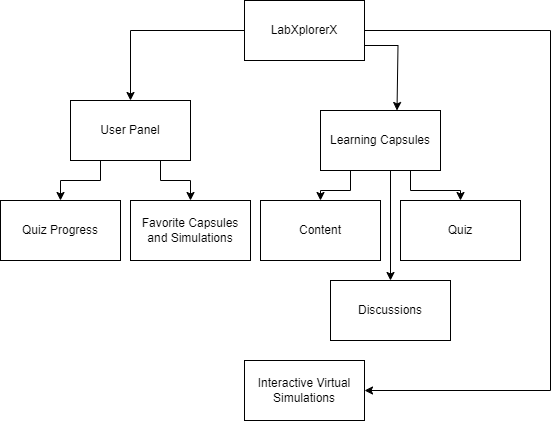
\includegraphics[height = 5.7cm]{Diagrams/Main_Block.png}
    \caption{Main Architecture of System}
\end{figure}
\newpage
\subsection{Data Modelling(ER-Diagram)}
ER Diagram is mainly used to design database schema. With the help of below er diagram we can easily design database in SQL.
\begin{figure}[H]
    \rotatebox{90}{
    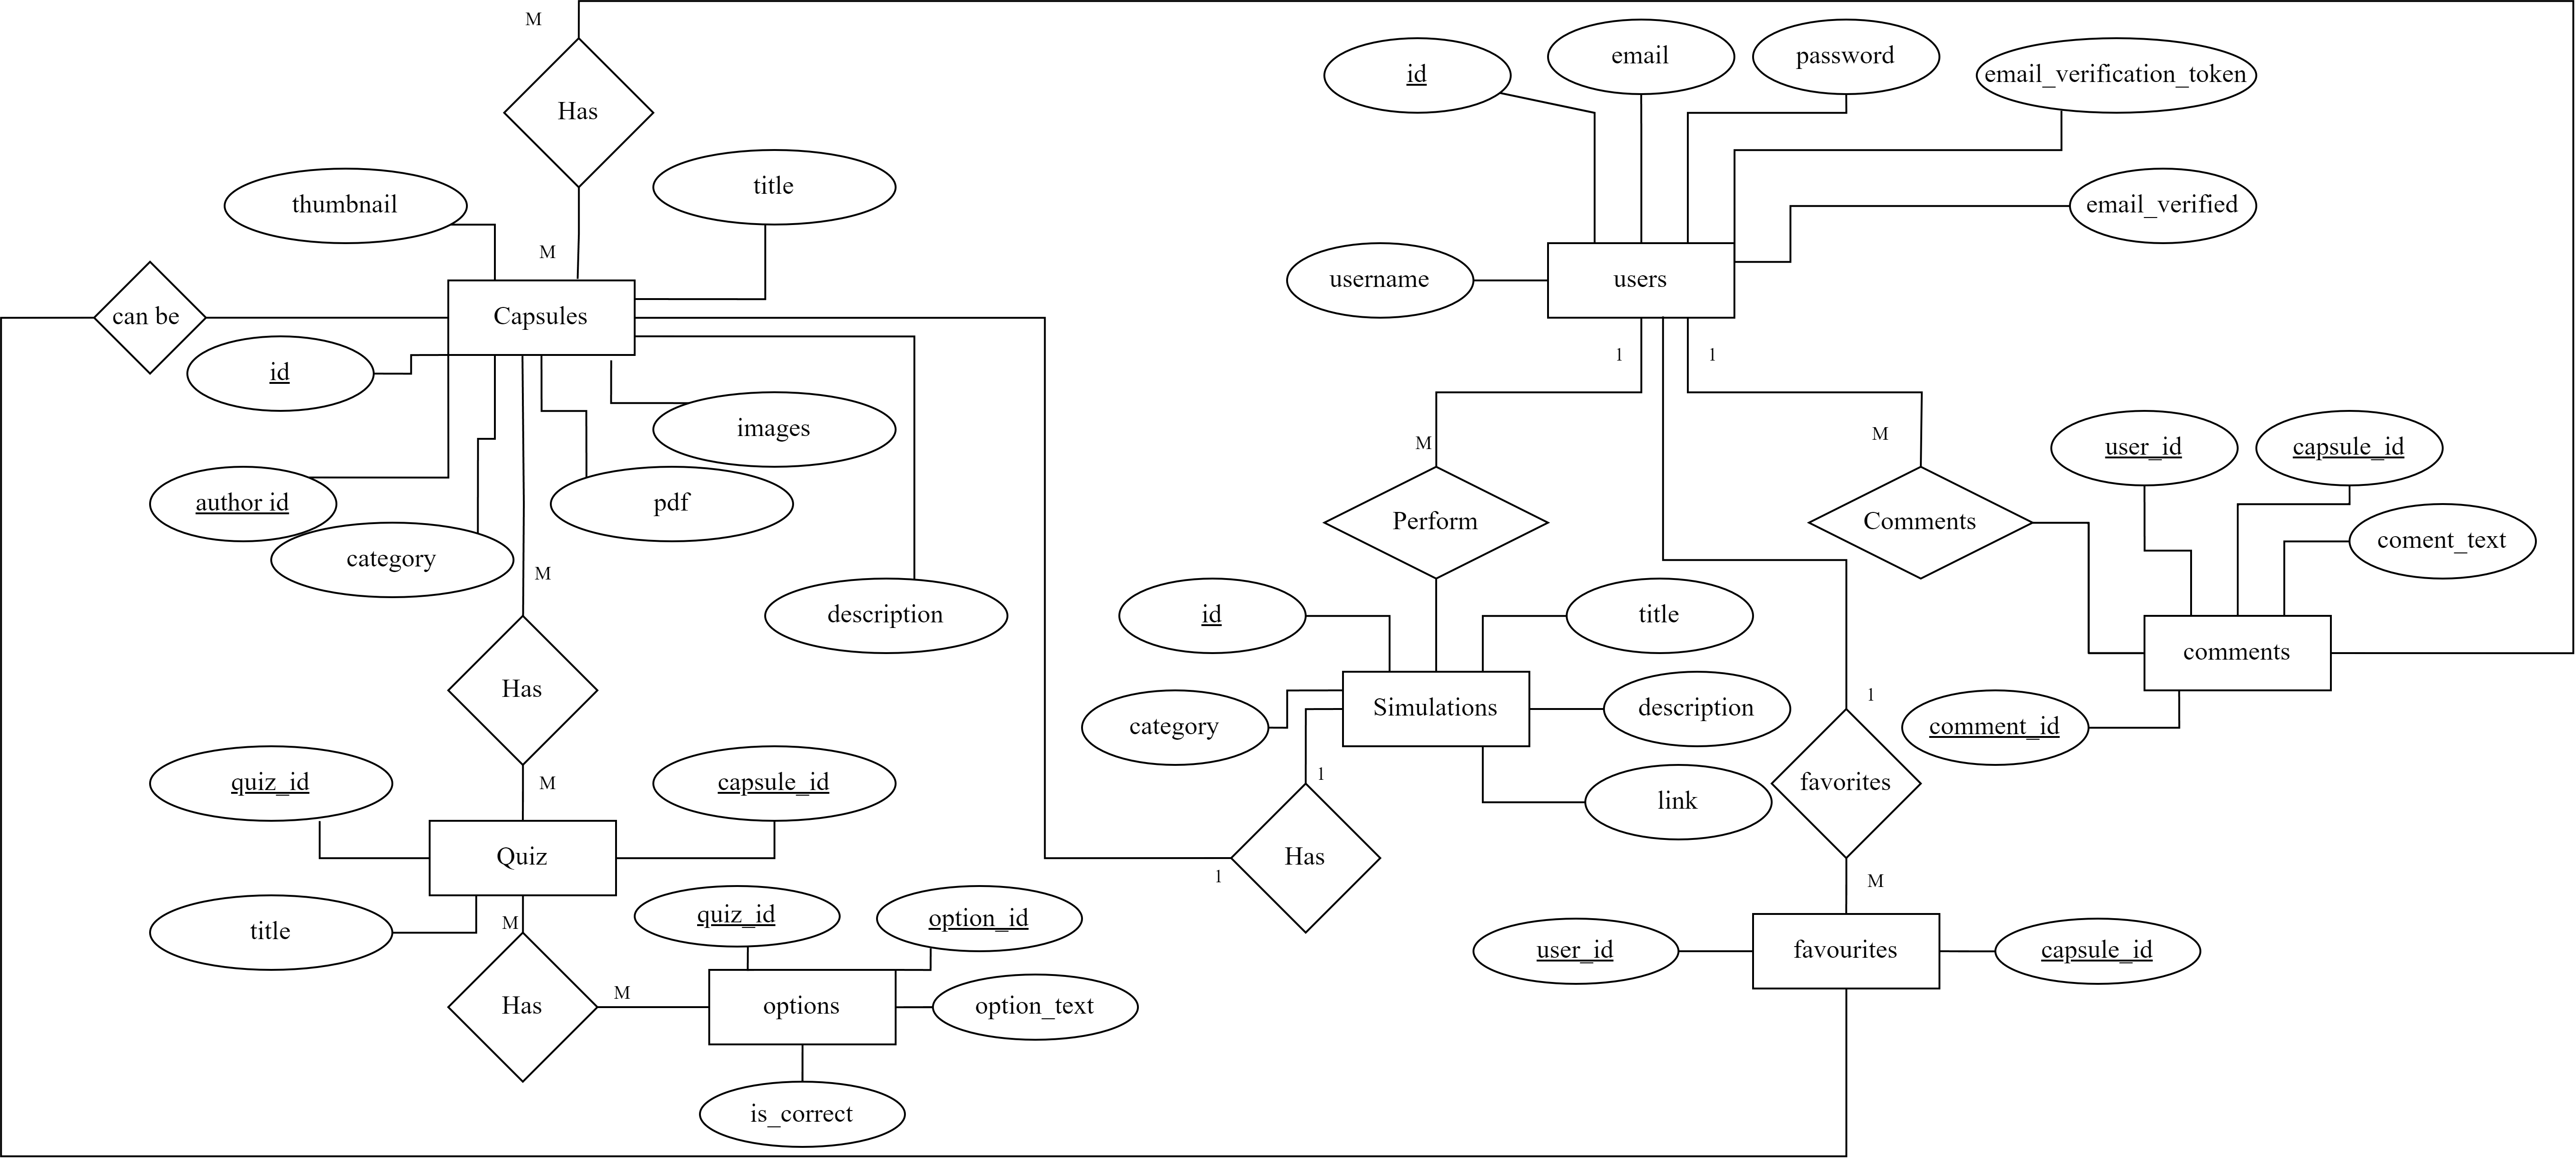
\includegraphics[height = 14cm]{Diagrams/er.drawio.png}}
    \caption{ER Diagram of System Data}
\end{figure}
\newpage
\subsection{Activity Diagram}
An activity diagram visually presents a series of actions or flow of control in a system similar to a flowchart or a data flow diagram. This diagram showed how our program flow goes on.
\begin{figure}[H]
   \centering
    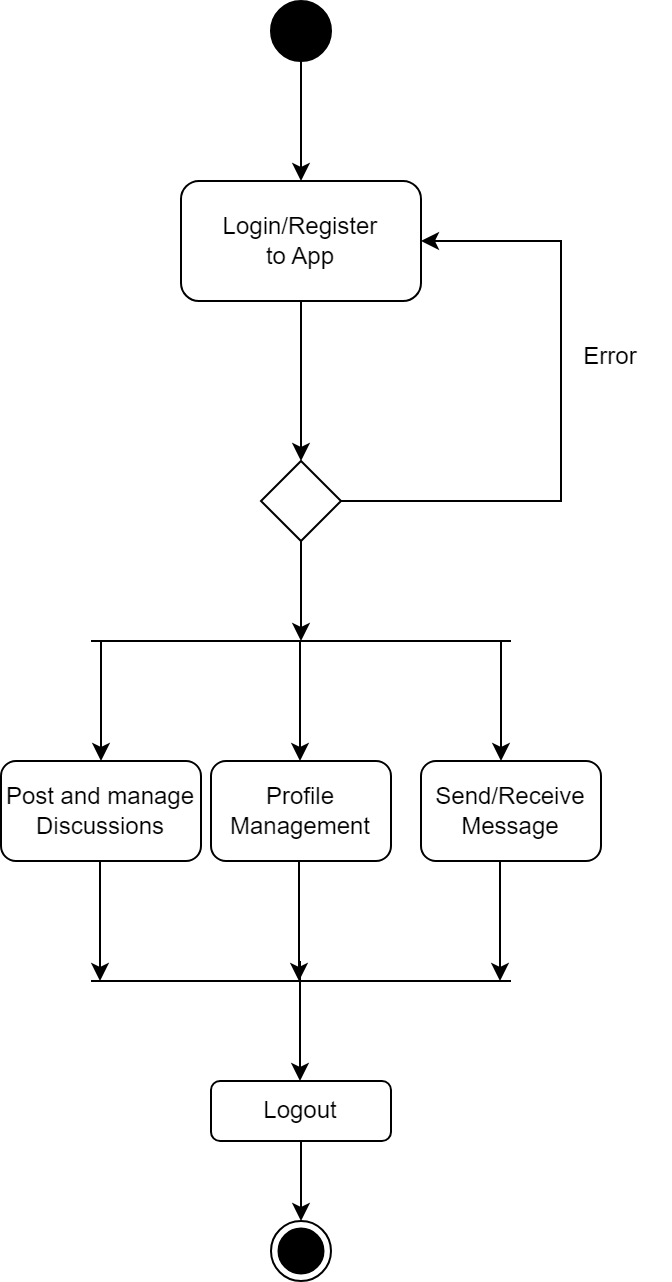
\includegraphics[height = 15cm]{Diagrams/Activity.drawio.png}
    \caption{Activity Diagram}
\end{figure}
\newpage
\subsection{DFD}
DFD or Data Flow Diagram is mainly used to show how data are being flowed in and out of our system. There are 3 levels of DFD i.e Context Level(Level 0),Level 1 and Level 2
\begin{figure}[H]
    \centering
    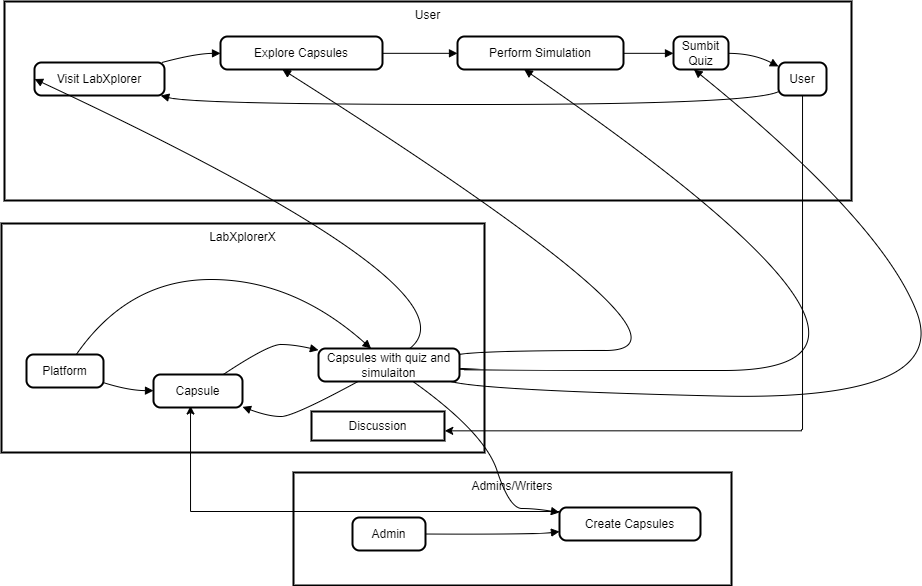
\includegraphics[height = 9cm]{Diagrams/DFD.drawio.png}
    \caption{Data Flow Diagram (Context Level)}
\end{figure}
\newpage
% \subsection{Use Case Diagram}
% A use case diagram, part of UML, visually represents interactions between actors and a system. Actors are external entities, while use cases depict specific functionalities. Relationships, such as association, generalization, include, and extend, illustrate connections between actors and use cases. The diagram helps in understanding system behavior, requirements, and scope.
% \begin{figure}[H]
%     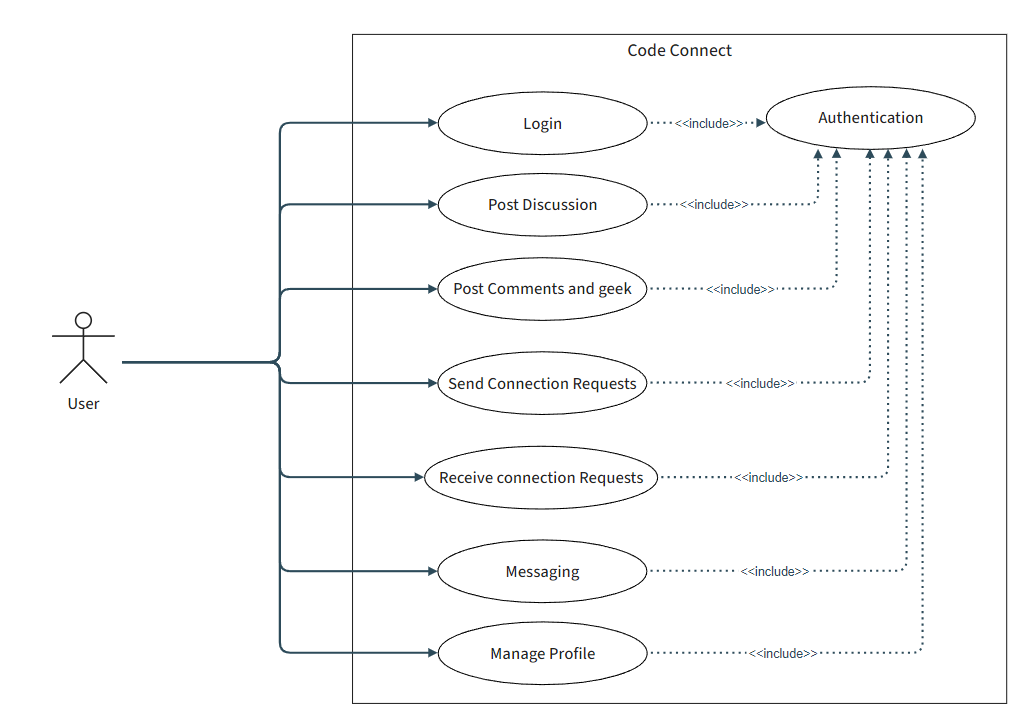
\includegraphics[height = 10cm]{Diagrams/use_case.png}
%     \caption{Use Case Diagram}
% \end{figure}

\chapter{IMPLEMENTATION}


% (20\% of Report Length)

% a. Showcase the output at various intermediate stages of the project pipeline

% b. Use proper data visualizing techniques to present the output

% c. Figures and tables must be accompanied by an explanation
\section{Tools Used}
\textbf{Figma}\\
Figma is a cloud-based design and prototyping tool that empowers teams to collaborate on UI/UX design projects in real-time. It offers a user-friendly interface and powerful features that make it a popular choice among designers. With Figma, designers can create and share interactive prototypes, design components, and design systems. Its cloud-based nature allows for seamless collaboration, enabling multiple team members to work on the same design simultaneously. Figma supports version control, ensuring that design iterations can be easily tracked and managed. \\
\textbf{React}\\
React is a widely-used open-source JavaScript library developed by Facebook for building user interfaces, particularly single-page applications where data changes frequently. It emphasizes a component-based architecture, allowing developers to create reusable UI components that encapsulate their own structure, logic, and styling. React’s use of a virtual DOM enhances performance by minimizing direct updates to the real DOM, ensuring efficient rendering. With its declarative approach, developers specify what the UI should look like based on different states, making the code more predictable and easier to debug. Additionally, React introduces JSX, a syntax extension that combines JavaScript and HTML, making it straightforward to write and understand UI components.\\
\textbf{Postgres}\\
PostgreSQL, often referred to simply as Postgres, is a powerful open-source relational database management system known for its reliability, robustness, and extensibility. Developed over decades and maintained by a global community of contributors, PostgreSQL offers a comprehensive set of features for managing structured data. It supports complex queries, transactions with ACID (Atomicity, Consistency, Isolation, Durability) properties, and a wide range of data types including JSON, XML, and spatial data. PostgreSQL's commitment to standards compliance and continuous improvement ensures compatibility with various programming languages and frameworks. With capabilities for scalability, data integrity, and advanced indexing, PostgreSQL is a preferred choice for applications requiring robust data management and high availability, contributing to its widespread adoption aweb industries from small startups to large enterprises. \\
\textbf{Git/Github}\\
Git is a distributed version control system that is both free and open-source, designed to handle projects of all sizes efficiently and swiftly. It simplifies collaboration by enabling multiple individuals to contribute changes that can be seamlessly merged into a single source. When using Git, the software runs locally on your computer, storing your files and their complete history. Alternatively, you can utilize online hosts like GitHub to store a copy of your files and their revision history. This central repository allows you to easily upload your changes and download updates from other developers, promoting seamless collaboration. Git facilitates automatic merging of changes, allowing multiple individuals to work on different sections of the same file and later merge their modifications without losing any work.\\
\textbf{Node Js with Express}\\
Node.js with Express.js is a powerful combination for building scalable and efficient web applications. Node.js provides a runtime environment that allows JavaScript to be executed server-side, leveraging its event-driven, non-blocking I/O model to handle multiple concurrent connections efficiently. Express.js, as a minimalist web framework for Node.js, simplifies the creation of APIs and routes, offering robust features such as middleware support, routing, and template engines. Together, Node.js and Express.js enable rapid development of RESTful APIs and web servers, making them well-suited for creating real-time applications, microservices, and backend systems. With a vibrant ecosystem of libraries and active community support, Node.js with Express.js remains a popular choice for developers seeking flexibility, performance, and scalability in web application development.\\
\textbf{JavaScript}\\
JavaScript is a programming language that is used to create interactive web pages and backend server. It is a powerful and versatile language that can be used to do a wide variety of things, including adding animation and interactivity to web pages, validating form data, processing user input, making Ajax requests to the server, and creating games and other interactive applications.\\
\textbf{Phaser}\\
Phaser is a powerful and popular open-source HTML5 game framework designed for creating 2D games that can run in both web browsers and mobile environments. Developed by Photon Storm, Phaser is known for its versatility and ease of use, making it a favorite among both beginner and experienced game developers. The framework supports Canvas and WebGL rendering, automatically selecting the best option based on the device's capabilities. Phaser offers a robust set of features including physics engines (Arcade Physics, P2 Physics, and Matter.js), input handling, asset management, animations, and audio integration. Its component-based architecture allows developers to build complex games by combining reusable pieces of code, enhancing modularity and maintainability. With an active community, extensive documentation, and numerous tutorials, Phaser provides ample resources for learning and development, empowering creators to bring their game ideas to life efficiently.
\section*{Postman}
Postman is a widely-used collaboration platform for API development, enabling developers to design, test, document, and monitor APIs with ease. Originally starting as a simple Chrome extension, Postman has evolved into a comprehensive tool that supports the entire API lifecycle. Its intuitive interface allows developers to construct and send HTTP requests to interact with APIs, receiving detailed responses to inspect and debug.

\section*{Unity 3D}
Unity 3D is a leading game development platform renowned for its ability to create both 2D and 3D interactive experiences across a wide range of platforms, including consoles, mobile devices, and VR/AR environments. Developed by Unity Technologies, the engine offers a comprehensive suite of tools that cater to every aspect of game development, from design and prototyping to final deployment.
Unity’s real-time rendering capabilities, coupled with its powerful physics engine, allow developers to create highly immersive and visually stunning games. The engine's support for WebGL enables developers to deploy their games directly to the web, providing browser-based experiences without the need for plugins. WebGL in Unity leverages the engine's advanced rendering capabilities, allowing developers to create complex 3D environments that run smoothly in any modern browser. This makes Unity a versatile tool not only for traditional game development but also for creating interactive web applications.


\subsection{Implementation Details of Modules}
This subsection outlines the implementation specifics for each module, detailing the core functionalities and algorithms utilized. It covers the programming languages, frameworks, and tools used in development, along with the interaction and communication between modules. Key design patterns, data management strategies, and error-handling mechanisms are discussed to ensure optimal performance. Additionally, security measures and optimizations applied during implementation are highlighted.
\newline
\newline
\textbf{Authentication Module}
\newline
The Authentication Module utilizes JSON Web Tokens (JWT) for secure user authentication. JWTs are compact, URL-safe tokens that encode user information, including a signature to verify the token's integrity. After a successful login, a JWT is generated and stored in an HTTP-only cookie, preventing unauthorized access via client-side scripts. The module also includes bcrypt hashing for securely storing user credentials and authentication middleware that checks the validity of the JWT on each request, ensuring only authenticated users can access protected resources.
\begin{figure}[H]
   \centering
    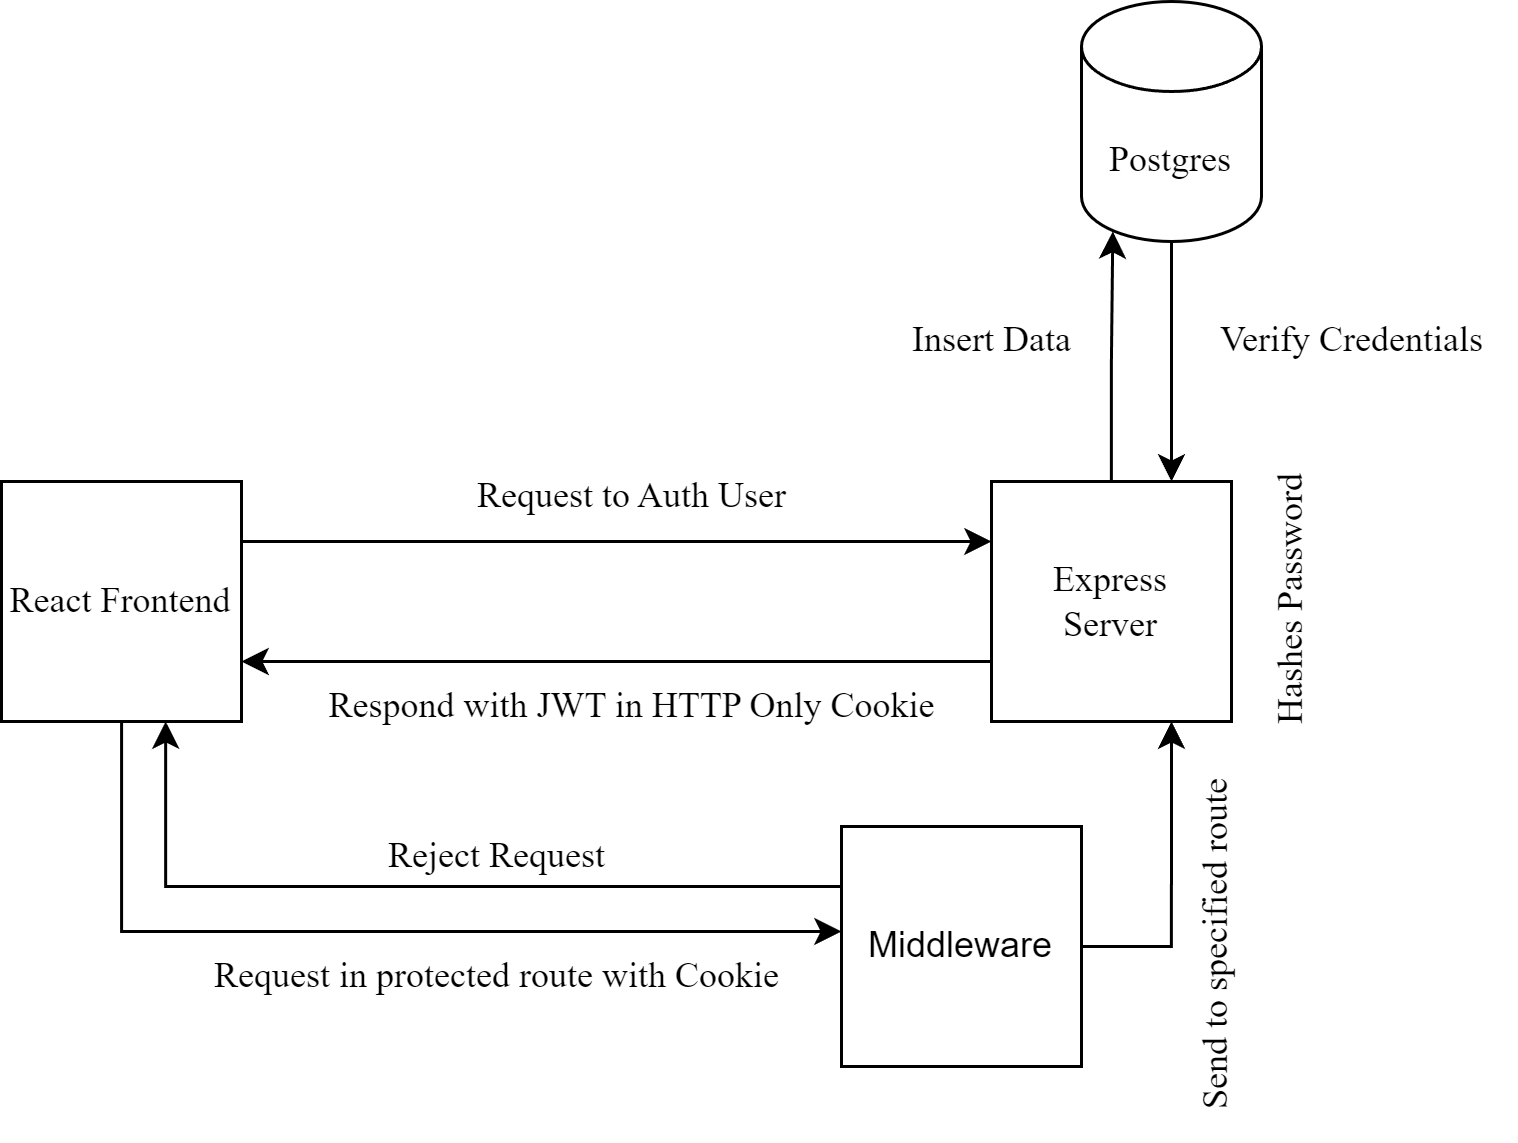
\includegraphics[height = 10cm]{Diagrams/auth module.png}
    \caption{Authnication Module}
\end{figure}
% \subsection{Algorithm Details}
% Here are some of the algorithms of our simulation models:

\subsection{Unit Testing Test Cases}
Theses API unit testing are performed using Postman. API unit testing using Postman involves creating and sending requests to API endpoints to ensure they function correctly. You can write test scripts in Postman to validate responses against expected outcomes, such as status codes and response content. Postman also allows for automating tests using the Collection Runner and Newman for continuous integration and delivery.
\begin{table}[H]
    \caption{Express Endpoint Testing: Capsules GET Methods}
    \label{tab:express_endpoint_testing}
    \resizebox{\textwidth}{!}{%
        \begin{tabular}{|p{0.5in}|p{2.5in}|p{3in}|p{1.5in}|}
            \hline
            \textbf{Test No.} & \textbf{Test Case} & \textbf{Endpoint} & \textbf{ Output} \\
            \hline
            1 & Getting Capsules By Category & \texttt{/api/capsule/category?category\newline=physics} & Returns JSON response with Array of Objects with specific category \\
            \hline
            2 & Getting Capsules By Id & \texttt{/api/capsule/?capsuleId=1} & Returns JSON response with Object of Capsules with specific id  \\
            \hline
            3 & Getting All Capsules & \texttt{/api/capsule/all} & Returns JSON response with Array of Objects of Capsules \\
            \hline
        \end{tabular}%
    }
\end{table}
\begin{table}[H]
    \caption{Express Endpoint Testing: Capsules GET Methods}
    \label{tab:express_endpoint_testing}
    \resizebox{\textwidth}{!}{%
        \begin{tabular}{|p{0.5in}|p{2.5in}|p{3in}|p{1.5in}|}
            \hline
            \textbf{Test No.} & \textbf{Test Case} & \textbf{Endpoint} & \textbf{ Output} \\
            \hline
            1 & Login user/admin endpoint & \texttt{/api/user/login\newline body: Username and Password} & Creates JWT token and sets an HTTP Only Cookie to the client side \\
            \hline
            2 & api/user/register & \texttt{/api/capsule/category?category\newline=physics} & Returns JSON response with Array of Objects with id \\
            \hline
           
        \end{tabular}%
    }
\end{table}
\begin{table}[H]
    \caption{Express Endpoint Testing: User Methods}
    \label{tab:express_endpoint_testing}
    \resizebox{\textwidth}{!}{%
        \begin{tabular}{|p{0.5in}|p{2.5in}|p{3in}|p{1.5in}|}
            \hline
            \textbf{Test No.} & \textbf{Test Case} & \textbf{Endpoint} & \textbf{ Output} \\
            \hline
            1 & Admin add capsule endpoint & \texttt{api/admin/add\newline body:capsule informations and images} & Sucessfully adds images in uploads folder and corresponding capsule into database  \\
            \hline
            
        \end{tabular}%
    }
\end{table}
\newpage
\subsection{Test Cases for System Testing}
System Testing involves a comprehensive evaluation of the entire PERN application, including both frontend and backend components. This phase aims to validate that all integrated parts of the system function correctly and cohesively. We will test the complete application flow to ensure seamless interaction between the frontend and backend, as well as to verify that the application meets its specified requirements and performs as expected.
\begin{table}[H]
    \caption{System/Application Testing: Capsules GET Methods}
    \label{tab:express_endpoint_testing}
    \resizebox{\textwidth}{!}{%
        \begin{tabular}{|p{0.5in}|p{2.5in}|p{3in}|p{1.5in}|}
            \hline
            \textbf{Test No.} & \textbf{Test Case} & \textbf{Input} & \textbf{ Output} \\
            \hline
            1 & Acessing Specific Capsules By Id & \texttt{/capsule/8\newline} & Shows whole capsule its images, pdf and all its meta information with quiz \\
            \hline
            2 & Acessing Capsules Menu By Category & \texttt{/capsules/physics} & Shows cards, thumbnail, title, description and buttons about related category capsules  \\
            \hline
            3 & Getting All Capsules & \texttt{/learning-area} & Shows Learning Capsules with categories of each capsules \\
            \hline
        \end{tabular}%
    }
\end{table}
\begin{table}[H]
    \caption{System/Application Testing: Login}
    \label{tab:express_endpoint_testing}
    \resizebox{\textwidth}{!}{%
        \begin{tabular}{|p{0.5in}|p{2.5in}|p{3in}|p{1.5in}|}
            \hline
            \textbf{Test No.} & \textbf{Test Case} & \textbf{Input} & \textbf{ Output} \\
            \hline
            1 & Login User & \texttt{/login\newline Input: Username 'test' and Password 'test'} & Creates JWT token and sets an HTTP Only Cookie to the client side and redirects user into profile page\\
            \hline
            1 & Login Admin & \texttt{/login\newline Input: Username 'Admin' and Password 'admin'} & Creates JWT token and sets an HTTP Only Cookie to the client side and redirects user into profile page also shows Admin Button for Admin Panel\\
            \hline
           
        \end{tabular}%
    }
\end{table}
\begin{table}[H]
    \caption{System/Application Testing: User Methods}
    \label{tab:express_endpoint_testing}
    \resizebox{\textwidth}{!}{%
        \begin{tabular}{|p{0.5in}|p{2.5in}|p{3in}|p{1.5in}|}
            \hline
            \textbf{Test No.} & \textbf{Test Case} & \textbf{Input} & \textbf{ Output} \\
            \hline
            1 & Admin add capsule & \texttt{/admin/add} & Shows Form to add capsules and adds capsules when submitted  \\
            \hline
            
        \end{tabular}%
    }
\end{table}
\chapter{CONCLUSION AND ANALYSIS}
\section{Conclusion}
LabXplorerX is an innovative virtual laboratory platform tailored for enhancing science education through interactive simulations and experiments. It aims to revolutionize how students and educators engage with scientific concepts by offering a diverse range of features. LabXplorerX facilitates seamless exploration, collaboration, and learning aweb various scientific disciplines. This platform empowers users to conduct experiments, share insights, and leverage sophisticated algorithms to deepen their understanding. Additionally, LabXplorerX integrates advanced reporting capabilities and decision-making tools, enriching the educational experience beyond traditional classroom settings.
\section{Work Completed}
In the LabXplorerX project, significant strides have been made in creating an engaging and educational platform for students. Five interactive simulations have been successfully developed, offering hands-on learning experiences across various subjects. Additionally, learning capsules have been crafted to provide structured, multimedia-rich content that enhances student understanding. A robust authentication system has been implemented, ensuring secure access for students and teachers. The development of an admin panel enables efficient management of users, content, and simulations, while integrated quizzes allow students to assess their knowledge with immediate feedback.

\begin{itemize}[leftmargin=1cm]
    \item \textbf{Creation of Simulations:} Successfully developed 5 simulations, each tailored to provide interactive and educational experiences for students in various subject areas.
    
    \item \textbf{Learning Capsules:} Created comprehensive learning capsules that include structured content, interactive elements, and visual aids to enhance the learning experience.
    
    \item \textbf{Authentication:} Implemented a robust authentication system to manage user access, including secure login, registration, and account management features for both students and teachers.
    
    \item \textbf{Admin Panel:} Developed an admin panel that allows administrators to manage users, simulations, and content. The panel includes tools for monitoring user progress, updating content, and overseeing the overall platform.
    
    \item \textbf{Quizzes:} Integrated quizzes into the learning modules, enabling students to assess their understanding of the material. The quizzes are designed to be interactive and provide immediate feedback to the learners.
\end{itemize}
\subsection{Screenshots of Outcomes}
\begin{figure}[H]
    \centering
     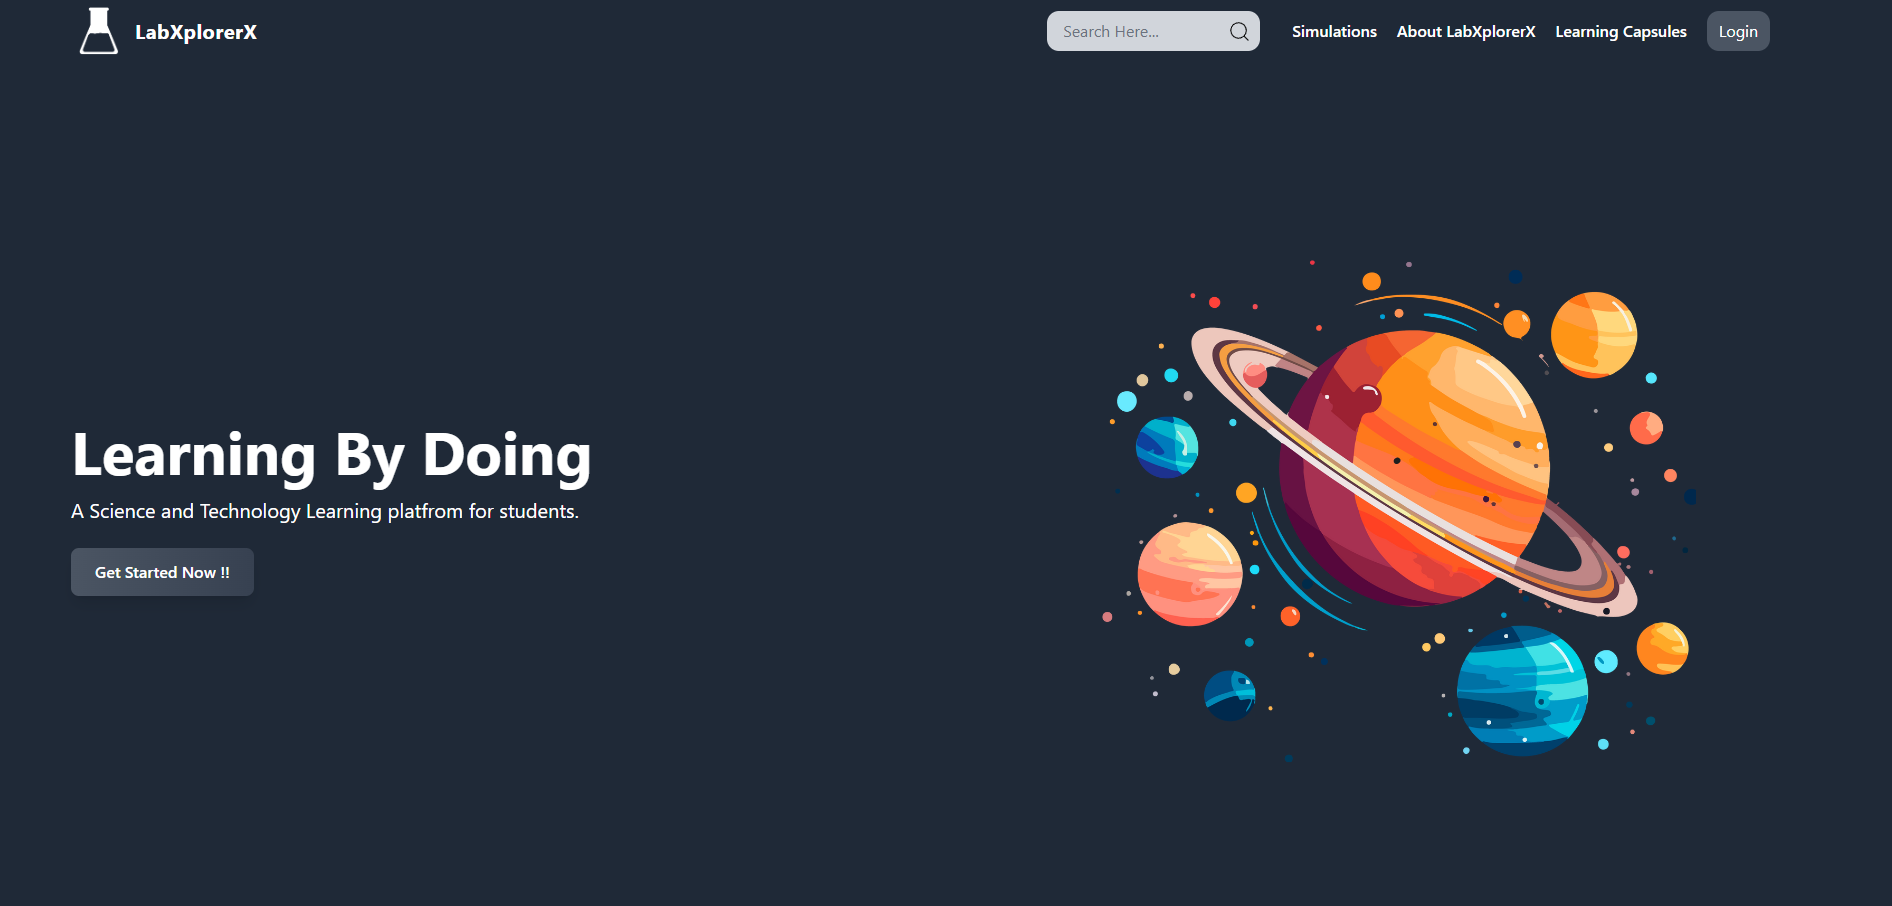
\includegraphics[width = 16cm]{Diagrams/output/home.png}
     \caption{Home Screen}
 \end{figure}

 \begin{figure}[H]
    \centering
     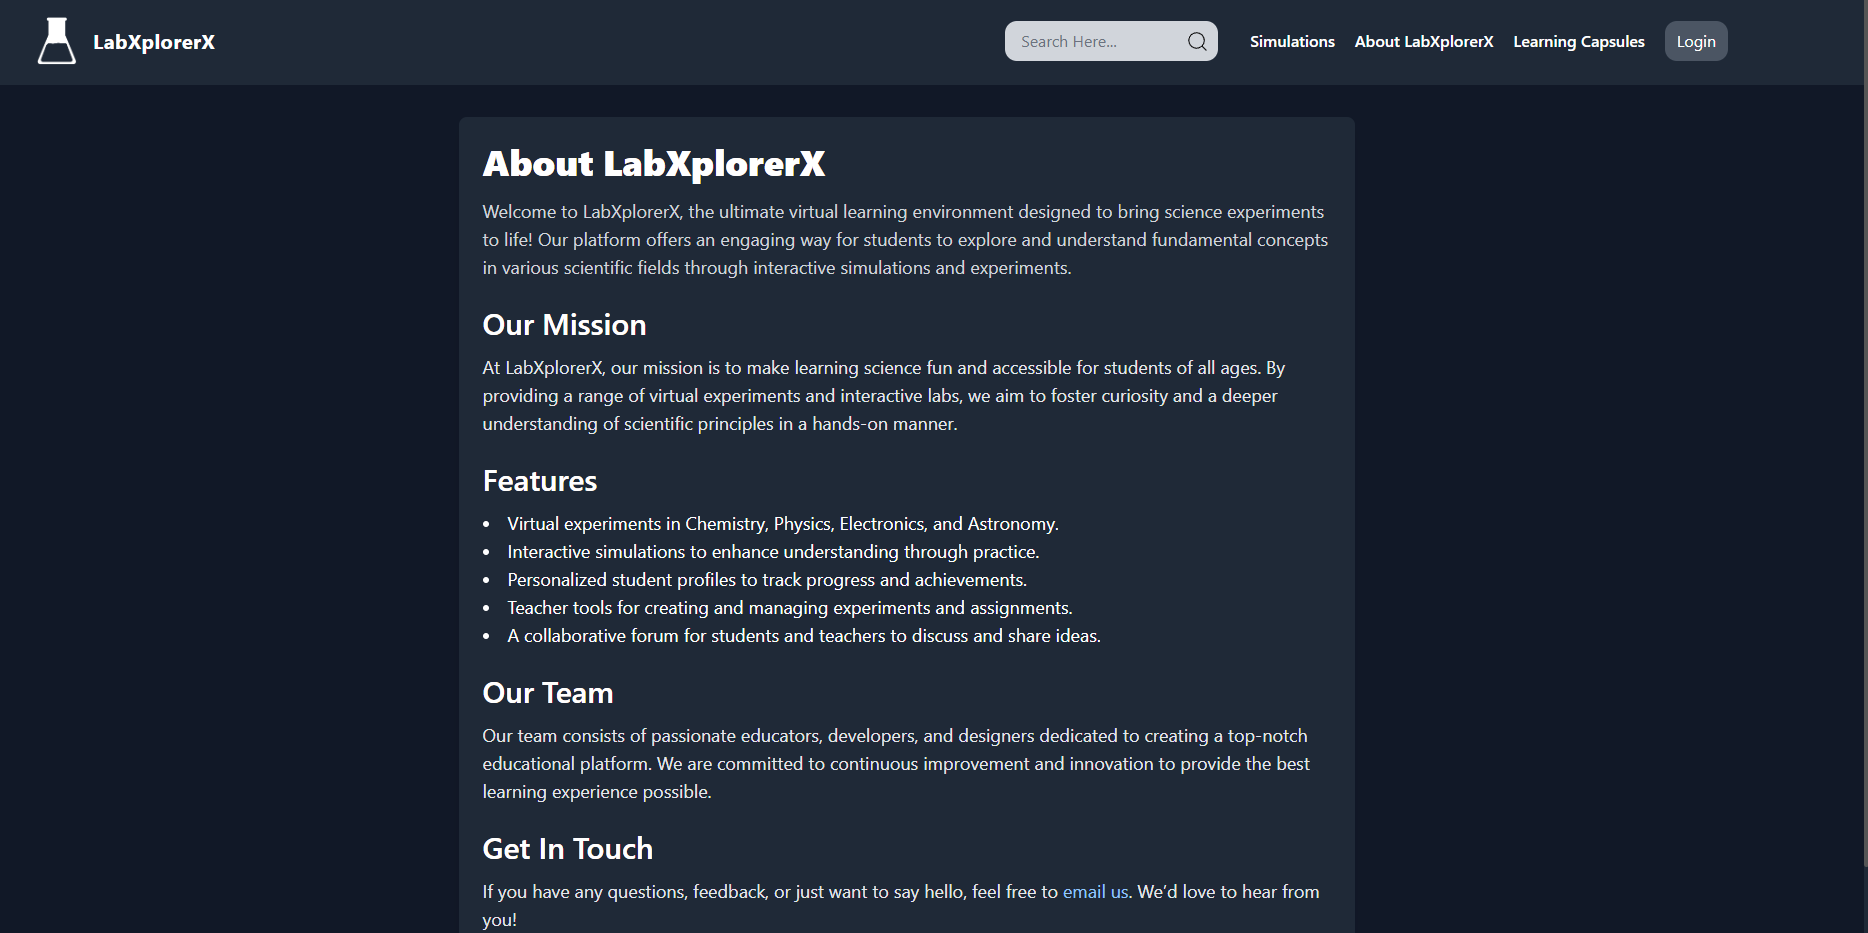
\includegraphics[width = 16cm]{Diagrams/output/about.png}
     \caption{About Page}
 \end{figure}

 \begin{figure}[H]
    \centering
     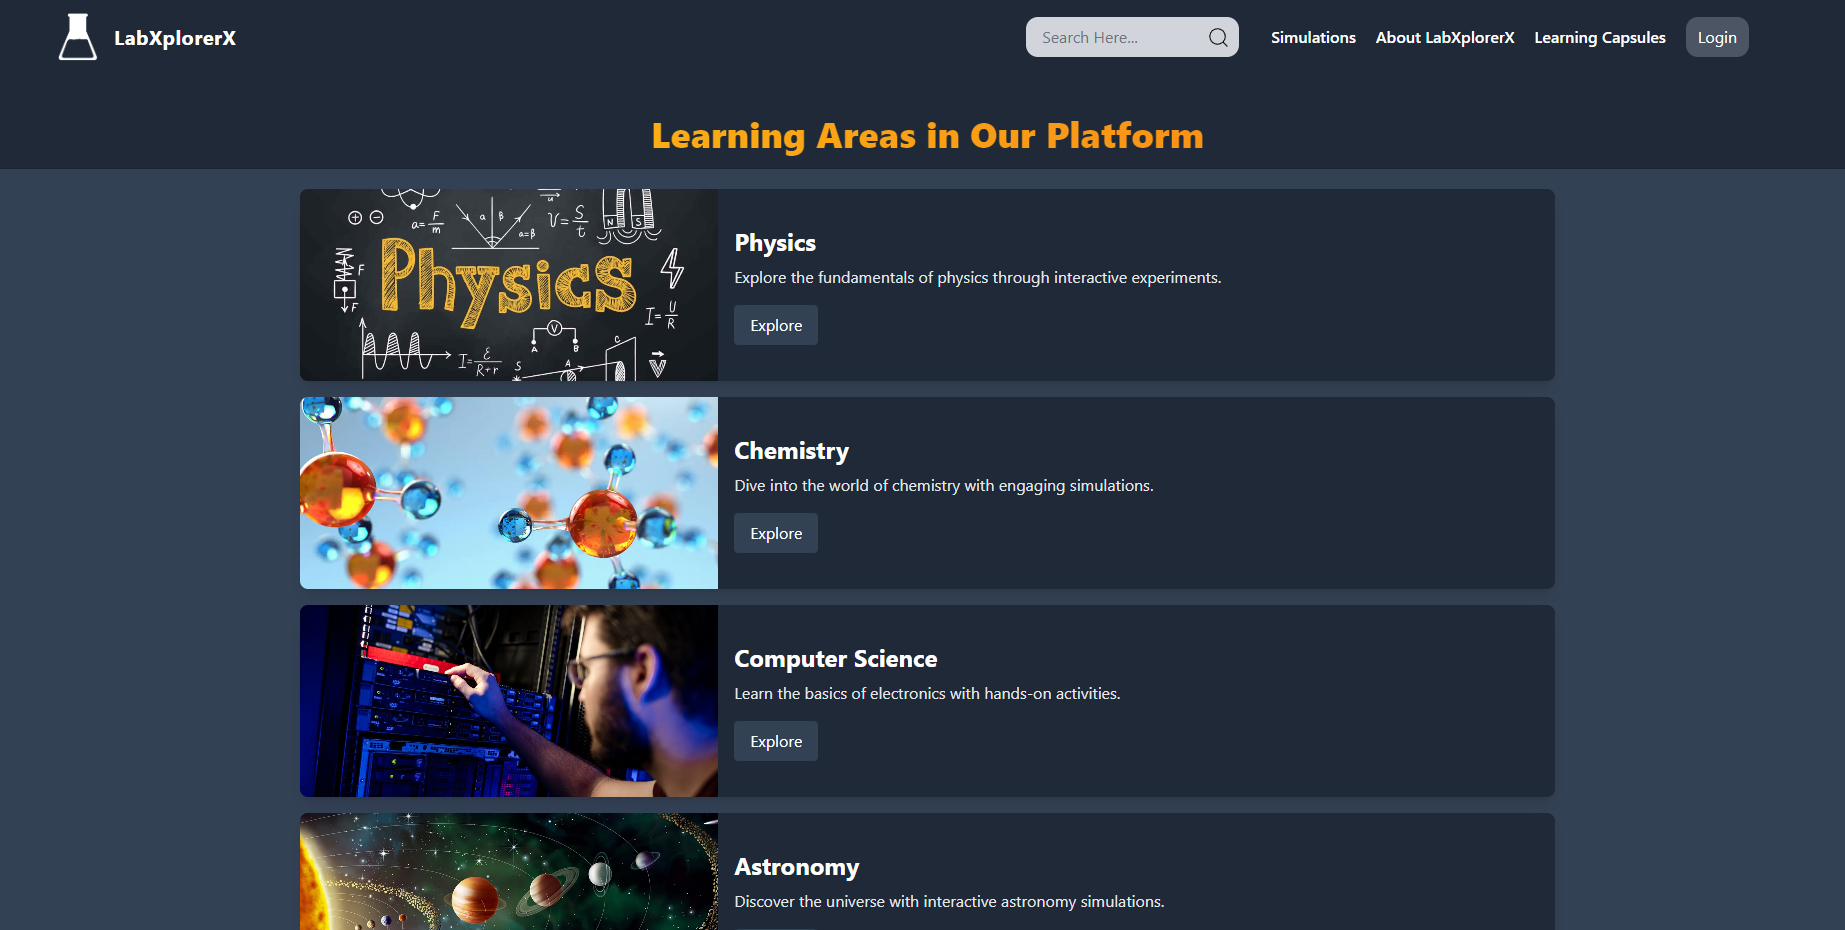
\includegraphics[width = 16cm]{Diagrams/output/learningareas.png}
     \caption{Learning Areas}
 \end{figure}


 \begin{figure}[H]
    \centering
     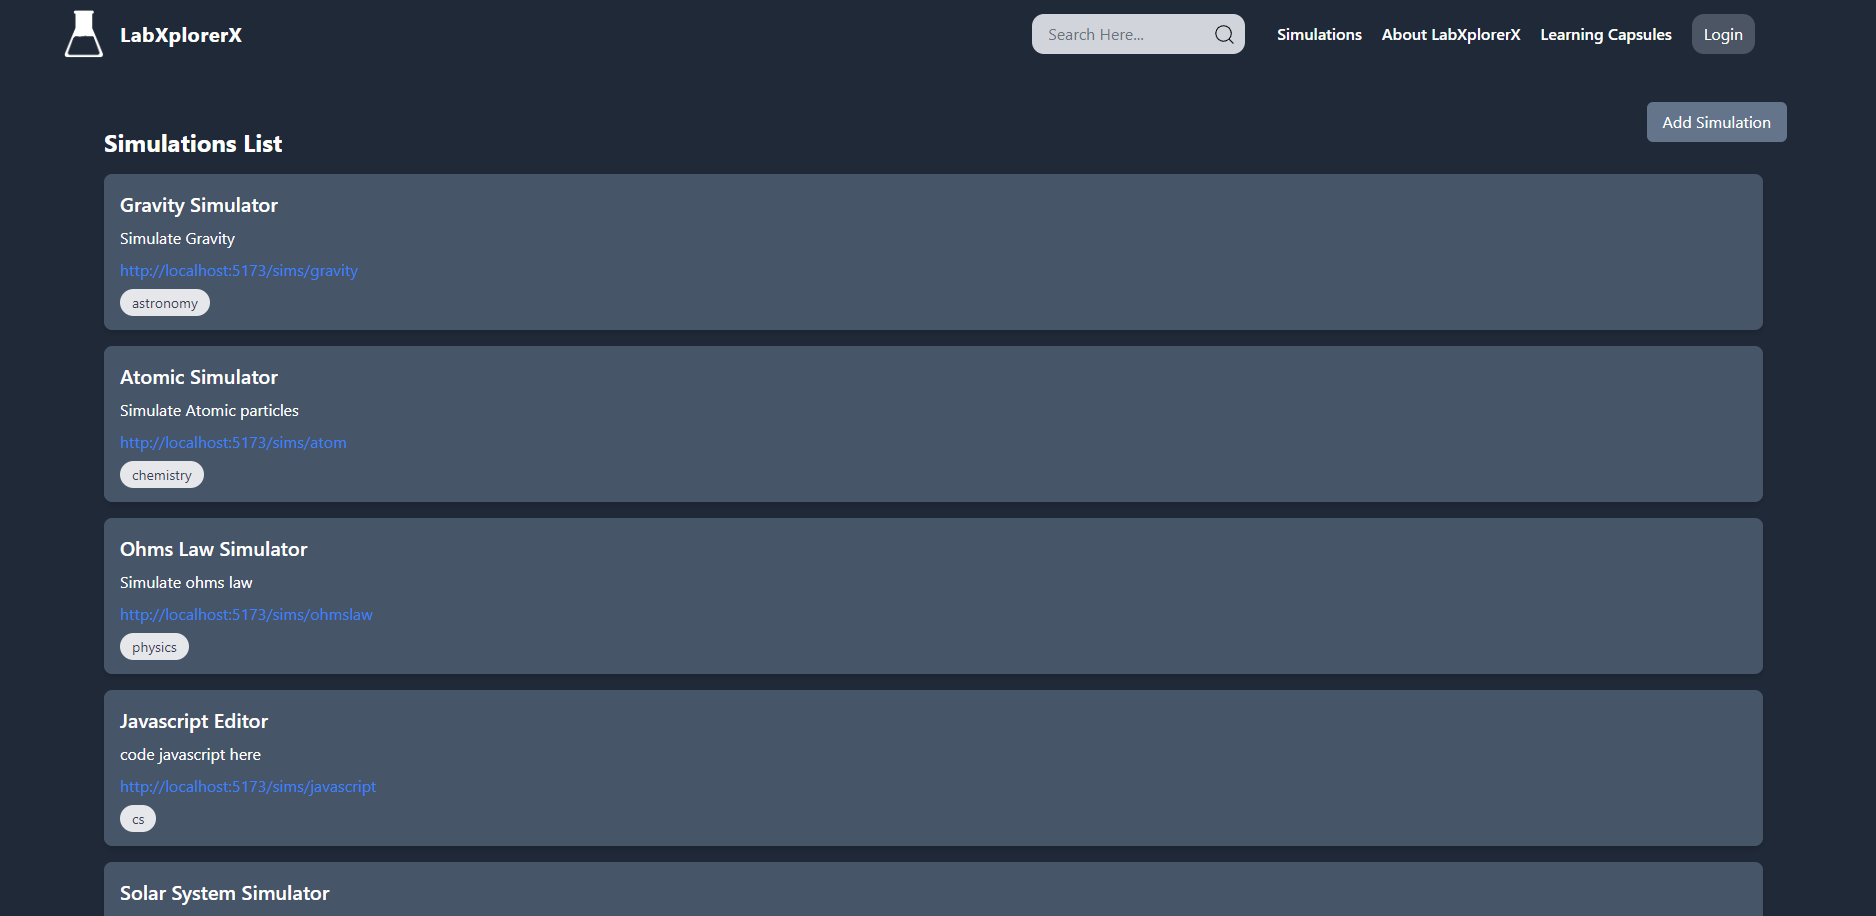
\includegraphics[width = 16cm]{Diagrams/output/simulations.png}
     \caption{Simulations}
 \end{figure}

 \begin{figure}[H]
    \centering
     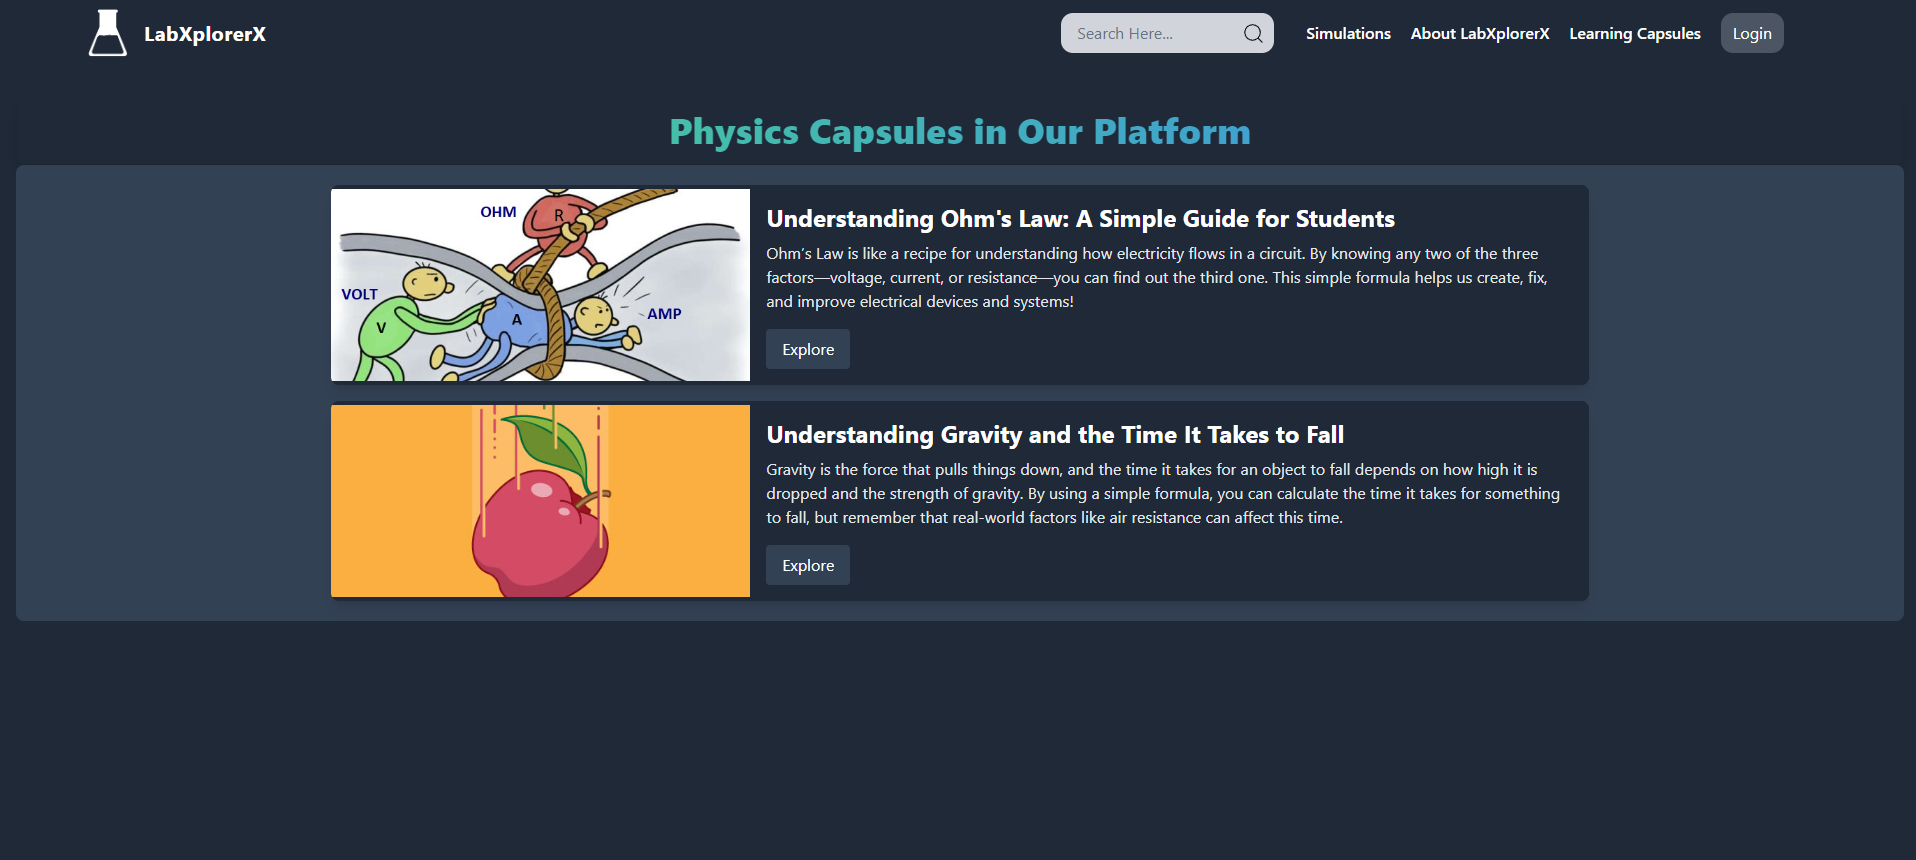
\includegraphics[width = 16cm]{Diagrams/output/capsules.png}
     \caption{Capsules}
 \end{figure}

 \begin{figure}[H]
    \centering
     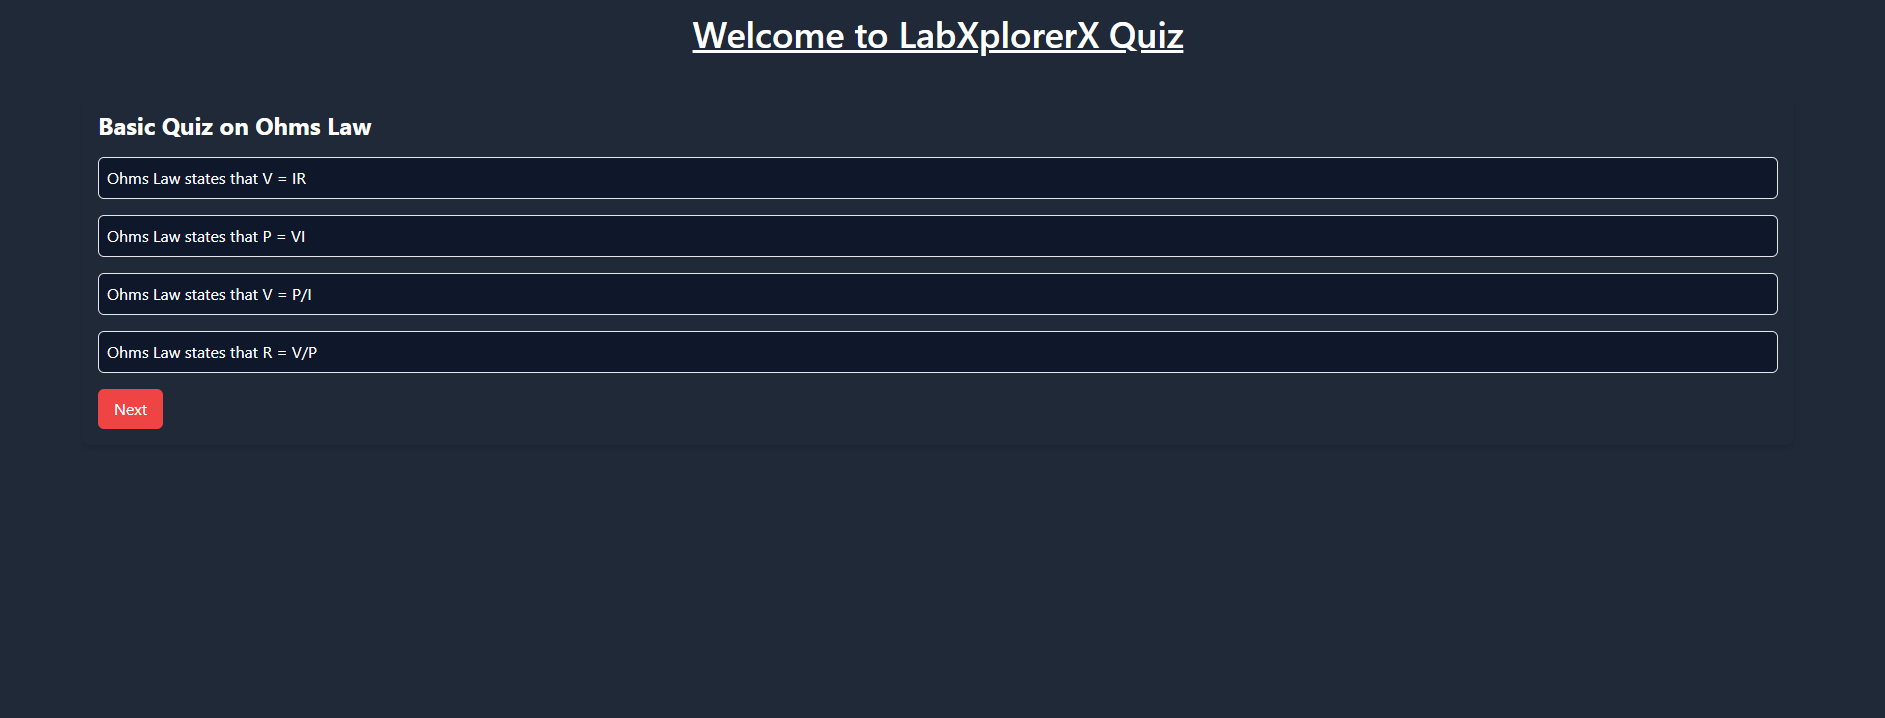
\includegraphics[width = 16cm]{Diagrams/output/quiz.png}
     \caption{Quizzes}
 \end{figure}

 \begin{figure}[H]
    \centering
     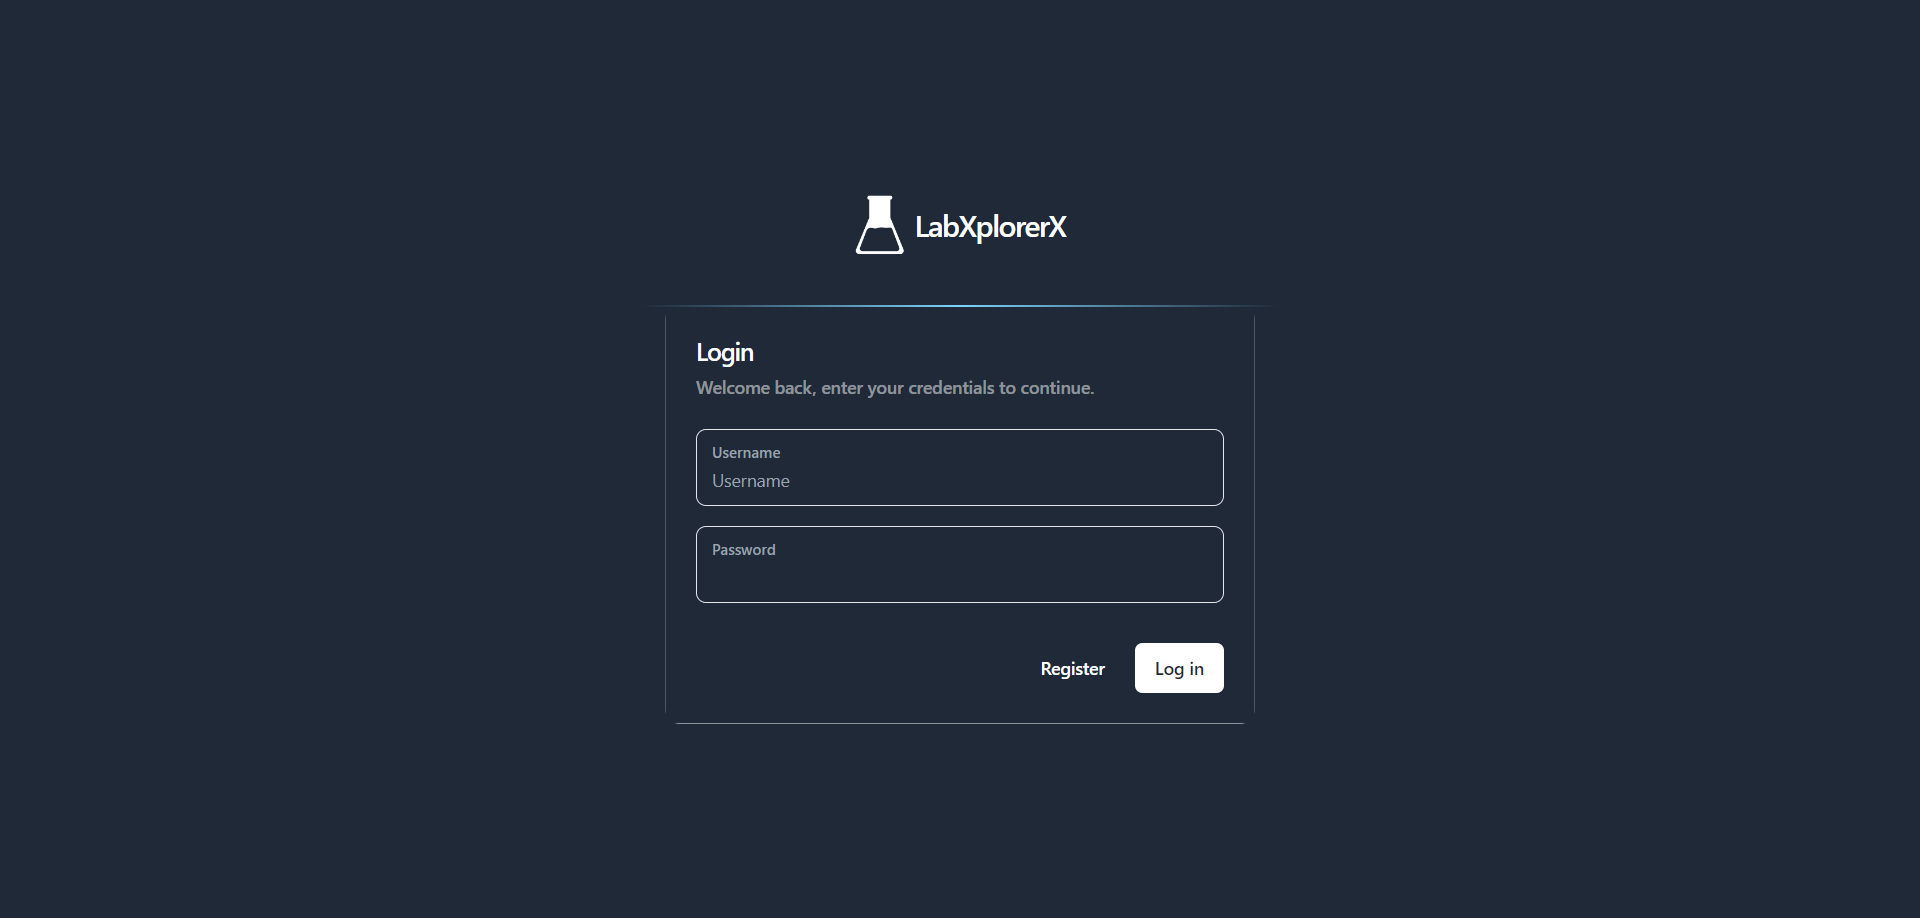
\includegraphics[width = 16cm]{Diagrams/output/login.png}
     \caption{Login}
 \end{figure}

 \begin{figure}[H]
    \centering
     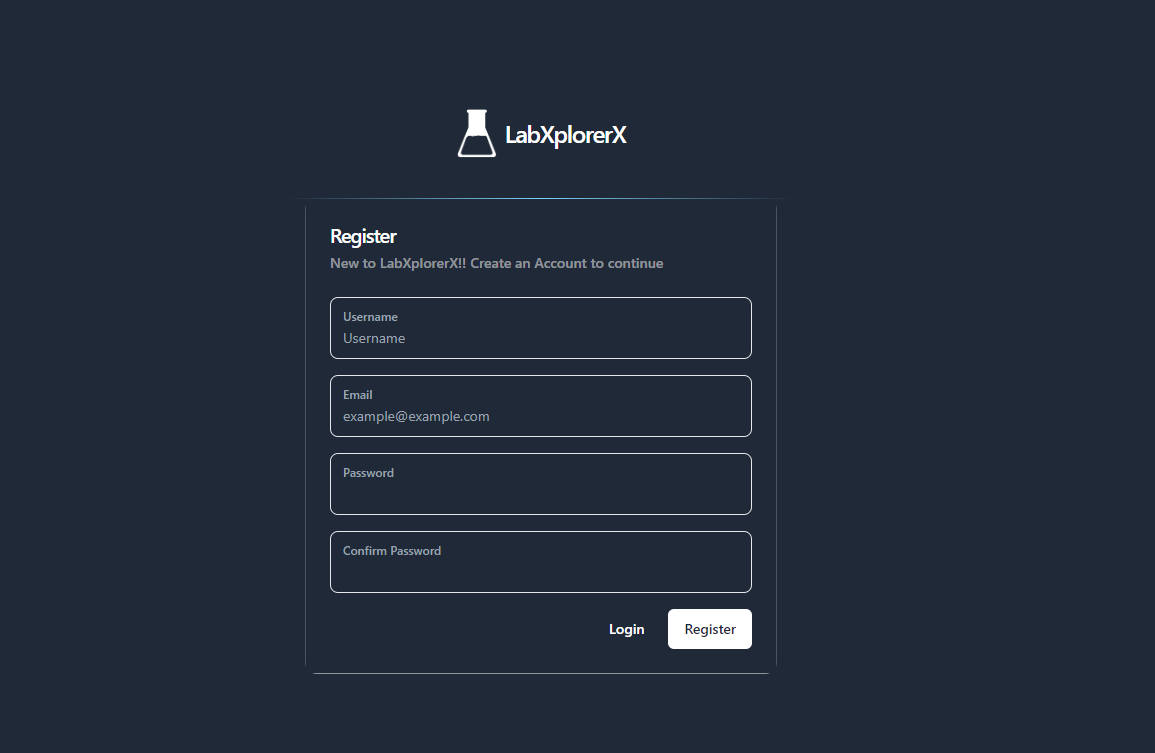
\includegraphics[width = 16cm]{Diagrams/output//register.png}
     \caption{Register}
 \end{figure}

 \begin{figure}[H]
    \centering
     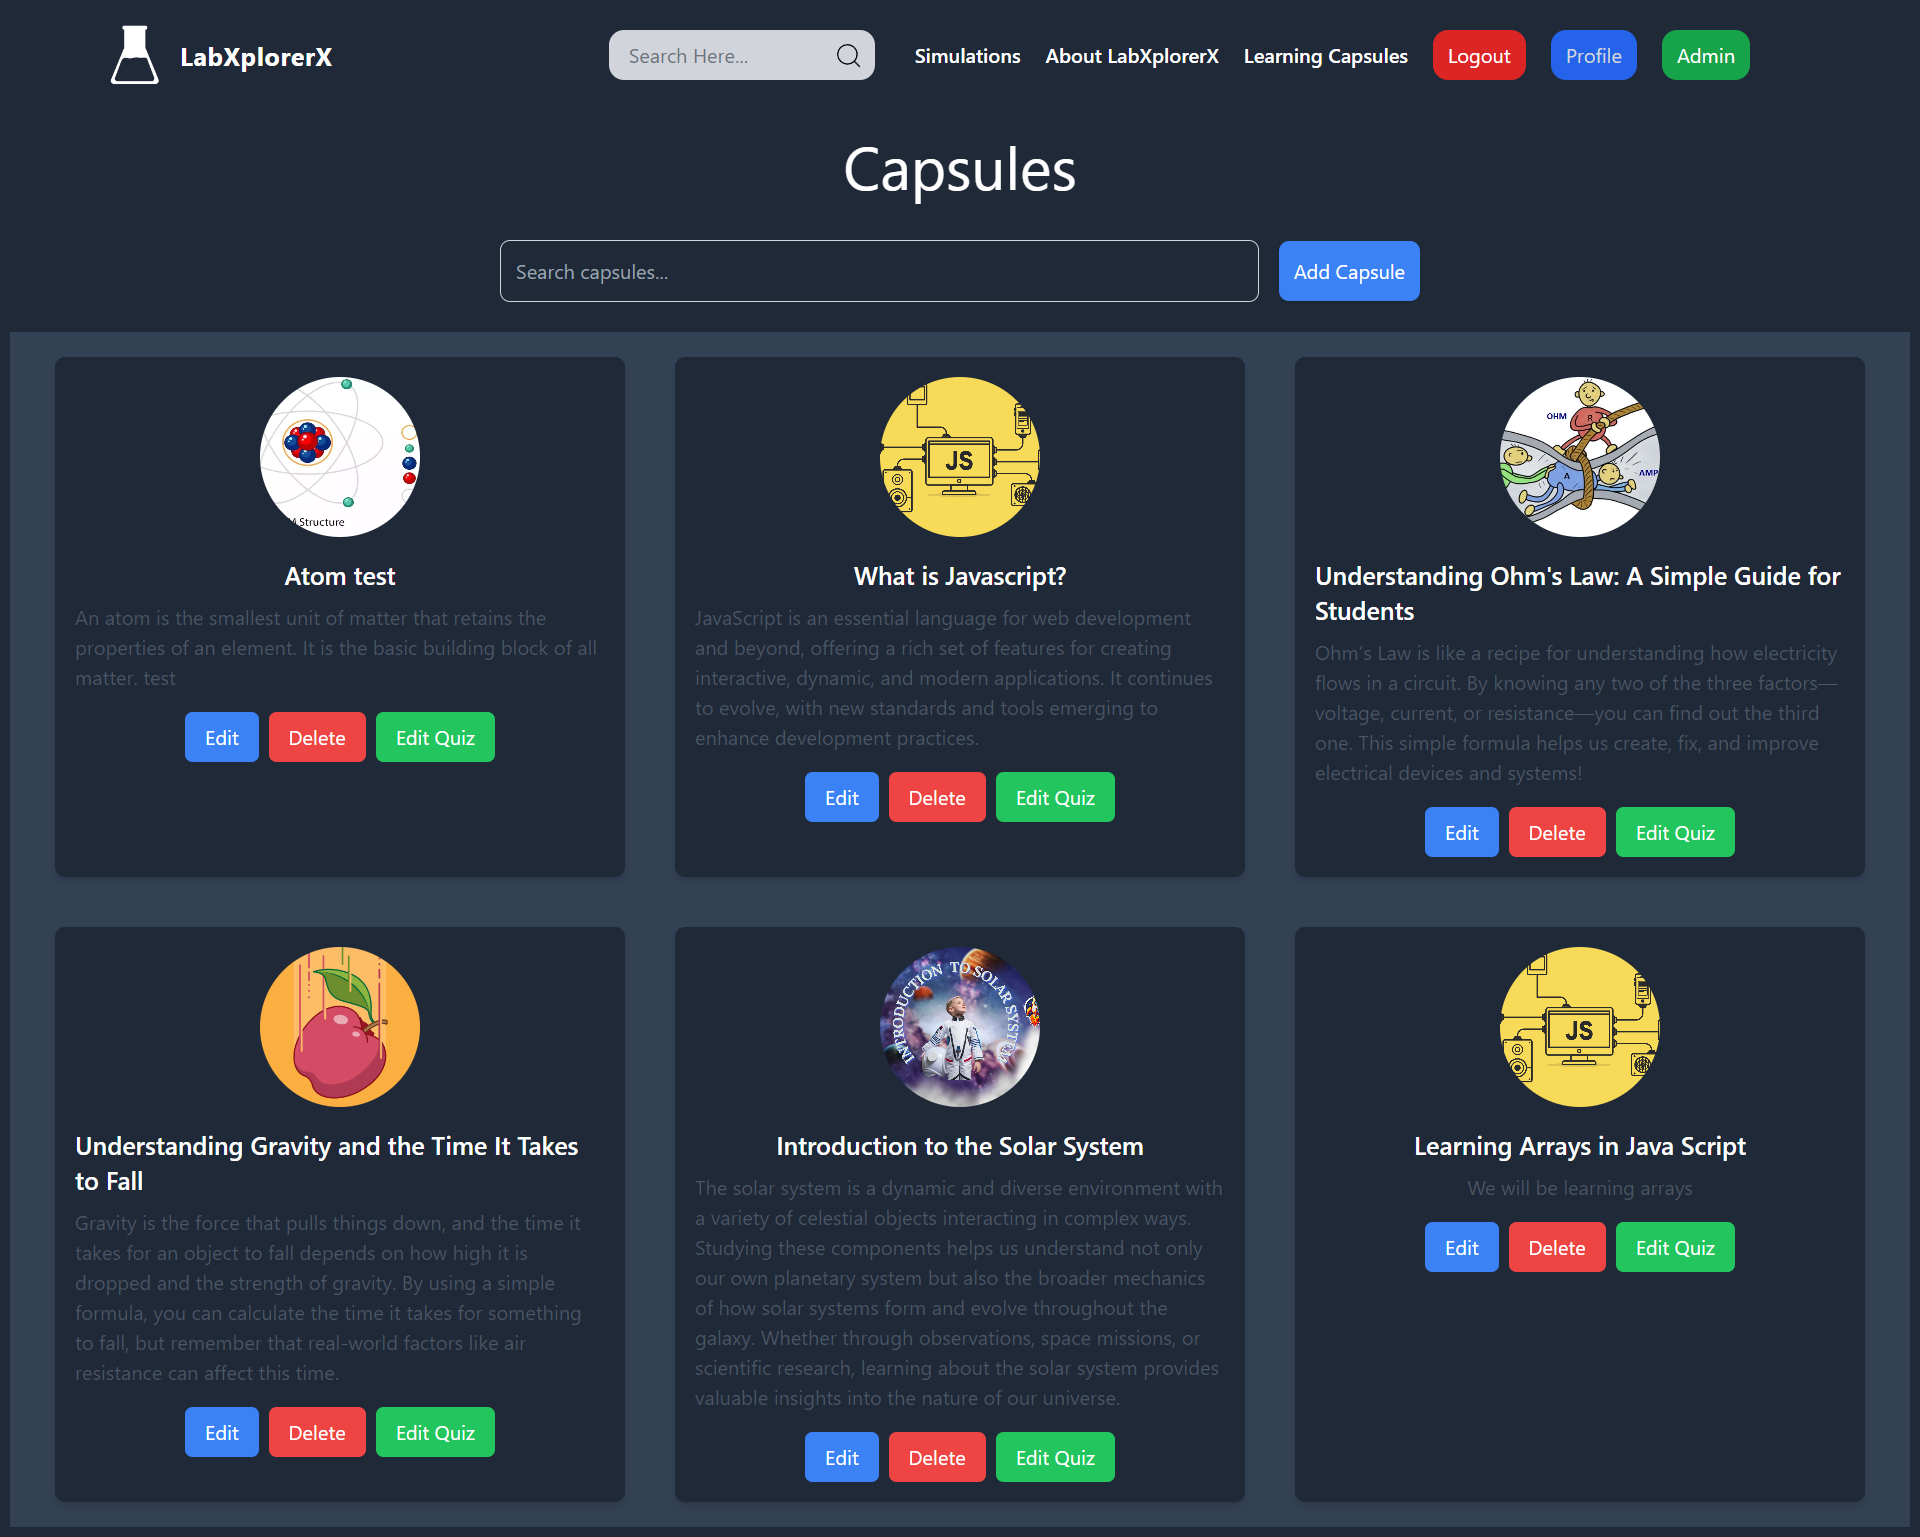
\includegraphics[width = 16cm]{Diagrams/output/admin.png}
     \caption{Admin Panel}
 \end{figure}

 \begin{figure}[H]
    \centering
     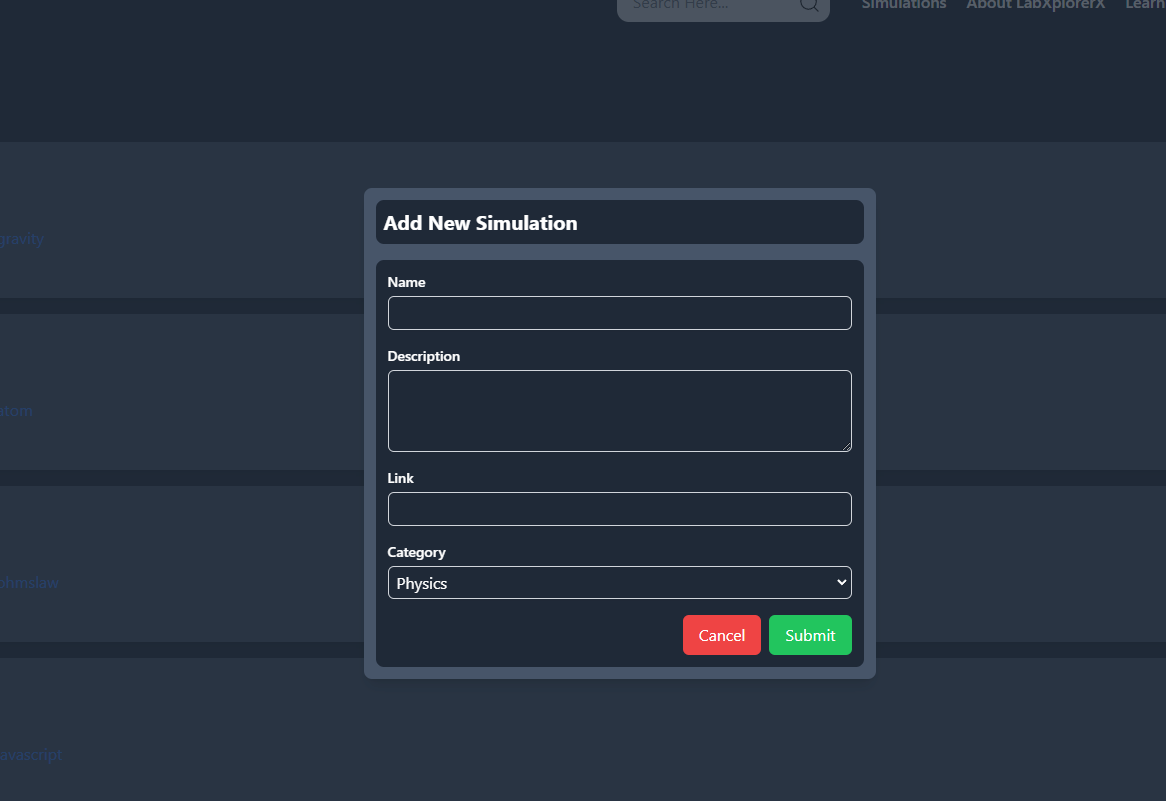
\includegraphics[width = 16cm]{Diagrams/output/addsimulations.png}
     \caption{Add Simulations}
 \end{figure}

 \begin{figure}[H]
    \centering
     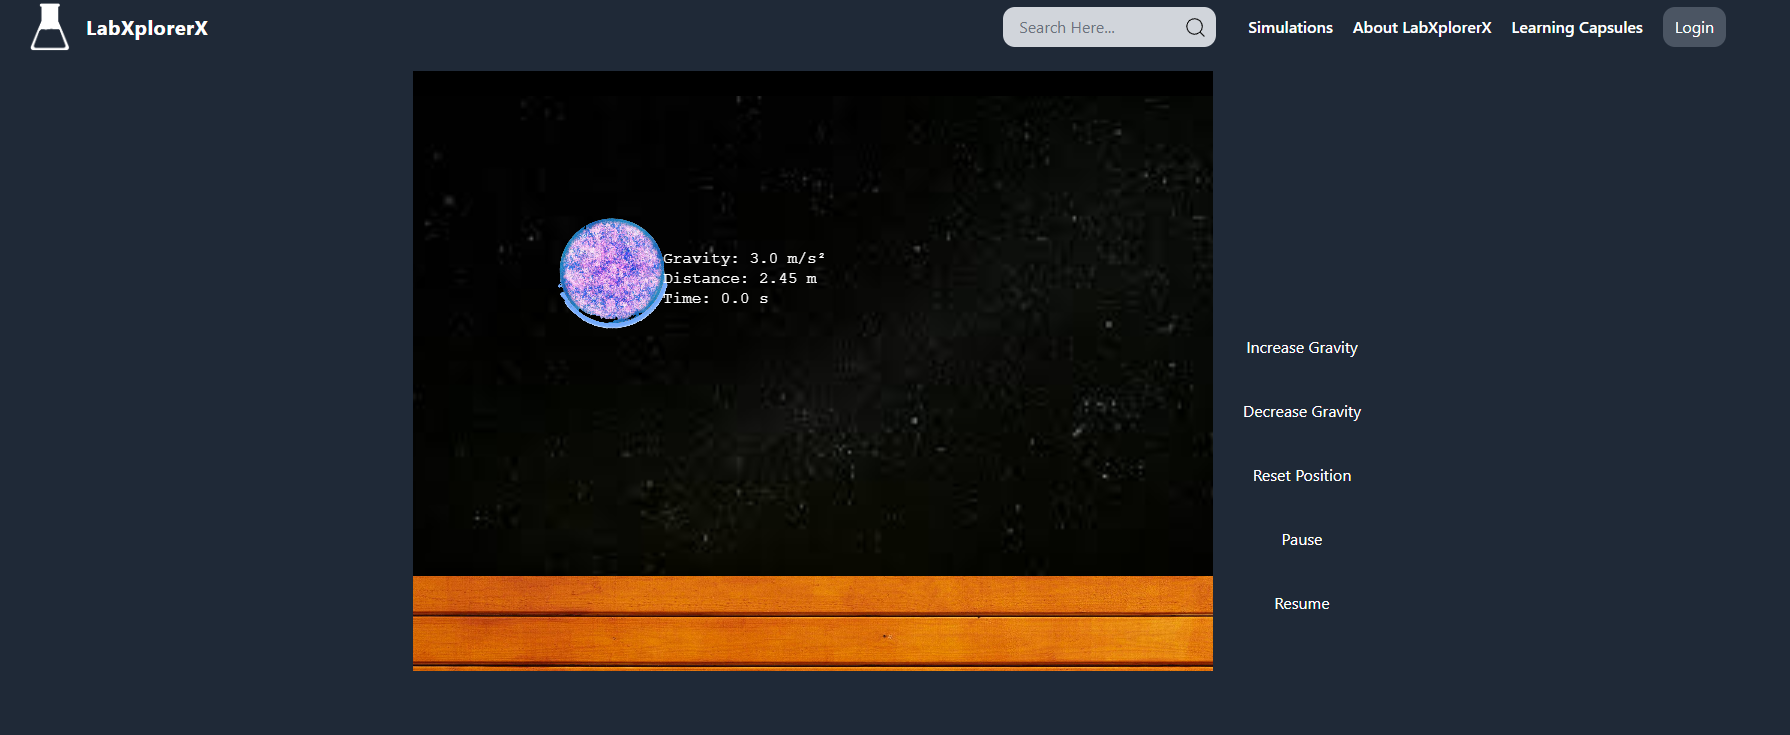
\includegraphics[width = 16cm]{Diagrams/output/gravity.png}
     \caption{Gravity Simulator}
 \end{figure}

 \begin{figure}[H]
    \centering
     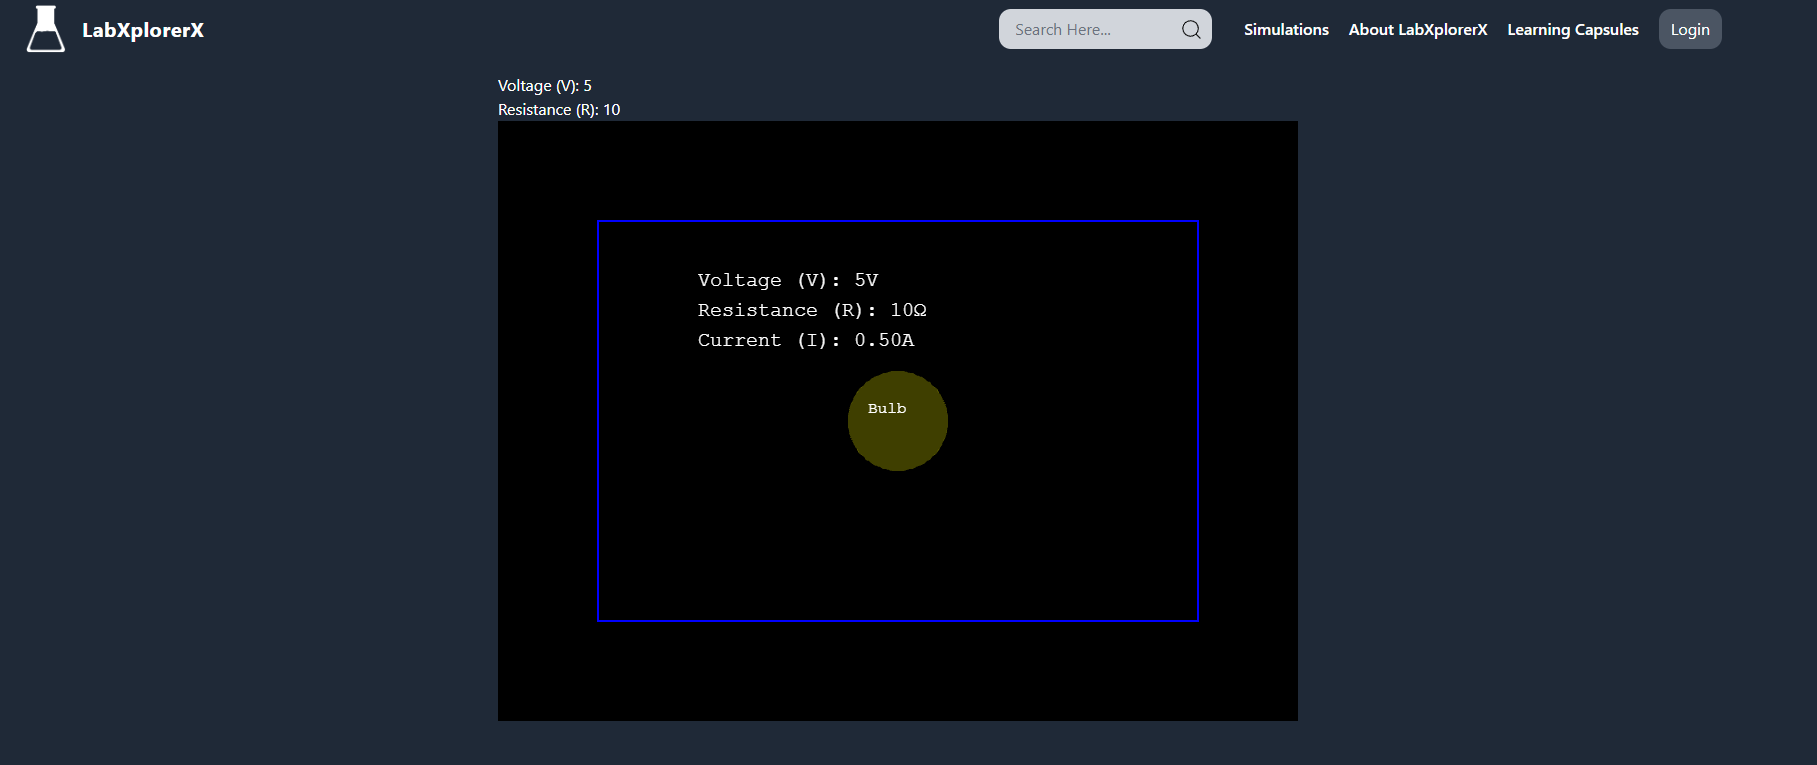
\includegraphics[width = 16cm]{Diagrams/output/ohms.png}
     \caption{Ohms Law Simulator}
 \end{figure}

 \begin{figure}[H]
    \centering
     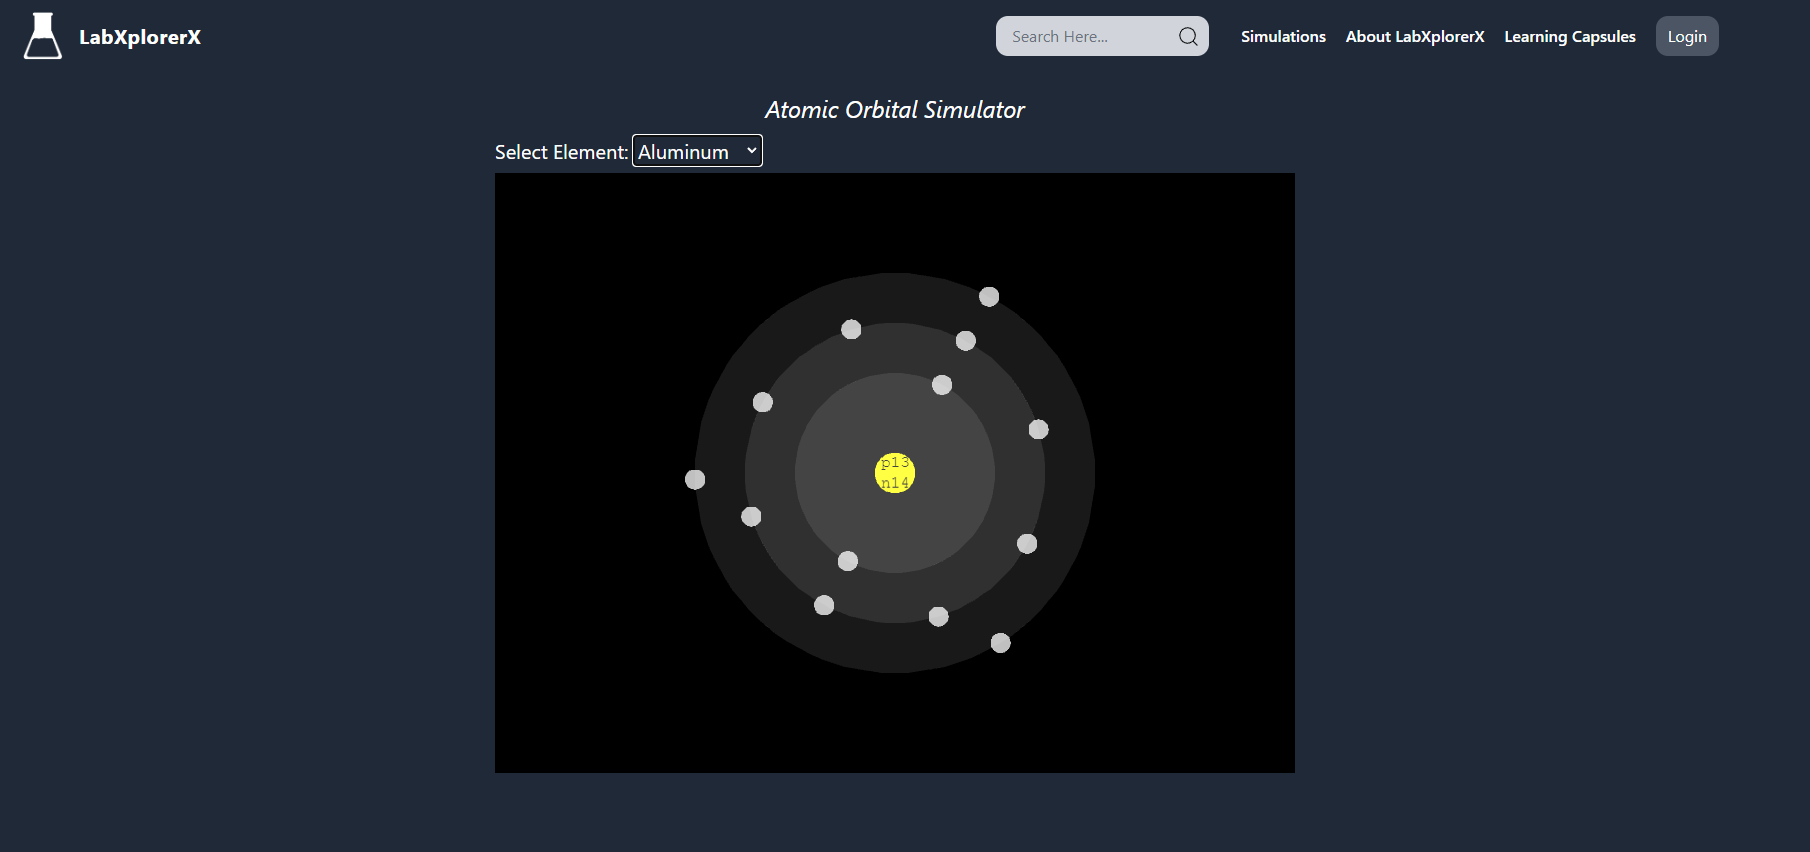
\includegraphics[width = 16cm]{Diagrams/output/atom.png}
     \caption{Atom Simulator}
 \end{figure}

 \begin{figure}[H]
    \centering
     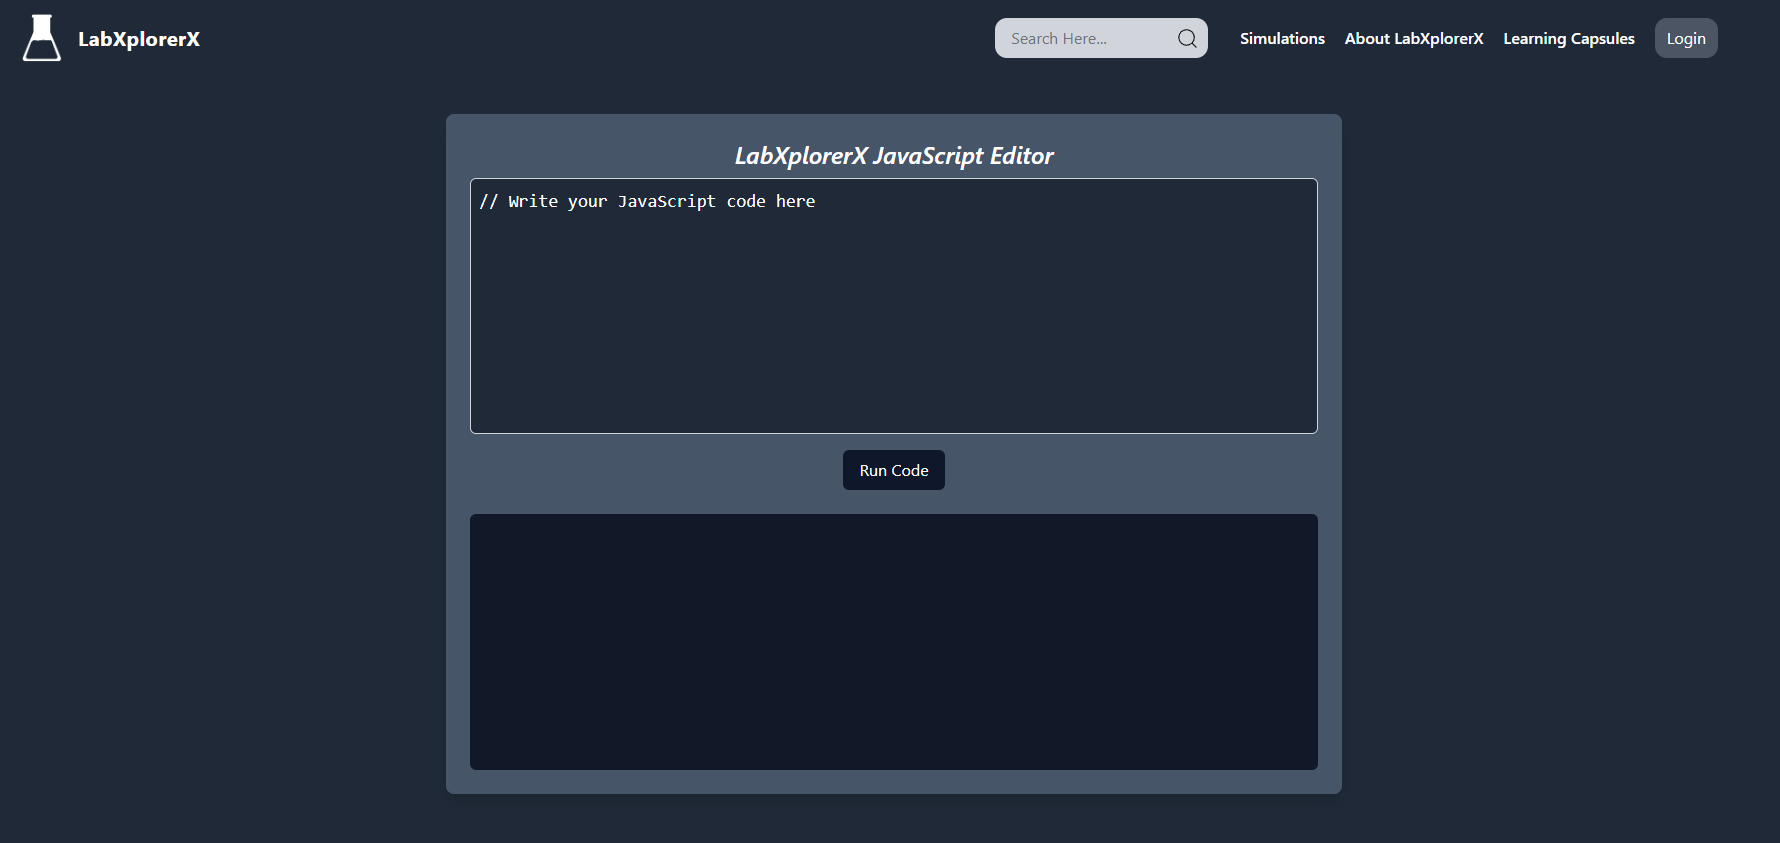
\includegraphics[width = 16cm]{Diagrams/output/js.png}
     \caption{JavaScript Editor}
 \end{figure}
 \begin{figure}[H]
    \centering
     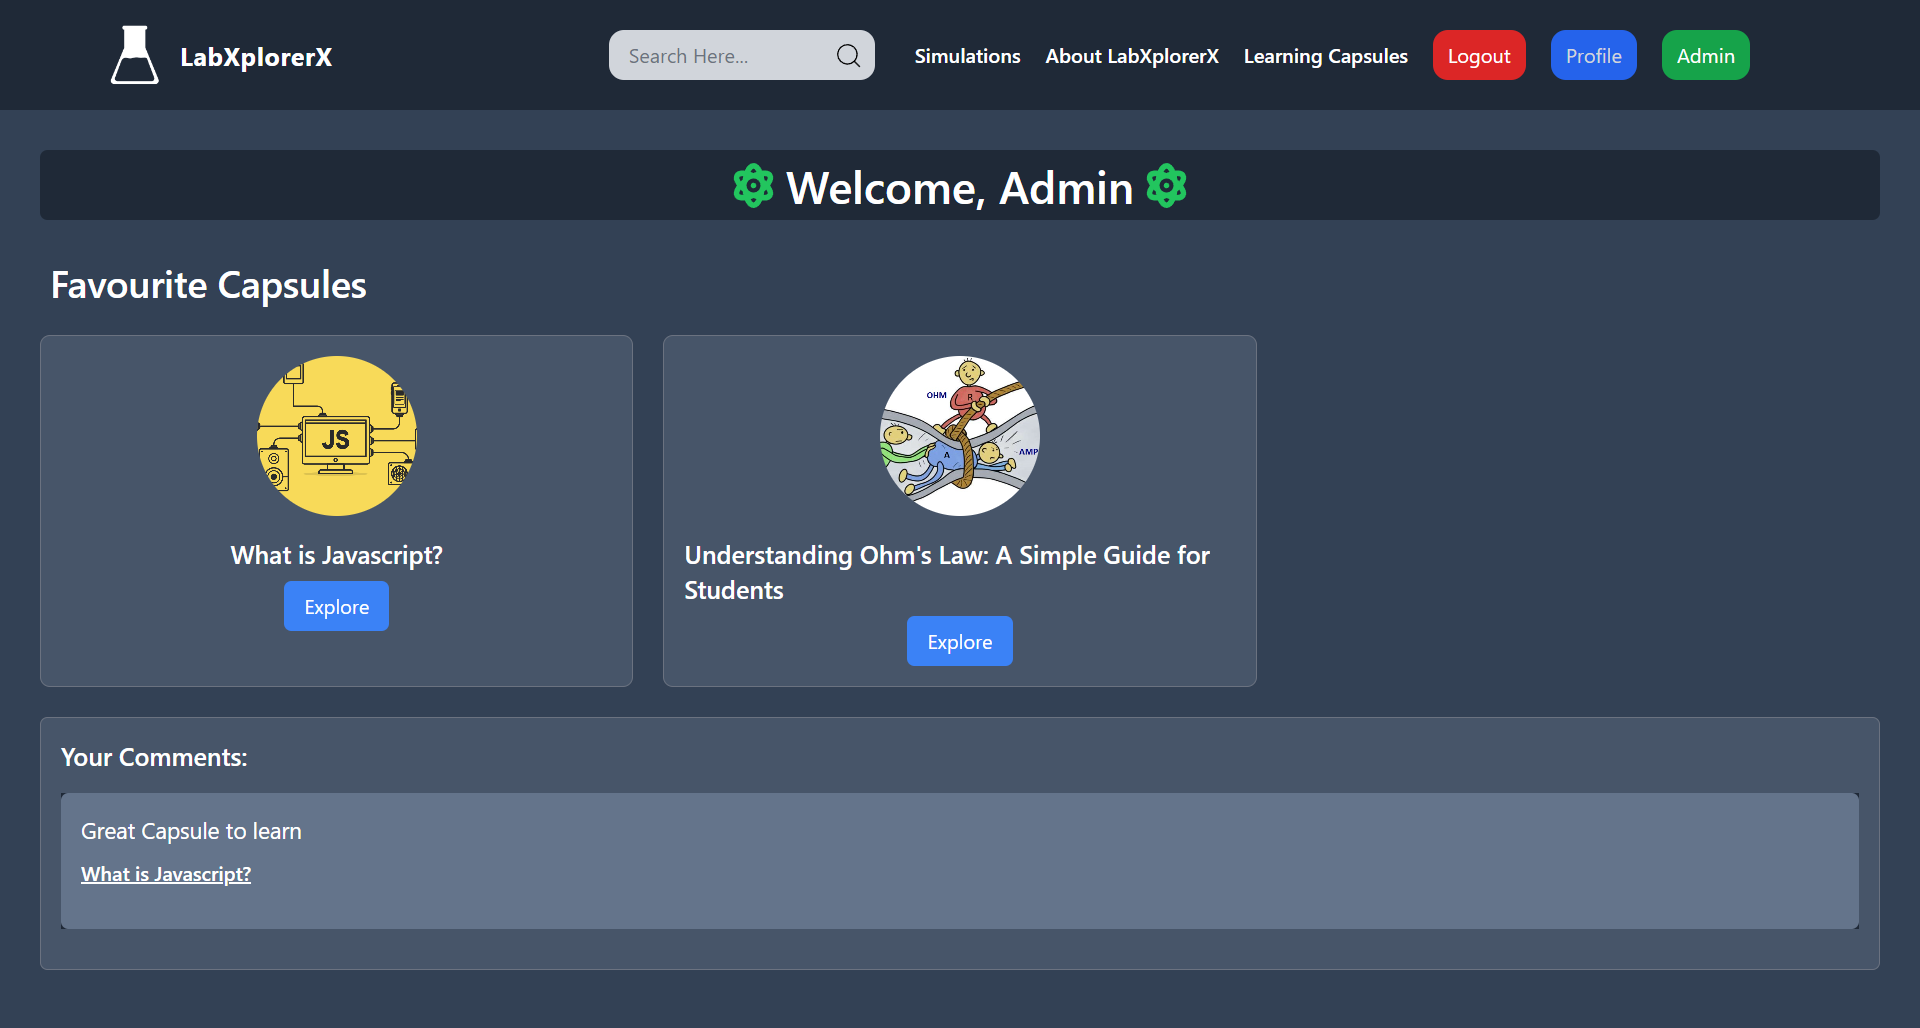
\includegraphics[width = 16cm]{Diagrams/output/profile.png}
     \caption{Profile}
 \end{figure}
 \begin{figure}[H]
    \centering
     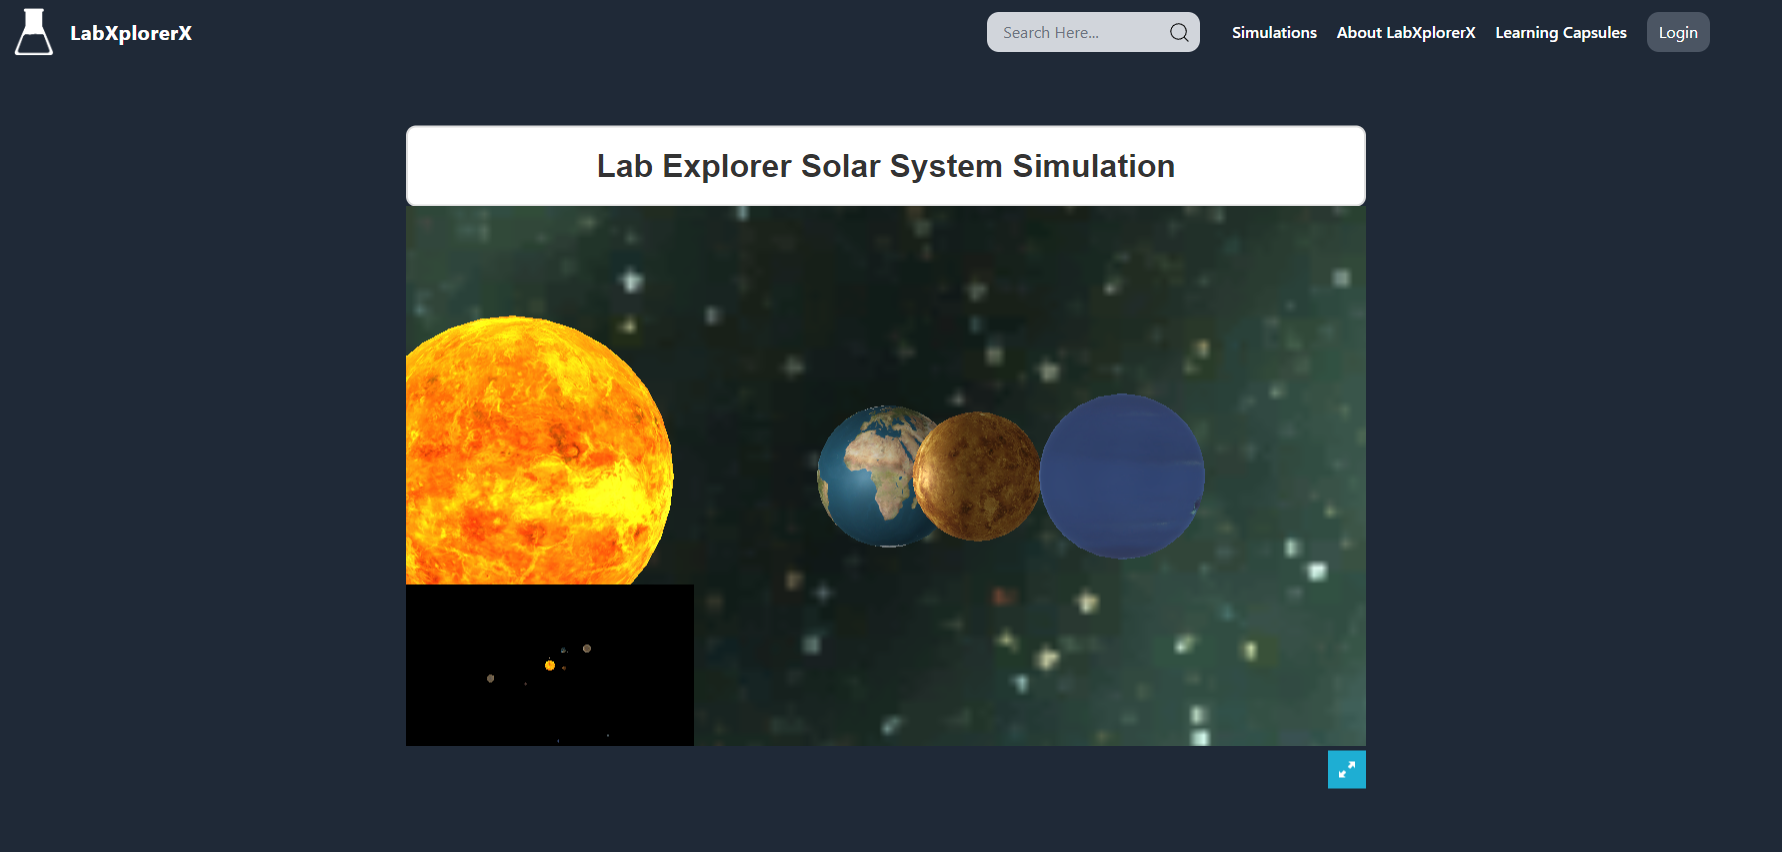
\includegraphics[width = 16cm]{Diagrams/output/solar.png}
     \caption{Solar System Simulator}
 \end{figure}
 \begin{figure}[H]
    \centering
     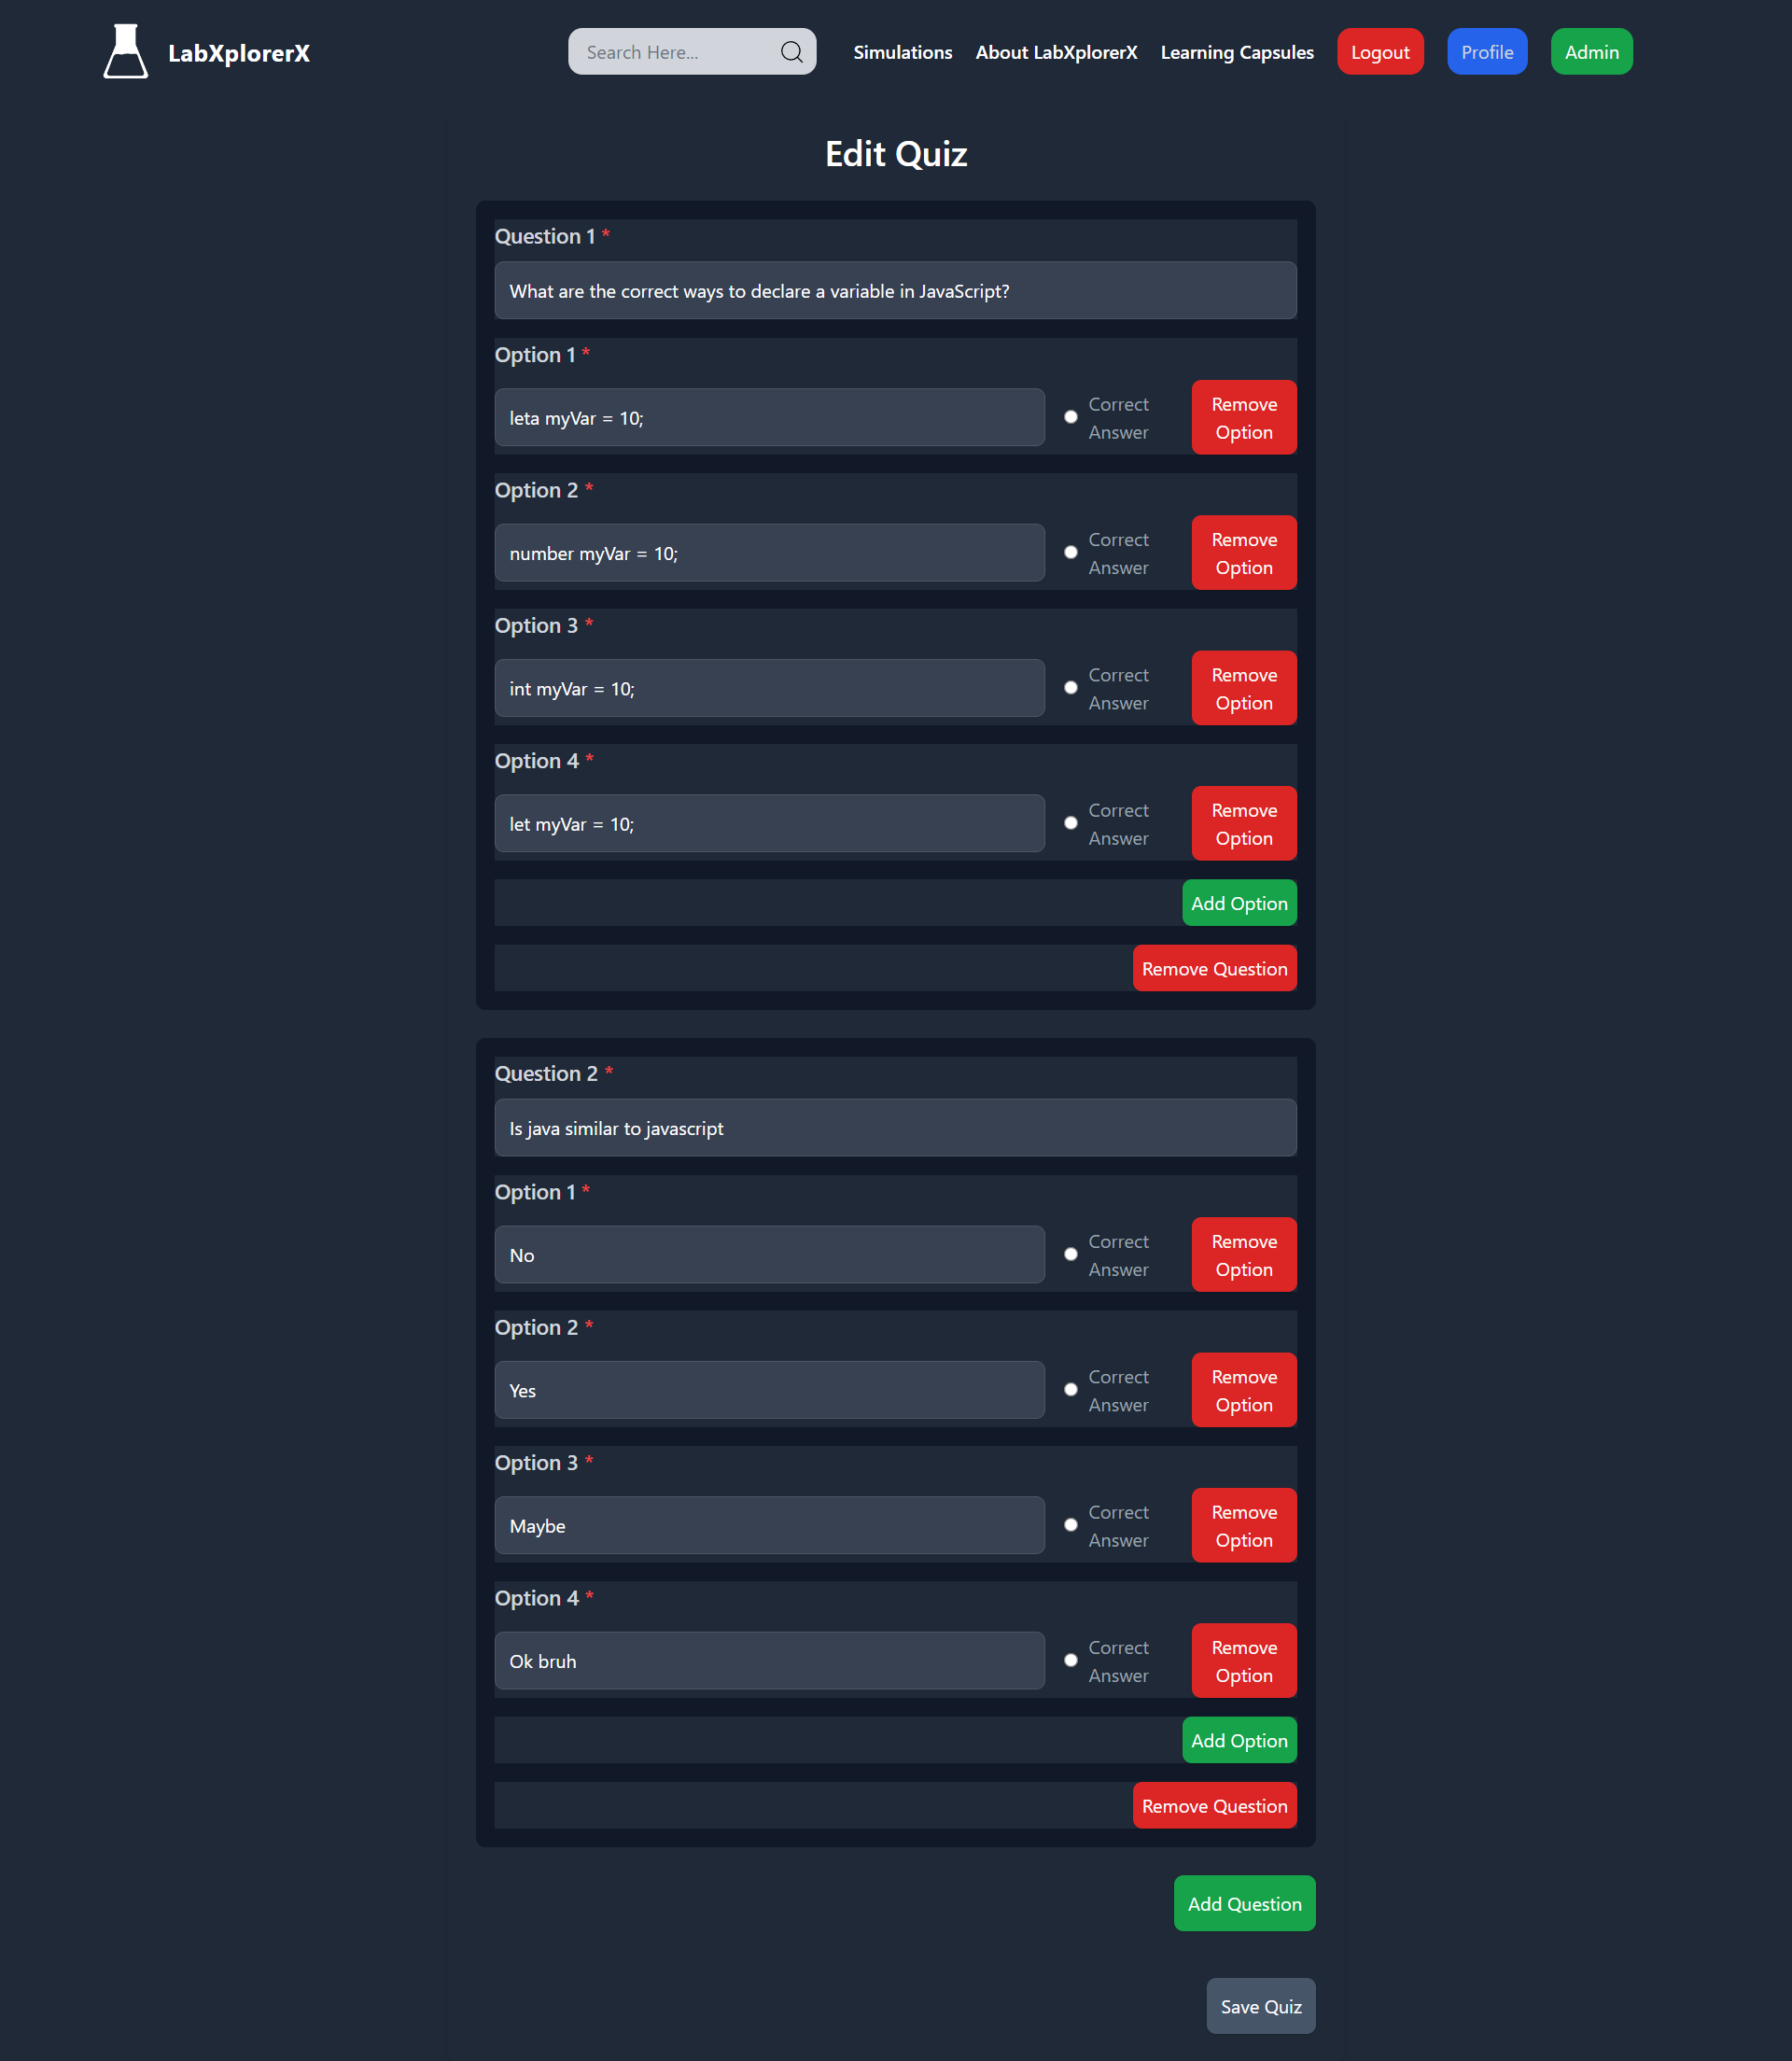
\includegraphics[width = 16cm]{Diagrams/output/edit_quiz.png}
     \caption{CRUD Quizes}
 \end{figure}
 \begin{figure}[H]
    \centering
     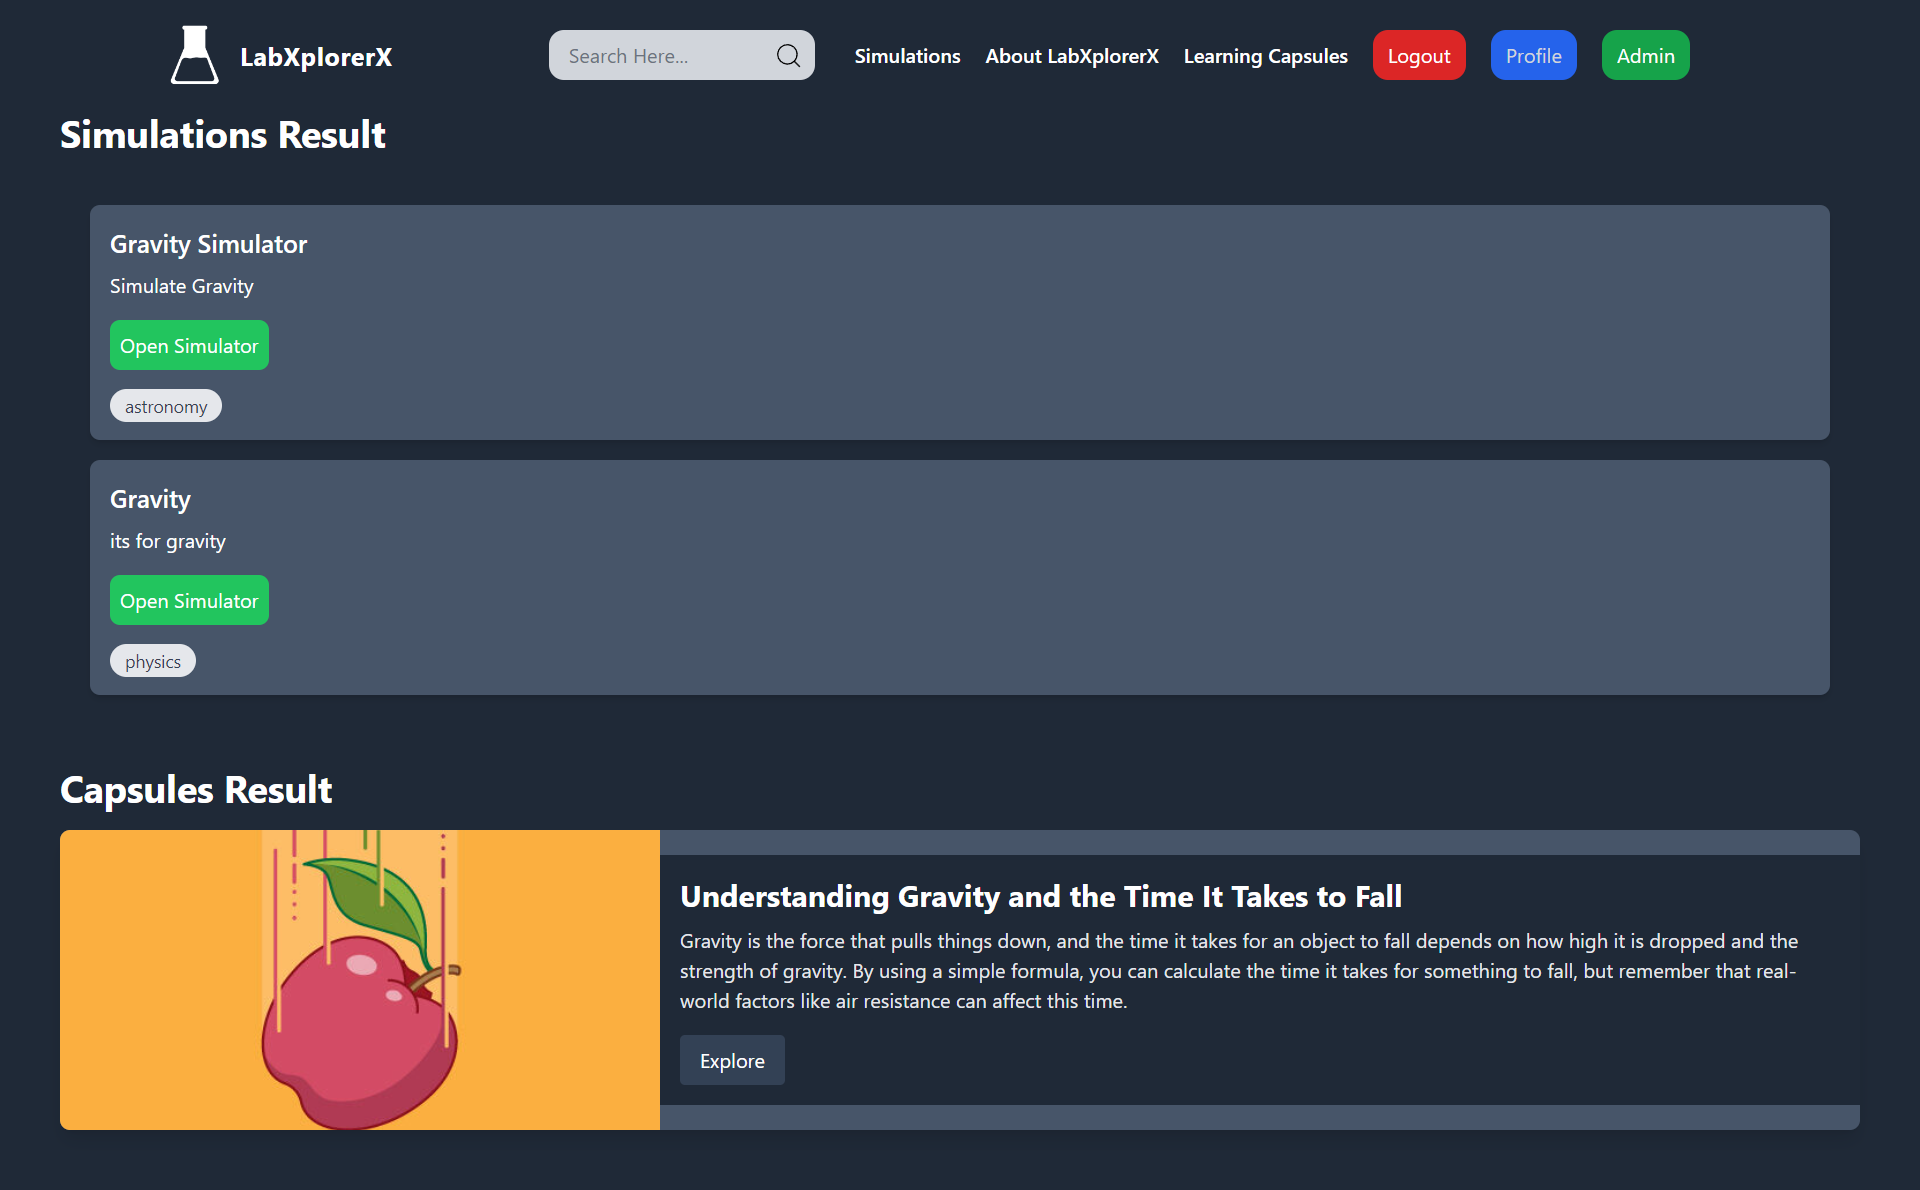
\includegraphics[width = 16cm]{Diagrams/output/search_results.png}
     \caption{Search Results}
 \end{figure}
 \begin{figure}[H]
    \centering
     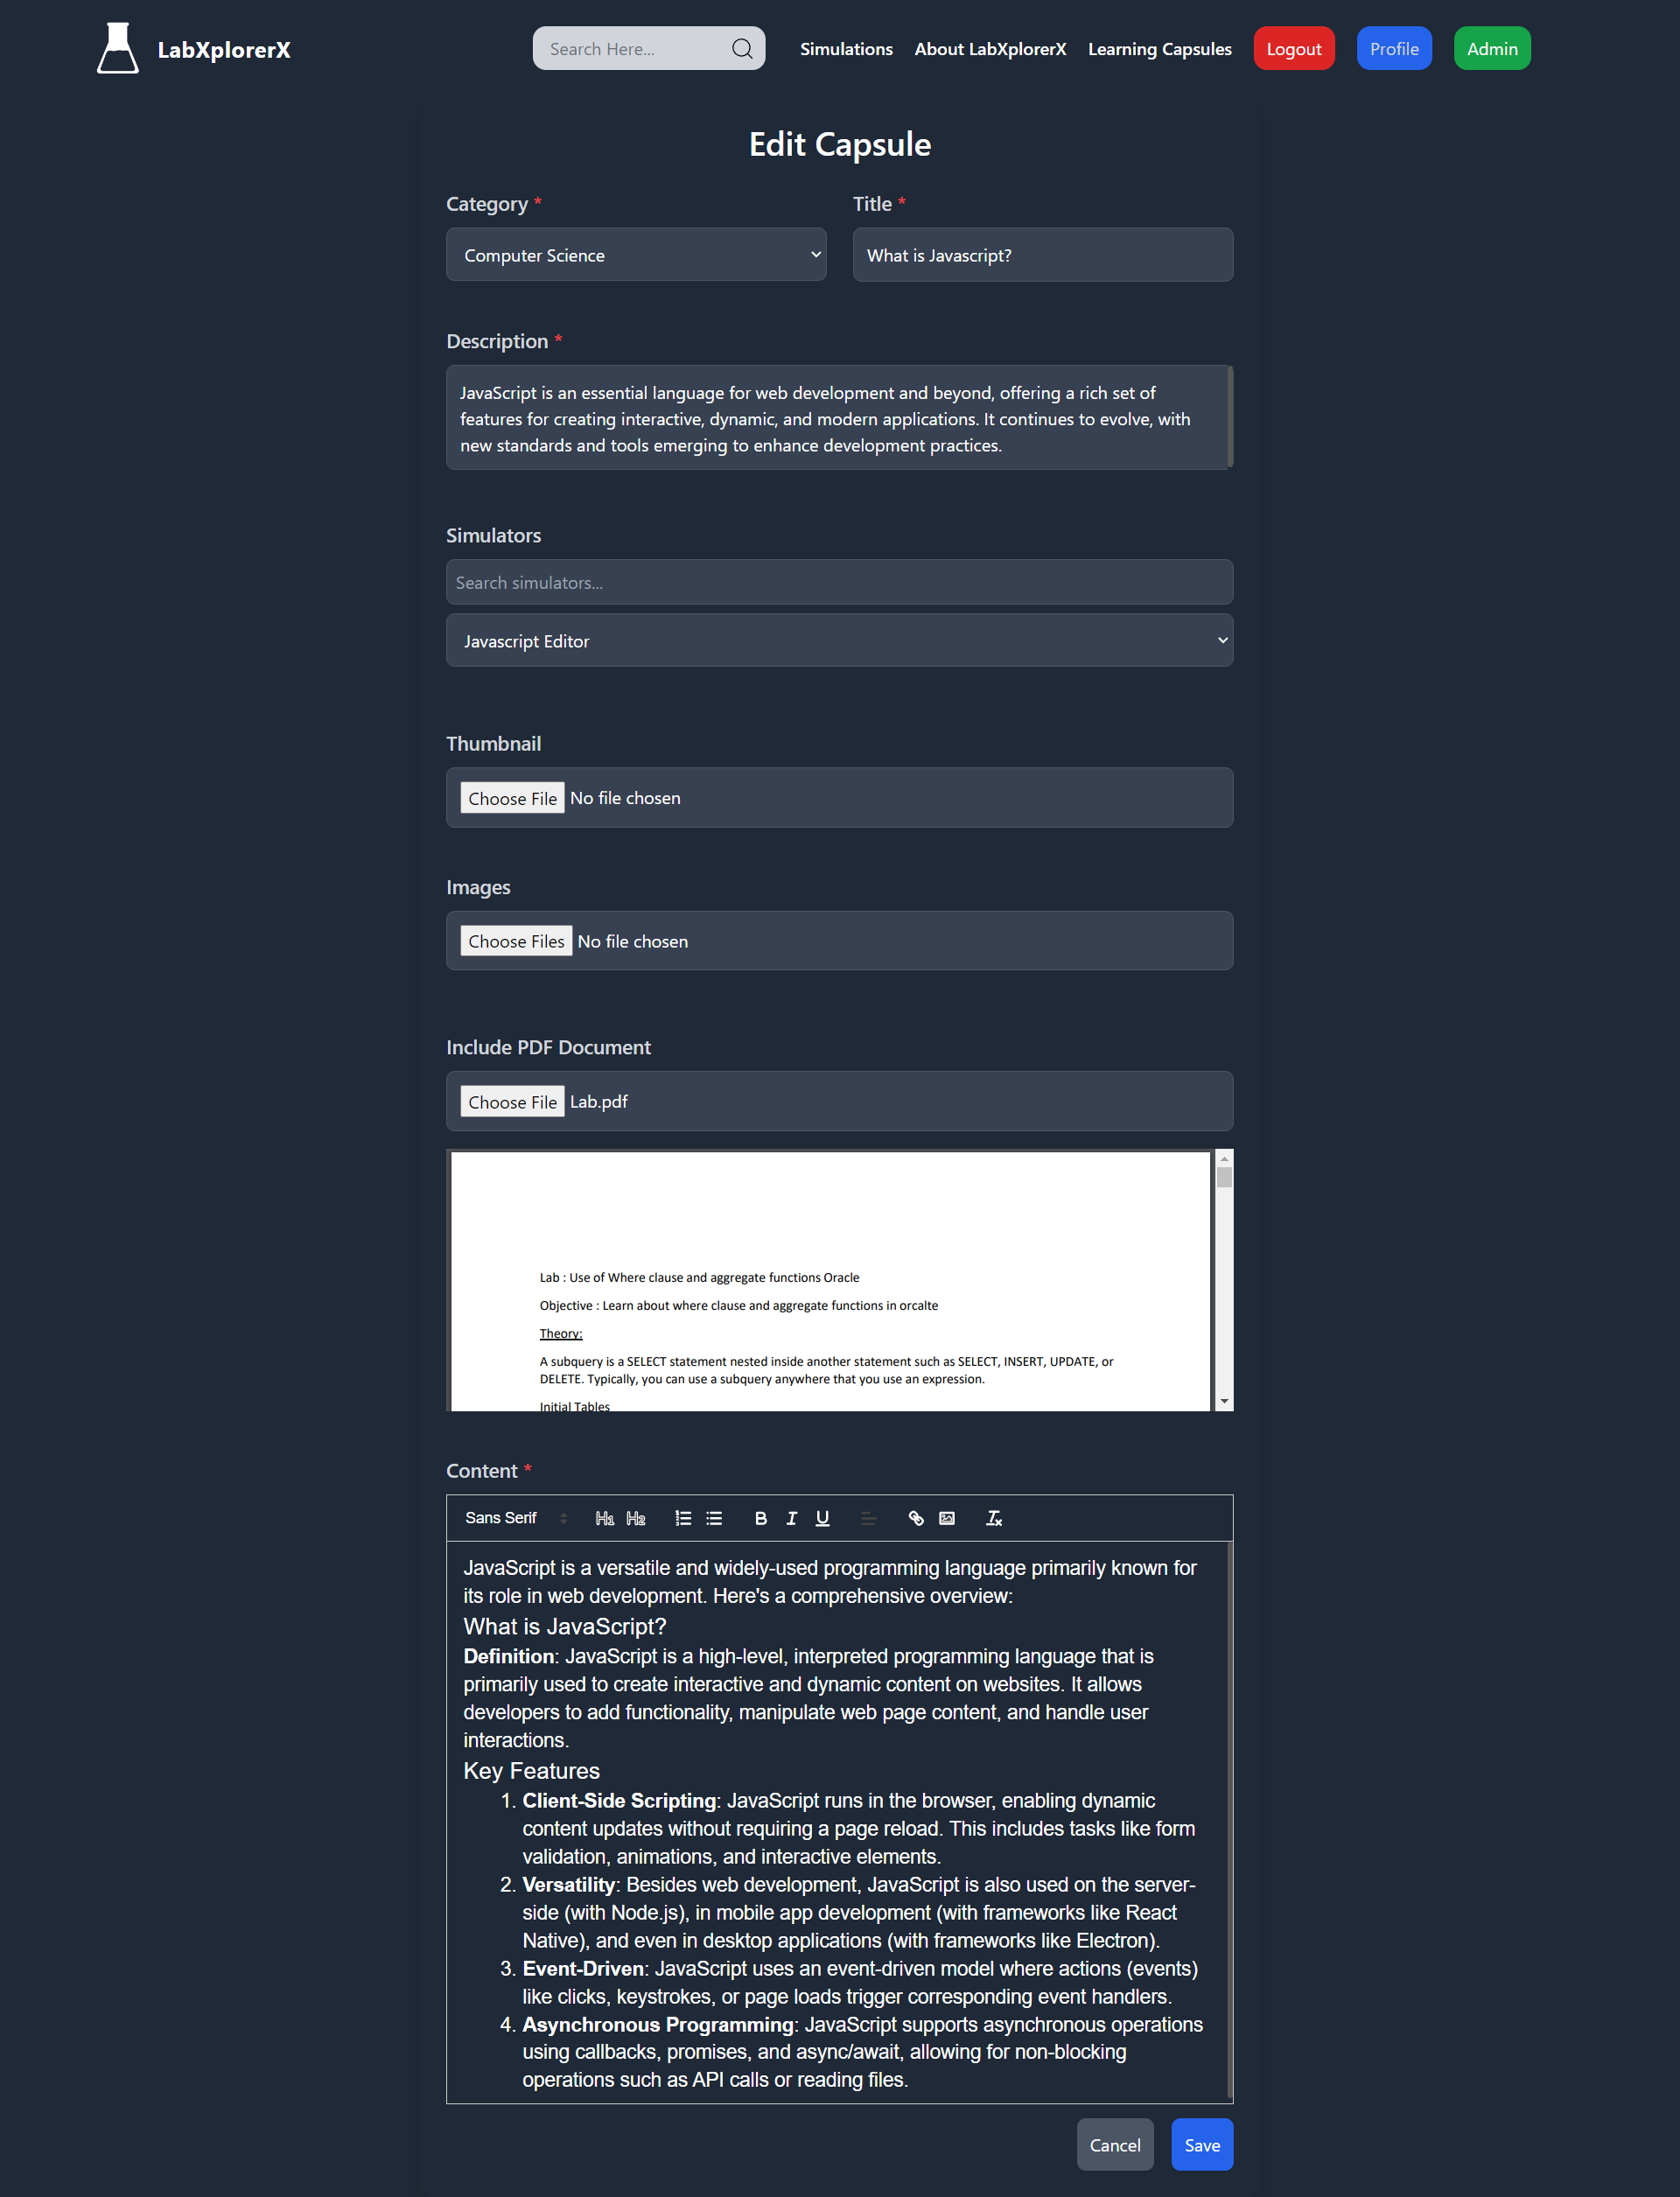
\includegraphics[width = 16cm]{Diagrams/output/edit_capsule.png}
     \caption{Edit Capsule}
 \end{figure}
 \begin{figure}[H]
    \centering
     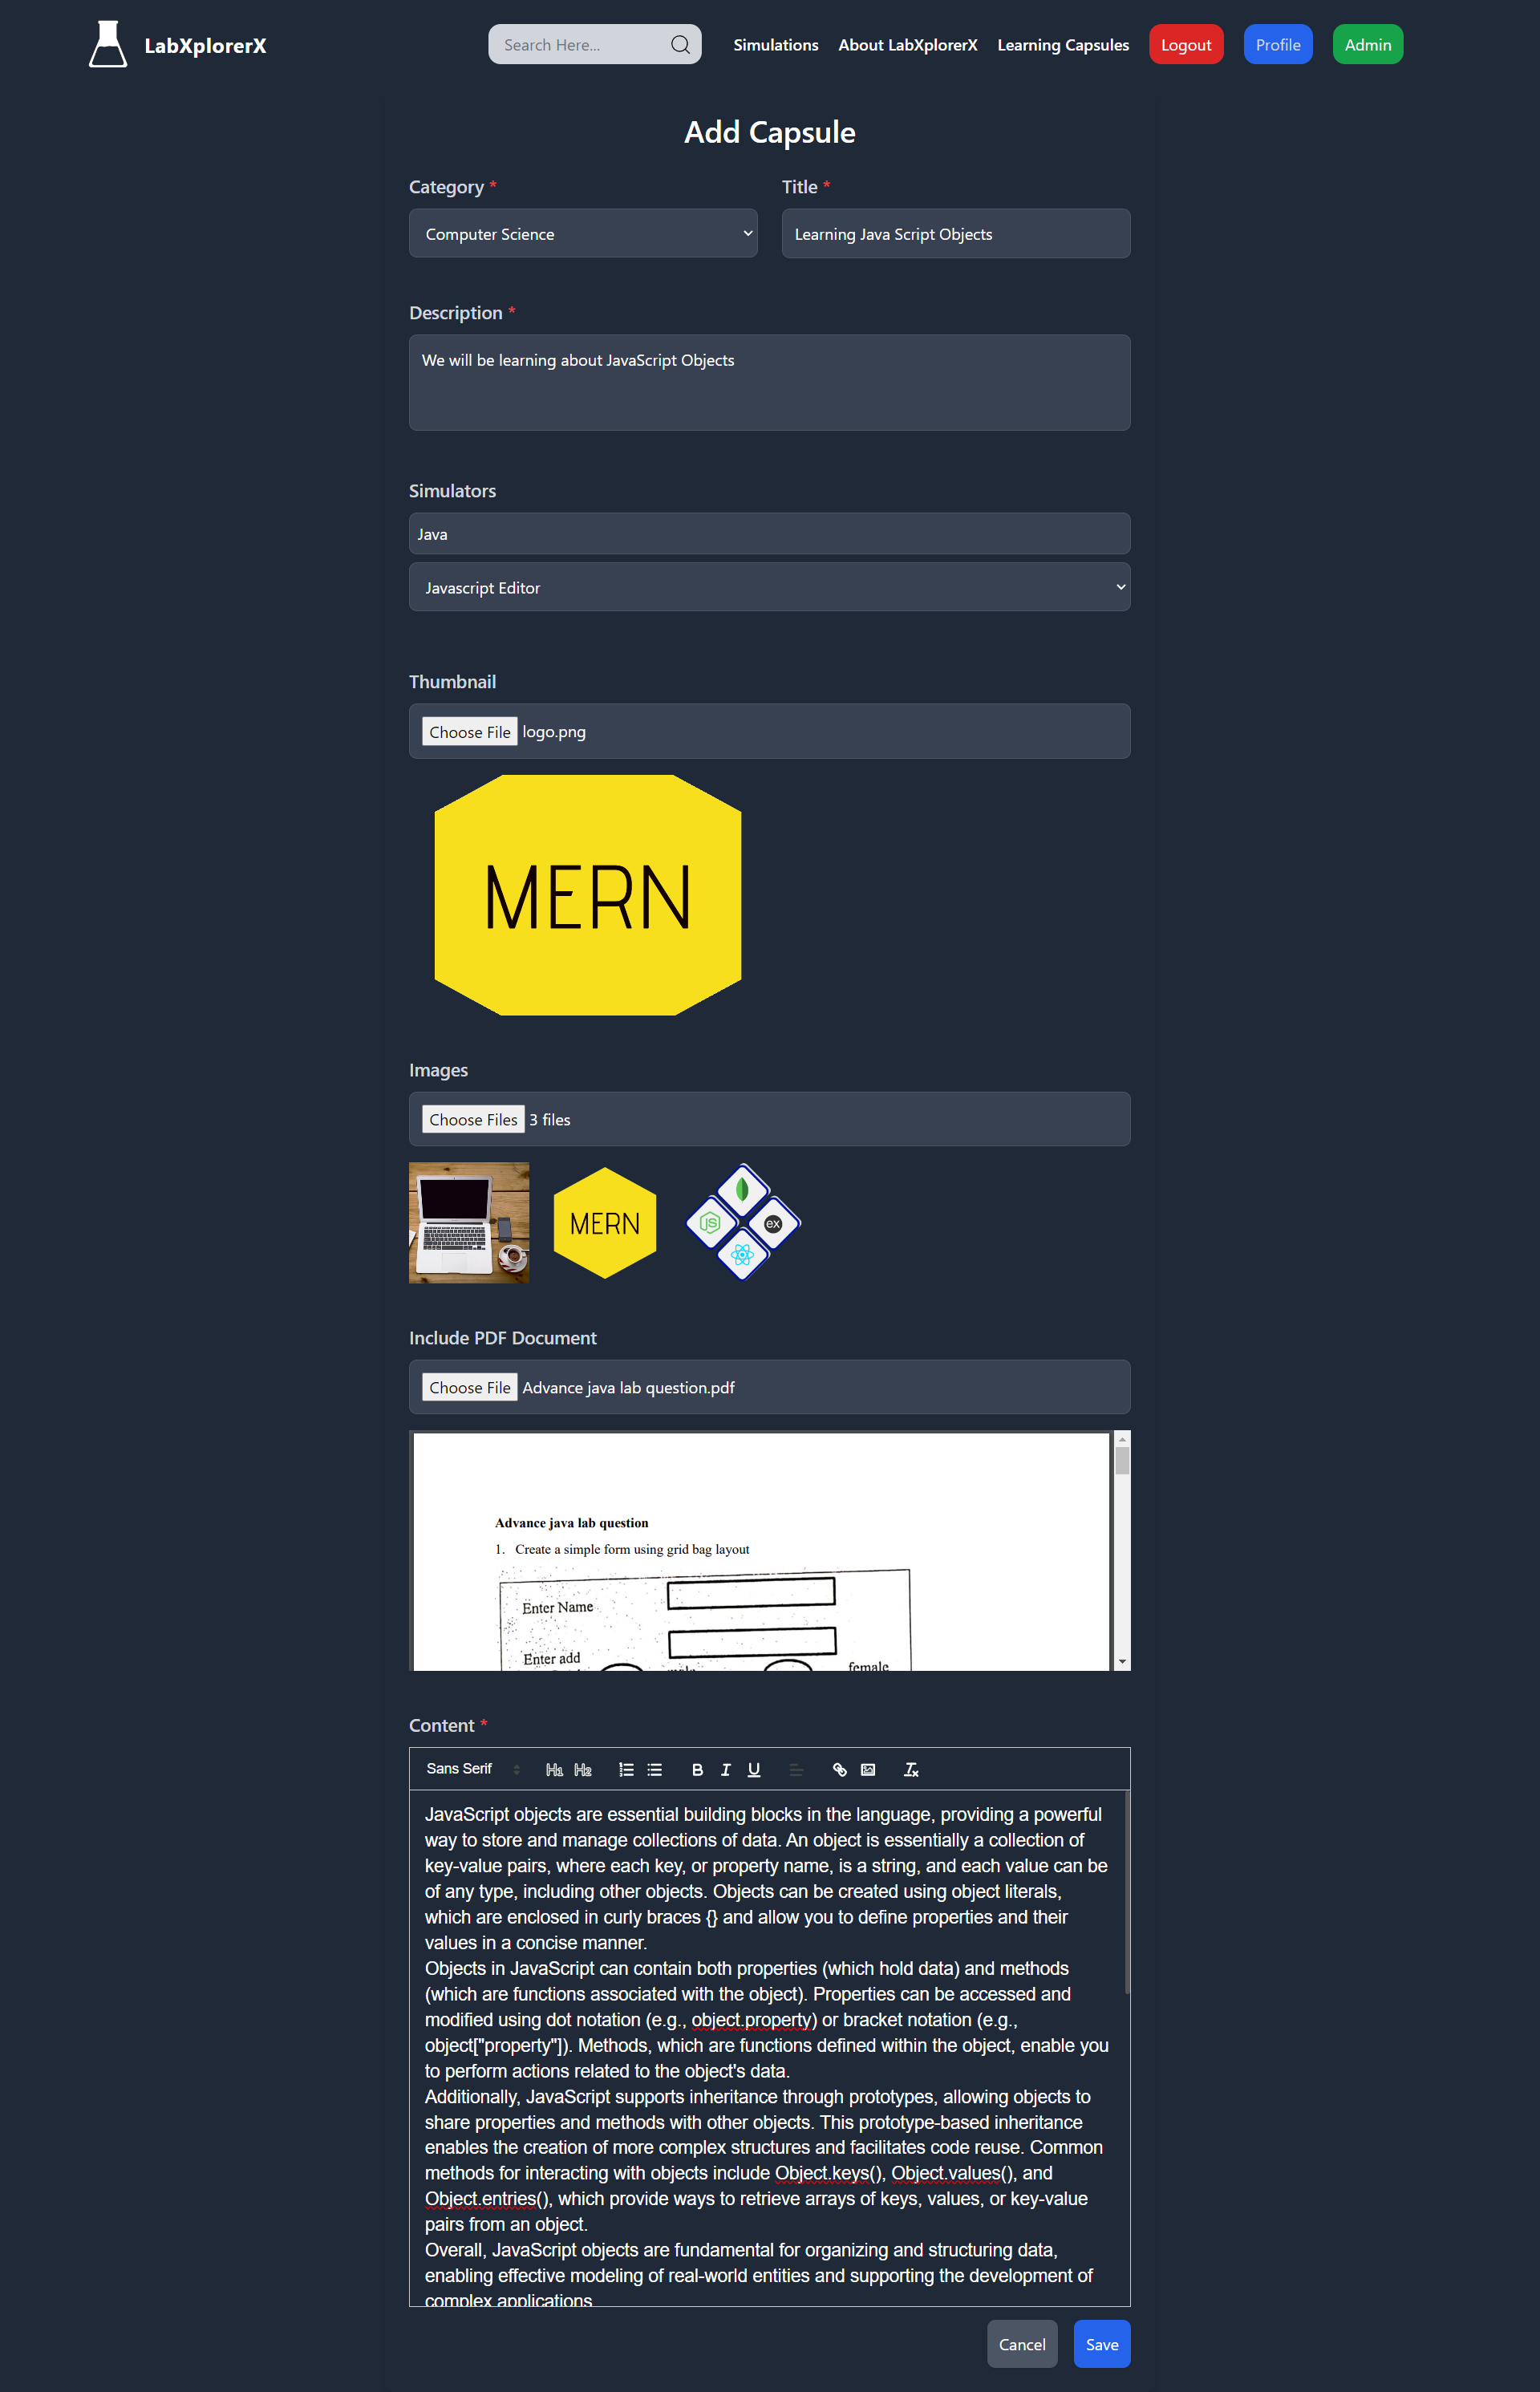
\includegraphics[width = 15cm]{Diagrams/output/addcapsule.png}
     \caption{Add Capsule}
 \end{figure}
 \begin{figure}[H]
    \centering
     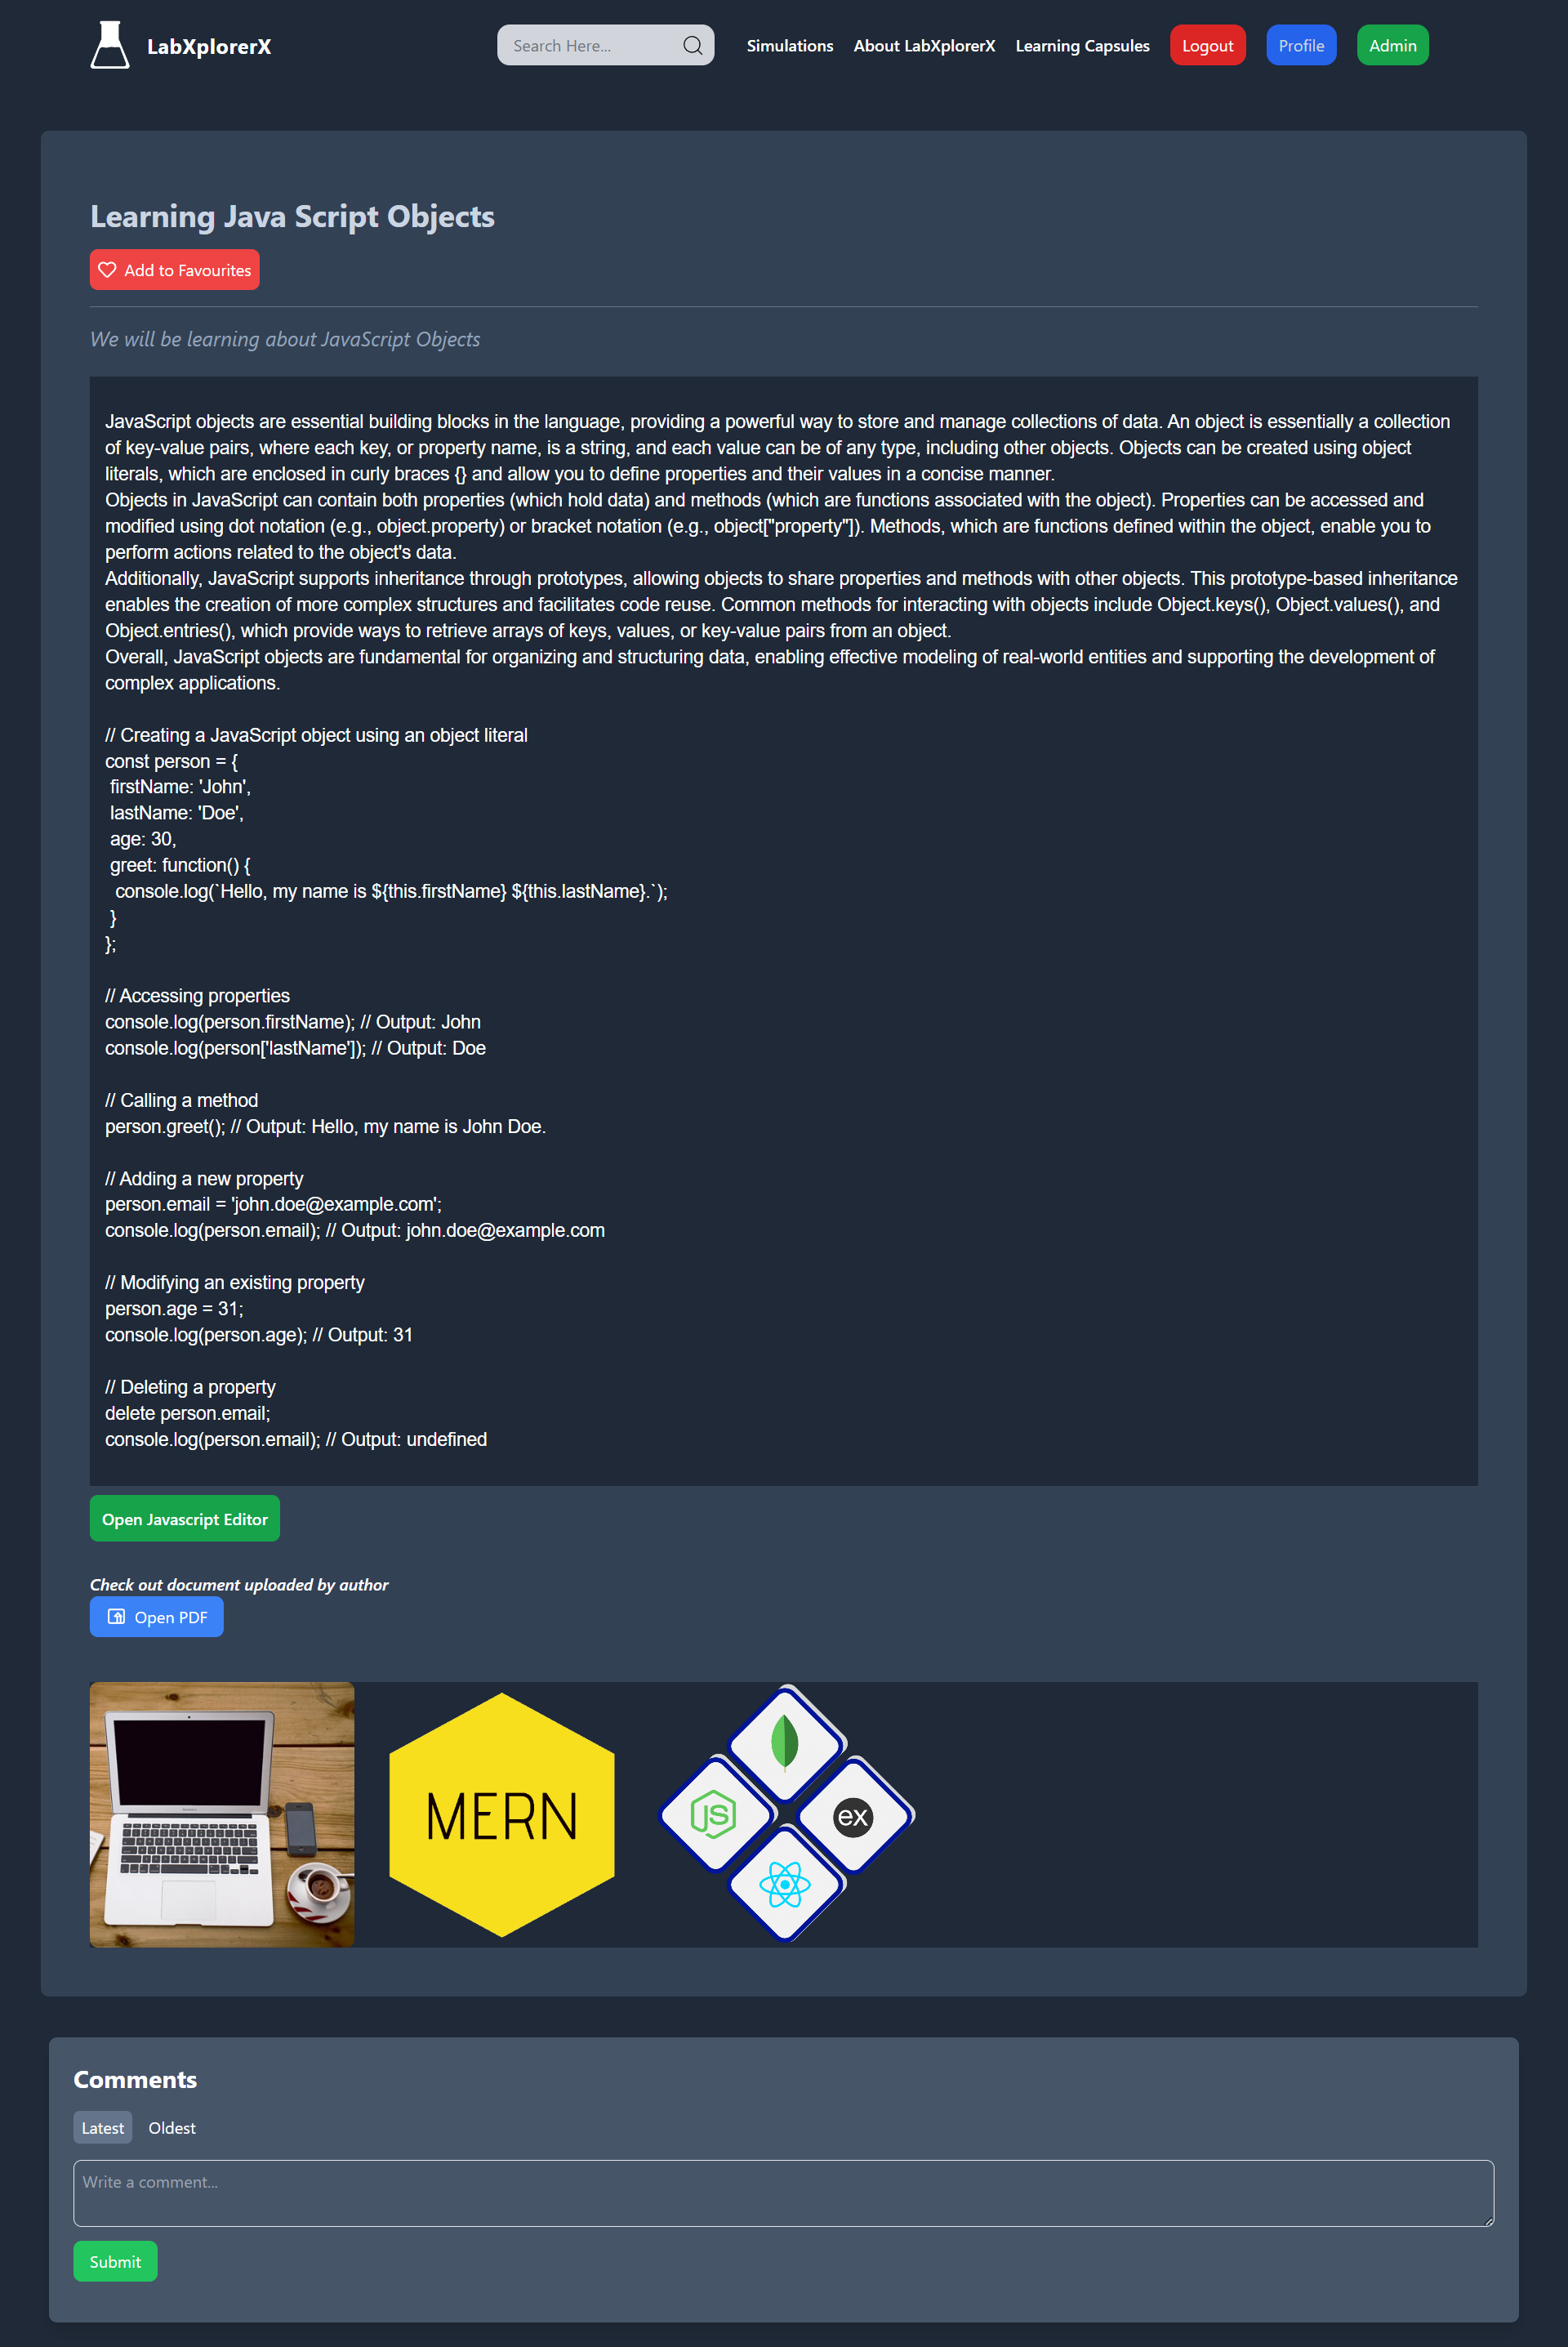
\includegraphics[width = 16cm]{Diagrams/output/after_addition.png}
     \caption{After Additon of Capsule}
 \end{figure}
\section{Work Remaining}
As the LabXplorerX project progresses, several key tasks remain to be completed. The development team will focus on creating additional simulations to further expand the interactive learning opportunities available to students. The implementation of user profiles is also pending, which will enable students to personalize their learning experience, track progress, and manage their accounts. Additionally, a discussion forum needs to be integrated into the platform, allowing students and teachers to engage in meaningful conversations, share ideas, and collaborate on learning activities.

\begin{itemize}[leftmargin=1cm]
    \item \textbf{More Simulations:} Continue creating additional simulations to broaden the range of interactive learning experiences available to students.
    
    \item \textbf{User Profiles:} Implement personalized user profiles, enabling students to track their progress, manage their accounts, and enhance their learning experience.
    
    \item \textbf{Discussion Forum:} Develop and integrate a discussion forum, facilitating communication and collaboration between students and teachers within the platform.
\end{itemize}

% ================================Appendices Setup================================================


\begin{appendices}
\renewcommand\thechapter{A}
\renewcommand\thefigure{\thechapter.\arabic{figure}}
\chapter*{APPENDIX A}
\addtocontents{toc}{\textbf{APPENDIX A}}
\section{Project Schedule}
Below is the Gantt chart for the project schedule. Specific tasks are planned to be performed within the designated time frames as illustrated. This chart provides a visual representation of the project's timeline, highlighting the start and end dates for each task, as well as their dependencies. By following this schedule, the project team can effectively manage resources, track progress, and ensure timely completion of each phase.
\begin{figure}[H]
    \centering
        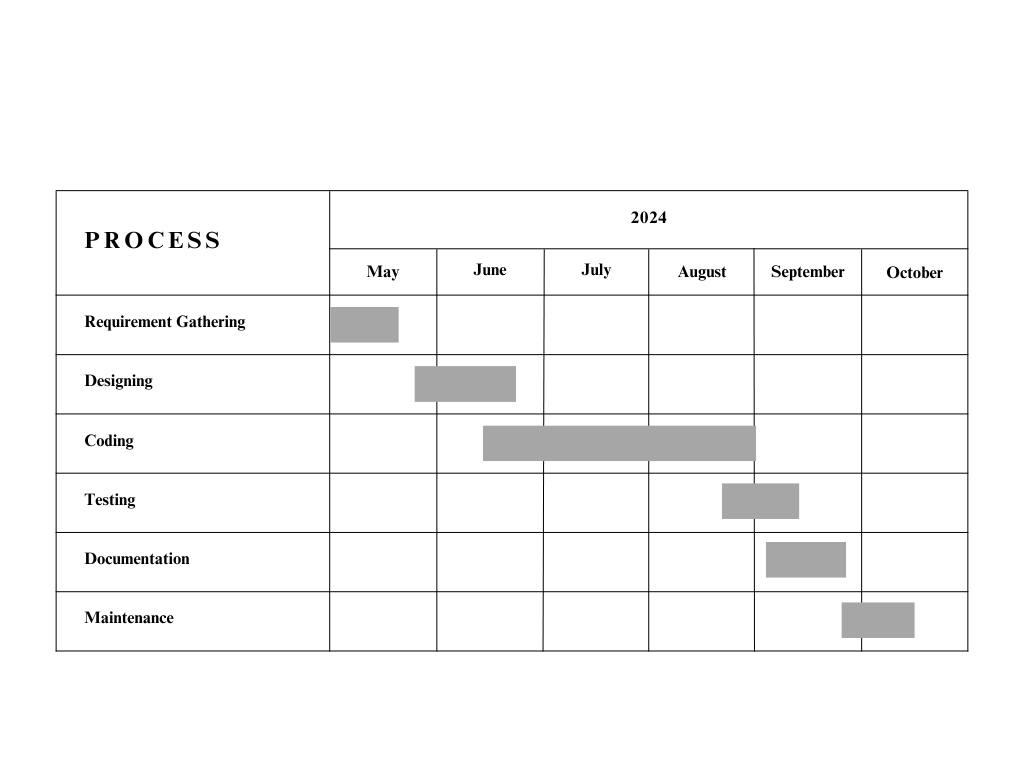
\includegraphics[width=400px]{Diagrams/Gantt_Chart.png}
    \caption{Gantt Chart of Schedule}
\end{figure}
\section{Running the Project}

\begin{itemize}
    \item \textbf{Cloning the Repository}
    \begin{enumerate}[label=\textbf{Step \arabic*:}]
        \item \textbf{Open a Terminal or Command Prompt.}
        \item \textbf{Navigate to the Directory Where You Want to Clone the Repository.}
        \begin{verbatim}
        cd path/to/your/directory
        \end{verbatim}
        \item \textbf{Clone the Repository.}
        \begin{verbatim}
        git clone https://github.com/sushantbramhacharya/
        LabXplorer_Proj.git
        \end{verbatim}
        \item \textbf{Navigate into the Cloned Repository.}
        \begin{verbatim}
        cd LabXplorer_Proj
        \end{verbatim}
    \end{enumerate}
    
    \item \textbf{Restoring the SQL File in pgAdmin}
    \begin{enumerate}[label=\textbf{Step \arabic*:}]
        \item \textbf{Open pgAdmin.}
        \item \textbf{Connect to Your PostgreSQL Server.}
        \begin{itemize}
            \item If you haven’t already set up a server connection, add a new connection using your server credentials.
        \end{itemize}
        \item \textbf{Create a New Database (If Needed).}
        \begin{itemize}
            \item Right-click on the “Databases” node and select “Create > Database...”
            \item Enter a name for your database and click “Save.”
        \end{itemize}
        \item \textbf{Restore the Database from the SQL File.}
        \begin{itemize}
            \item Right-click on your database and select “Restore.”
            \item In the “Restore” dialog, select the “File” tab.
            \item Click the “...” button to browse for the SQL file you want to restore.
            \item Select the SQL file and click “Restore.”
        \end{itemize}
        \item \textbf{Verify the Restoration.}
        \begin{itemize}
            \item Expand the “Schemas” and “Tables” nodes to ensure that your database schema and tables have been correctly restored.
        \end{itemize}
    \end{enumerate}
    
    \item \textbf{Running the Project}
    \begin{enumerate}[label=\textbf{Step \arabic*:}]
        \item \textbf{Ensure Node.js and npm Are Installed.}
        \begin{itemize}
            \item Check if Node.js and npm are installed by running:
            \begin{verbatim}
            node -v
            npm -v
            \end{verbatim}
            \item If not installed, download and install Node.js from \texttt{https://nodejs.org}.
        \end{itemize}
        \item \textbf{Install Project Dependencies.}
        \begin{verbatim}
        npm install
        \end{verbatim}
        \item \textbf{Start the Development Server.}
        \begin{verbatim}
        npm run dev
        \end{verbatim}
        \item \textbf{Access the Application.}
        \begin{itemize}
            \item Open your web browser and go to \texttt{http://localhost:5173} (or the port specified in your project configuration).
        \end{itemize}
    \end{enumerate}
\end{itemize}
\section{Basic Scene in Phaser.js}

Below is a simple example of creating a basic scene using Phaser.js. This scene displays a star image and some text, and logs the pointer coordinates when clicked.

\begin{lstlisting}[language=JavaScript,  basicstyle=\ttfamily, keywordstyle=\color{blue}, commentstyle=\color{green}]
const config = {
    type: Phaser.AUTO,
    width: 800,
    height: 600,
    backgroundColor: '#2d2d2d',
    scene: {
        preload: preload,
        create: create,
        update: update
    }
};
const game = new Phaser.Game(config);
function preload() {
    this.load.image('star', 'https://labs.phaser.io
/assets/sprites/star.png');
}
function create() {
    this.add.image(400, 300, 'star');
    this.add.text(10, 10, 'Hello Phaser!', 
    { font: '24px Arial', fill: '#ffffff' });
    this.input.on('pointerdown', function (pointer) {
        console.log('Pointer down at', pointer.x,
        pointer.y);
    });
}
function update() {
    // Game loop logic
}
\end{lstlisting}
\section{Postgres Database Tables}
\begin{figure}[H]
    \centering
        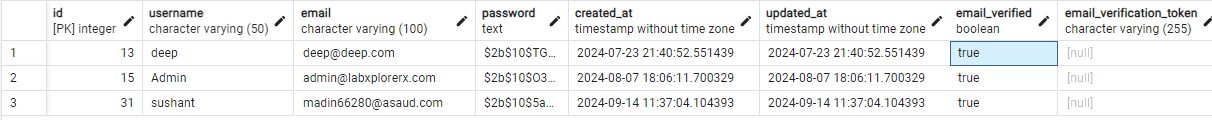
\includegraphics[width=430px]{Diagrams/db/user.png}
    \caption{Table of User}
\end{figure}
\begin{figure}[H]
    \centering
        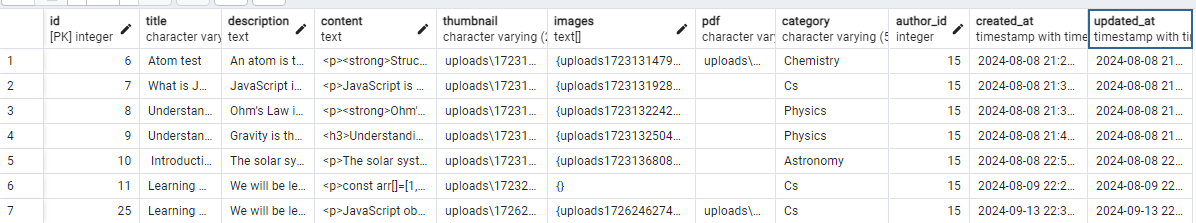
\includegraphics[width=430px]{Diagrams/db/capsules.png}
    \caption{Table of Capsule}
\end{figure}
\begin{figure}[H]
    \centering
        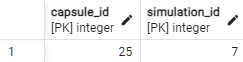
\includegraphics[width=120px]{Diagrams/db/capsule_sim.png}
    \caption{Table of Capsule Simulations}
\end{figure}
\begin{figure}[H]
    \centering
        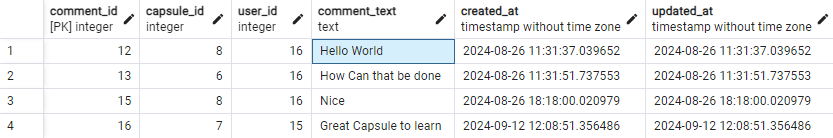
\includegraphics[width=430px]{Diagrams/db/comment.png}
    \caption{Table of Comments}
\end{figure}
\begin{figure}[H]
    \centering
        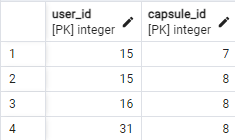
\includegraphics[width=120px]{Diagrams/db/fav.png}
    \caption{Table of Favourites}
\end{figure}
\begin{figure}[H]
    \centering
        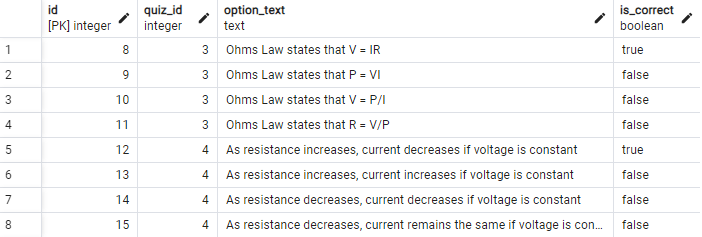
\includegraphics[width=400px]{Diagrams/db/options.png}
    \caption{Table of Quiz Options}
\end{figure}
\begin{figure}[H]
    \centering
        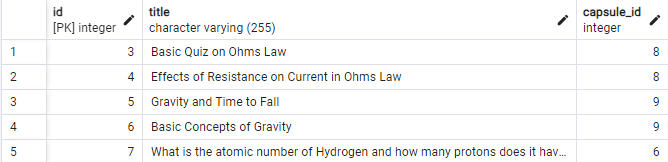
\includegraphics[width=400px]{Diagrams/db/quiz.png}
    \caption{Table of Quizes}
\end{figure}
\begin{figure}[H]
    \centering
        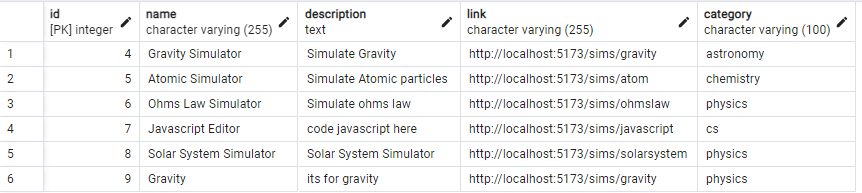
\includegraphics[width=430px]{Diagrams/db/sims.png}
    \caption{Table of Simulations}
\end{figure}
\section{Supervisor Consultation Form}
\begin{figure}[H]
    \centering
        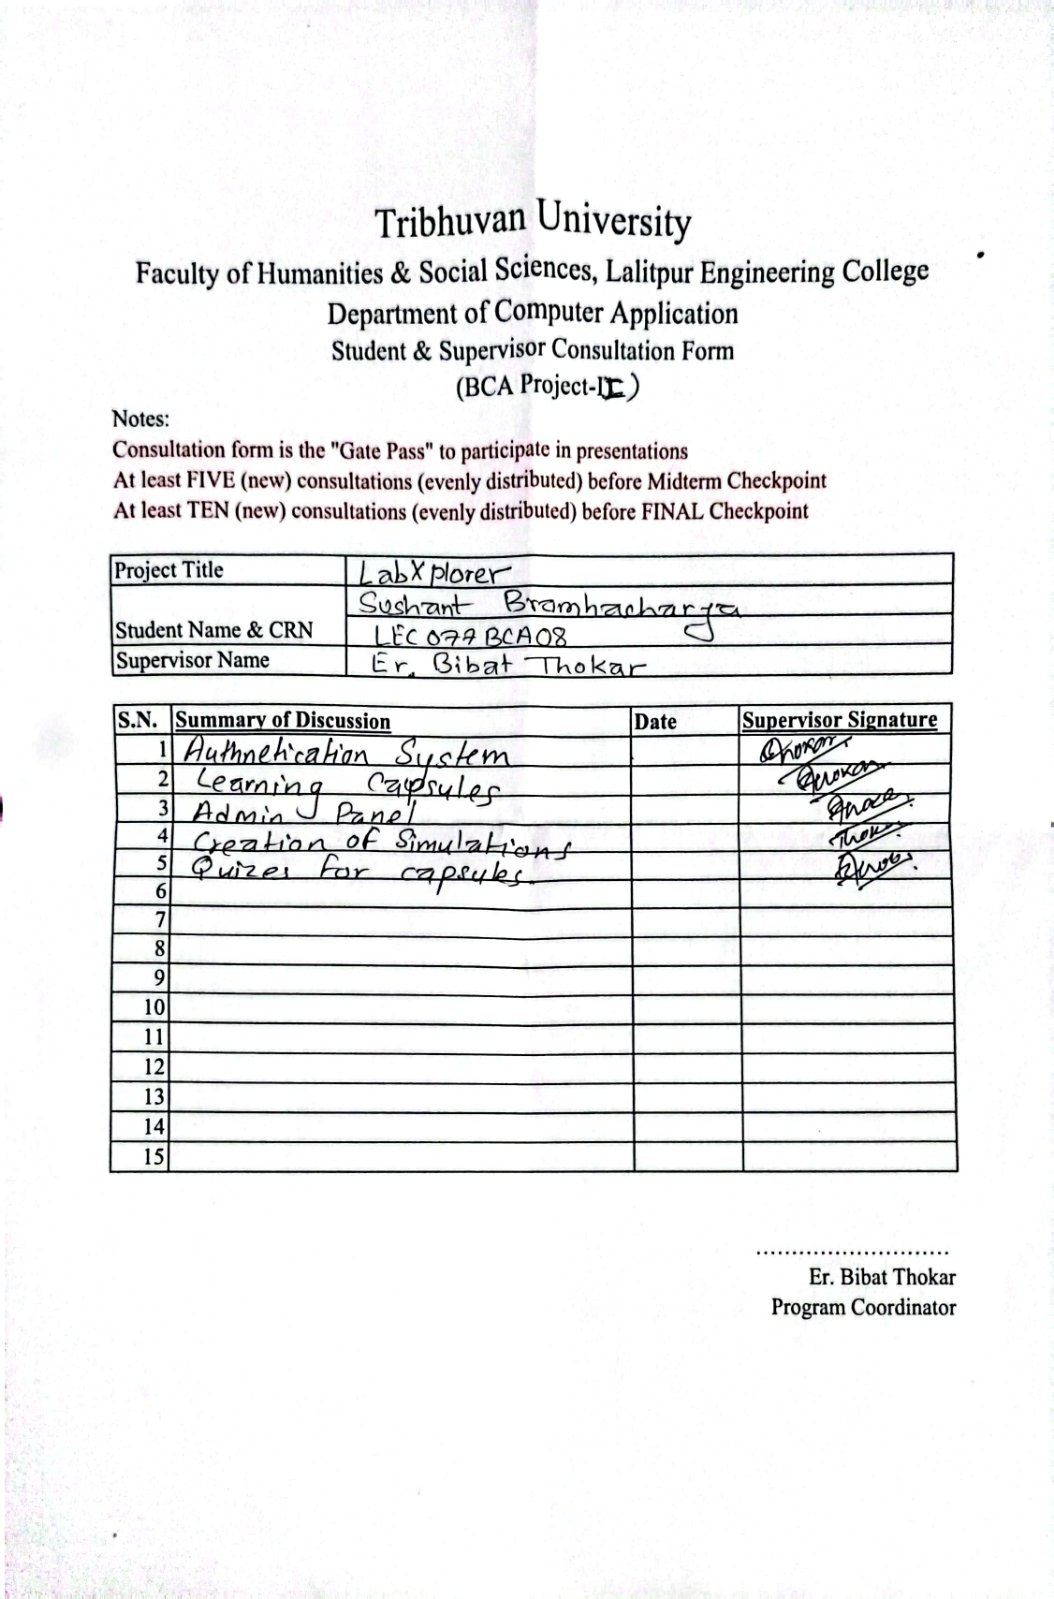
\includegraphics[width=430px]{Diagrams/supervisor.jpg}
    \caption{Supervisor Consultation Form}
\end{figure}
\input{Appendix/appendix2.tex}
\end{appendices}



%========================References setup=========================================================
\newpage
\bibliographystyle{unsrt}
\bibliography{References/references}

\addcontentsline{toc}{chapter}{REFERENCES}

%=============================================================================================



%=========================================================================
\end{document}